\documentclass[10pt,a4paper]{article}
\usepackage[utf8]{inputenc}
\usepackage[T1]{fontenc}
\usepackage[italian]{babel}
\usepackage{amsmath}
\usepackage[a4paper,top=2cm,bottom=3cm,left=3.2cm,right=3.2cm,bindingoffset=0mm]{geometry}
\usepackage{pgfplots}
\pgfplotsset{compat=1.15}
\usepackage{mathrsfs}
\usepackage{amsfonts}
\usepackage{amssymb}
\usepackage{makeidx}
\usepackage{graphicx}

\makeatletter

\newcommand{\newparallel}{\mathrel{\mathpalette\new@parallel\relax}}
\newcommand{\new@parallel}[2]{%
	\begingroup
	\sbox\z@{$#1T$}
	\resizebox{!}{\ht\z@}{\raisebox{\depth}{$\m@th#1/\mkern-5mu/$}}%
	\endgroup
}
\makeatother
\begin{document}
\begin{titlepage}
	\begin{center}
	\vspace*{1cm}
	
	\Huge{\textbf{Spurio's lectures on physics}}
	
	\vspace{0.5cm}
	\Huge{\textbf{Meccanica}}
	
	\vspace{1.5cm}
	
	\Large{Fabio Prestipino}
	
	\vspace{3.5cm}
	\LARGE{Un semplice riassunto per\\
	\textit{"sentire la musica"}$_{ cit. F.S.}$}\\
	
	\vfill

	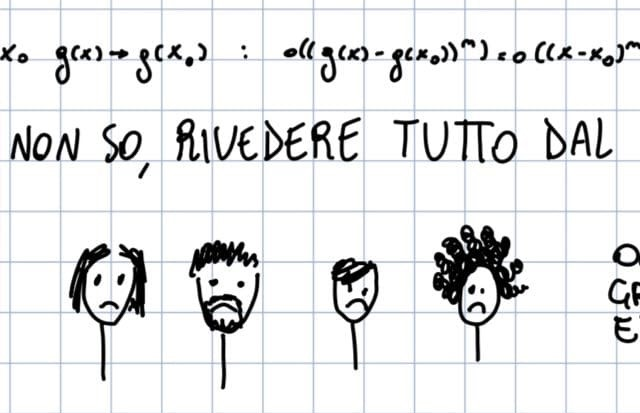
\includegraphics[width=0.6\textwidth]{noi}\\
	\vspace{2cm}
	\Large
	Fisica\\
	Università di Bologna\\
	Dicembre 2021
	
	\end{center}
\end{titlepage}
\newpage
\tableofcontents
\newpage
\section{Cinematica}
\subsection{Introduzione}
La cinematica studia il moto dei corpi approssimati a punti geometrici, ciò è possibile quando le dimensioni del corpo sono trascurabili rispetto alle distanze percorse e non influenzano le caratteristiche del moto. Questa disciplina si avvale dell'uso del potente strumento dell'analisi matematica, in particolare della derivazione ed integrazione rispetto al tempo. La possibilità di usare queste operazioni matematiche si regge sull'ipotesi della continuità del moto, non dimostrabile ma in accordo con i dati sperimentali, che permette di operare con i limiti e dunque di introdurre l'analisi.
\subsection{L'equazione del moto}
La \textbf{traiettoria} è l'insieme di punti occupati dal corpo puntiforme nel suo moto, tale curva può essere descritta da un'equazione vettoriale, dipendente dal tempo: l'equazione del moto.
\begin{equation*}
	\vec{r} = \vec{r}(t)
\end{equation*}
Un punto materiale ha la possibilità di muoversi in tre direzioni: quelle degli assi del piano cartesiano tridimensionale. La funzione vettoriale $\vec{r}$ può essere espressa mediante le sue componenti vettoriali (rappresentazione vettoriale)
\begin{equation*}
\vec{r} = x(t) \hat{i} + y(t) \hat{j} + z(t) \hat{k}
\end{equation*}
O con le sue funzioni scalari
\begin{equation*}
	\begin{cases}
		x = x(t)\\
		y = y(t)\\
		z = z(t)
	\end{cases}\
\end{equation*}
Questa è detta rappresentazione cartesiana della traiettoria.\\
\'{E} possibile infine esprimere $\vec{r}$ in modo da non menzionare caratteristiche geometriche, relative al sistema cartesiano ed enfatizzare le sue caratteristiche cinematiche (rappresentazione intrinseca). Supponiamo di avere la curva di una traiettoria generica, rettificando tale curva, stabilendo un centro O e uno spostamento unitario s, potremo associare ad ogni punto della traiettoria un numero reale s, detto ascissa curvilinea (che rappresenta la lunghezza dell'arco che va dall'origine al punto). Ora esprimiamo il moto in funzione di s ed s in funzione di t
\begin{align*}
	&\vec{r} = \vec{r}(s)\\
	&s = s(t)
\end{align*}
s è detta legge oraria, ed è uno scalare che rappresenta lo spazio percorso. 
\subsection{Velocità}
Consideriamo due istanti $t$ e $t'= t + \Delta t$
\begin{align*}
&\Delta \vec{r} = \vec{r}(t')- \vec{r}(t)
\end{align*}
Questa espressione ci offre solamente la variazione della posizione del punto materiale, senza fornire informazioni sul modo in cui tale spazio viene percorso. Definiamo il vettore velocità media 
\begin{align*}
&\vec{v_m} \equiv \frac{\vec{r}(t+\Delta t) - \vec{r}}{\Delta t}
\end{align*} 
Per una descrizione del vettore velocità in un singolo punto, vorremmo che $\Delta t \rightarrow 0$. Definiamo la velocità istantanea (o più semplicemente, velocità)
\begin{align*}
	&\vec{v} \equiv \lim_{x \to 0} \frac{\vec{r}(t+\Delta t) - \vec{r}}{\Delta t} = \lim_{\Delta t \to 0} \frac{\Delta \vec{r}}{\Delta t} =  \frac{d\vec{r}(t)}{dt}
\end{align*}
Per le proprietà delle derivate, la direzione di $\vec{v}$ è tangente a quella alla traiettoria del punto materiale.\\
Anche per la velocità sono possibili 3 rappresentazioni: quella vettoriale:
\begin{align*}
	&\vec{v} =v_x \hat{i} + v_y \hat{j} + v_z \hat{k}\\
	&= \frac{dx}{dt}\hat{i} +\frac{dy}{dt}\hat{j} + \frac{dz}{dt}\hat{k}\\
	&=\dot{x} \hat{i} + \dot{y} \hat{j} + \dot{z} \hat{k}
\end{align*}
L'ultima riga utilizza la notazione per le derivate sul tempo, introdotta da Newton. 
Quella cartesiana: 
\begin{equation*}
	\begin{cases}
		v_x = \dot{x}(t)\\
		v_y = \dot{y}(t)\\
		v_z = \dot{z}(t)
	\end{cases}\
\end{equation*}
Per la rappresentazione intrinseca introduciamo il versore tangente. Siano P e P' due punti della curva, individuati dalle ascisse curvilinee s e $s' = s + \Delta s$ e $\Delta \vec{r} = \vec{PP'}$. Il modulo del vettore $\Delta \vec{r}$ è uguale al segmento secante che congiunge P e P' mentre $\Delta s$ è uguale all'arco compreso fra P e P' (maggiore di $\Delta r$). Se $\Delta s \rightarrow 0$ allora $\Delta r = \Delta s$. Definiamo dunque il versore tangente
\begin{align*}
	\hat{u_t} \equiv \lim_{\Delta s \to 0} \frac{\Delta \vec{r}}{\Delta s} = \frac{d\vec{r}}{ds}
\end{align*}
Questo versore ha chiaramente modulo 1 e, per le proprietà delle derivate, direzione tangente a $\vec{r}$. Riscriviamo ora il vettore velocità
\begin{align*}
	\vec{v} = \frac{d\vec{r}}{dt} = \frac{d\vec{r}}{ds} \frac{ds}{dt} = \frac{ds}{dt} \hat{u_t}
\end{align*}
Il penultimo passaggio è da interpretare matematicamente come moltiplicazione e divisione per una stessa quantità infinitesima. Il risultato è intuitivamente giustificato: il verso è tangente ad $\vec{r}$ per definizione ed il modulo è uguale all'arco infinitesimo di traiettoria percorso in un tempo infinitesimo. Detto $v_{s}$ il modulo di $\vec{v}$, possiamo finalmente scrivere la rappresentazione intrinseca: 
\begin{align*}
\vec{v} = v_s \hat{u_t} = \dot{s} \hat{u_t}
\end{align*}
\subsection{Accelerazione}
Per l'accelerazione, con considerazioni analoghe a quelle fatte per la velocità, possiamo scrivere
\begin{align*}
	&\vec{a}(t) \equiv \frac{d\vec{v}(t)}{dt} = \frac{d^{2}\vec{r}(t)}{dt^{2}}\\
	&=\ddot{x} \hat{i} + \ddot{y} \hat{j} + \ddot{z} \hat{k}
\end{align*}
\begin{equation*}
	\begin{cases}
		a_x = \ddot{x}(t)\\
		a_y = \ddot{y}(t)\\
		a_z = \ddot{z}(t)
	\end{cases}\
\end{equation*}
L'espressione intrinseca dell'accelerazione è particolarmente importante perché mette in evidenza la presenza di due componenti di direzione diversa, una parallela e una perpendicolare alla velocità. Ricaviamo l'accelerazione dalla derivata della forma intrinseca della velocità
\begin{align*}
\vec{a} = \frac{d\vec{v}}{dt} = \frac{d}{dt}(v_s \hat{u_t}) = \frac{dv_s}{dt} \hat{u_t} + v_s \frac{d\hat{u_t}}{dt}
\end{align*}
Nell'ultimo passaggio è stata semplicemente svolta la derivata di un prodotto. Ricordando $v_s = \frac{ds}{dt}$ possiamo riscrivere il primo componente
\begin{align*}
 \vec{a} = \frac{d^{2}s}{dt^{2}} \hat{u_t} + v_s \frac{d\hat{u_t}}{dt} = \ddot{s} \hat{u_t} + v_s \frac{d\hat{u_t}}{dt}
\end{align*}
Risulta chiaro che il primo componente, ha direzione tangente a quella del moto, per questo viene detta accelerazione tangenziale. Concentriamoci ora sul secondo componente
\begin{align*}
v_s \frac{d\hat{u_t}}{dt} = v_s \frac{d\hat{u_t}}{ds}\frac{ds}{dt} = v_{s}^{2} \frac{d\hat{u_t}}{ds}
\end{align*}
La traiettoria è una curva generica, una curvatura è approssimabile con l'arco di una circonferenza, di raggio $\rho$ e curvatura $\frac{1}{\rho}$.
La derivata $\frac{d\hat{u_t}}{ds}$ rappresenta la variazione di direzione e modulo del vettore tangente in un arco di circonferenza ds. Tale variazione però, visto che il modulo rimane invariato, sarà solo di un angolo $d\varphi$ in un'arco ds, mentre la direzione, per le proprietà delle derivate, sarà perpendicolare a $\hat{u_t}$ e la chiameremo $\hat{u}_n$. 
\begin{equation*}
\frac{d\hat{u_t}}{ds} = \frac{d\varphi}{ds} \hat{u}_n
\end{equation*}
Per comprendere meglio si pensi alla definizione di radiante come angolo al centro corrispondente ad un arco di lunghezza pari al raggio della circonferenza stessa, quindi al rapporto tra l'arco e il raggio corrispondente. Si ha che
\begin{align*}
&d\varphi = \frac{ds}{\rho}\\
\end{align*}
Dunque, mettendo insieme quanto ricavato
\begin{align*}
& v_{s}^{2} \frac{d\hat{u_t}}{ds} = v_{s}^{2} \frac{d\varphi}{ds} \hat{u}_n = \frac{v_{s}^{2}}{\rho} \hat{u}_n\\
\end{align*}
Questa componente, detta accelerazione normale, è perpendicolare alla velocità e punta sempre verso il centro di curvatura, per questo è anche detta accelerazione centripeta. Essa è presente in ogni moto su traiettoria non rettilinea, dunque possiamo dire che ogni moto curvo è accelerato.\\
Riassumendo
\begin{equation*}
\vec{a} = \ddot{s} \hat{u_t} + \frac{\dot{s}^{2}}{\rho} \hat{u}_n
\end{equation*}
\section{Applicazioni della cinematica}
\subsection{Moto rettilineo uniforme}
 Questo tipo di moto ha come traiettoria una retta, dunque è possibile studiarlo solamente su un'asse, ad esempio quello delle x. Non essendoci accelerazioni, determinare la legge oraria risulta particolarmente semplice, ricordiamo che
\begin{align*} 
& \frac{dx}{dt}= \dot{x}\\
& dx = \dot{x} dt\\
& \int dx = \int \dot{x}(t) dt
\end{align*}
Ma, sapendo che la velocità è costante ($\dot{x}(t) = \dot{x}_0$), 
\begin{align*} 
& x(t) = \dot{x}_0\int dt = \dot{x}_0 t + C
\end{align*}
Dove C è la posizione $x_0$ all'istante t = 0.
\begin{align*} 
& x(t)=  \dot{x}_0 t + x_0
\end{align*}
Da un punto di vista vettoriale
\begin{equation*}
\vec{r} = (\dot{x}_0 t + x_0)\hat{i} + 0 \hat{j} + 0 \hat{k}
\end{equation*}
Mentre da uno cartesiano
\begin{equation*}
	\begin{cases}
		r_x = \dot{x}_0 t + x_0\\
		r_y = 0\\
		r_z = 0
	\end{cases}\
\end{equation*}
\subsection{Moto rettilineo uniformemente accelerato}
In questo caso abbiamo $\frac{d\dot{x}}{dt}=\ddot{x}_0$. Integriamo due volte questa espressione per ottenere x
\begin{align*}
&\dot{x} = \int \ddot{x}_0 dt = \ddot{x}_0 \int dt = \ddot{x}_0 t + C && C= \dot{x}_0\\
&x = \int \dot{x} dt = \int (\ddot{x}_0 t + \dot{x}_0) dt= \int \ddot{x}_0 t dt + \int \dot{x}_0 dt = \frac{1}{2} \ddot{x}_0 t^2 + \dot{x}_0 t + C && C = x_0
\end{align*}
Da un punto di vista vettoriale
\begin{equation*}
	\vec{r} = (\frac{1}{2} \ddot{x}_0 t^2 + \dot{x}_0 t + x_0)\hat{i} + 0 \hat{j} + 0 \hat{k}
\end{equation*}
Mentre da uno cartesiano
\begin{equation*}
	\begin{cases}
		r_x = \frac{1}{2} \ddot{x}_0 t^2 + \dot{x}_0\ t + x_0\\
		r_y = 0\\
		r_z = 0
	\end{cases}\
\end{equation*}
\subsection{Moto parabolico}
Questo tipo di moto è particolarmente importante perché sulla terra è sempre presente un'accelerazione costante: quella di gravità. Un corpo in caduta libera avrà un'accelerazione $\ddot{z} = g = 9.8 m/s^2$. Essendo diretta verso il centro della terra, questa accelerazione sarà negativa e sull'asse z; l'equazione del moto diventerà dunque
\begin{equation*}
	\vec{r} = 0\hat{i} + 0 \hat{j} + (-\frac{1}{2} g t^2 + \dot{x}_0 t + z_0) \hat{k}
\end{equation*}
Se però il corpo non cade sulla verticale ma è lanciato con una certa velocità $v_0$ (ad esempio la traiettoria di un proiettile sparato da un cannone inclinato rispetto al suolo di un angolo $\theta$), il moto sarà una composizione di quello rettilineo uniforme nell'asse x ed uniformemente accelerato nell'asse z
\begin{equation*}
	\vec{r} = (\dot{x}_0 t + s_0)\hat{i} + 0 \hat{j} + (\dot{x}_0 t + x_0) \hat{k}
\end{equation*}
La traiettoria del corpo sarà dunque una parabola e il caso della caduta libera sulla verticale può essere vista come un caso particolare di quest'ultimo con $\dot{x}_0 = 0$.
\subsection{Moto circolare uniforme}
Cominciamo con il definire alcune grandezze utili per lo studio del moto circolare.
\begin{itemize}
\item $\vec{r}(t)$ = vettore raggio, con estremi il centro della circonferenza e il punto materiale
\item r = lunghezza del raggio della circonferenza
\item T = tempo impiegato per compiere un giro della circonferenza ("periodo")
\item $\vec{\omega}_0$ = $\frac{2\pi}{T}$   ("velocità angolare o di spazzata")
\item $\theta(t)$ = $\omega_0\ t$ (angolo a cui si trova il punto materiale)
\item $\vec{v}_0$=$\frac{2\pi}{t} \vec{r}$ ("velocità tangenziale")
\end{itemize}
Come visto nella sezione precedente, qualunque moto non rettilineo ha sempre un'accelerazione centripeta, ne segue che l'espressione "uniforme" si riferisce alla velocità angolare $\vec{\omega}$ (spazza archi uguali in tempi uguali). Studiamo ora equazione del moto, velocità e accelerazione, il moto circolare avviene sul piano quindi le coordinate di interesse saranno solamente x,y
\begin{align*}
\vec{r}(t)=
\begin{cases}
x(t)= r\ \cos (\theta) = r\ \cos (\omega t)\\
y(t)= r\ \sin (\theta) = r\ \sin (\omega t)
\end{cases} 
\end{align*}
Come sempre, la velocità si ottiene derivando l'equazione del moto
\begin{align*}
	\vec{v}_0(t)=
	\begin{cases}
		\dot{x}(t)= -r\ \omega\ \sin (\omega t)\\
		\dot{y}(t)= r\ \omega\ \cos (\omega t)
	\end{cases} 
\end{align*}
Già sappiamo, per le proprietà delle derivate, che il vettore velocità avrà direzione perpendicolare a quella del moto, per verifica possiamo svolgere il prodotto scalare (che è uguale a zero per vettori perpendicolari)
\begin{align*}
	&\vec{r} \cdot \vec{v_0} = x \dot{x} + y \dot{y} = (r\ \cos \omega t) (-r\ \omega\ \sin \omega t) + (r\ \sin \omega t) (r\ \omega\ \cos \omega t)\\
	&= -r^2\ \omega\ (\cos (\omega t)\ \sin( \omega t)) + r^2\ \omega\ (\cos (\omega t)\ \sin( \omega t)) = 0 &&c.v.d.
\end{align*}
L'equazione vettoriale della velocità  sarà
\begin{equation*}
\vec{v} = r\ \omega \hat{\tau}
\end{equation*}
Dove $\hat{\tau}$ è il vettore tangente alla traiettoria.\\
Lo scopo che or ci proponiamo è quello di scrivere in forma intrinseca la velocità. Cominciamo con l'introdurre il versore perpendicolare sia alla traiettoria sia alla velocità sfruttando la proprietà del prodotto vettoriale, che da come risultato un vettore perpendicolare ad entrambi i vettori del prodotto.
\begin{equation*}
	\hat{k} \equiv \hat{r} \times \hat{\tau}
\end{equation*}
Possiamo così riscrivere la velocità angolare $\vec{\omega}$
\begin{equation*}
	\vec{\omega} = \omega \hat{k}
\end{equation*}
\'{E} necessario fare una precisazione: esistono due tipi di vettori, quelli polari, in cui la direzione del vettore coincide con quella del moto (come tutti quelli visti fin ora: $\vec{r}, \vec{v}, \vec{a}$) e quelli assiali, in cui il vettore, convenzionalmente, indica la normale al piano su cui avviene il movimento. L'espressione appena usata per $\vec{\omega}$ è di tipo assiale, infatti la velocità angolare agisce sul piano della circonferenza mentre $\vec{k}$ è ad esso perpendicolare.\\
Scriviamo ora la velocità tangenziale in forma intrinseca
 \begin{equation*}
 	\vec{v} = \vec{\omega} \times \vec{r}
 \end{equation*}
A partire da questa forma è possibile ricavare la forma vettoriale esplicitando i due vettori del prodotto in forma modulo-versore
 \begin{equation*}
	\vec{v} = \vec{\omega} \times \vec{r} = \omega \hat{k} \times r \hat{r} = \omega r \hat{k} \times \hat{r} = \omega r \hat{\tau}
\end{equation*}
Mentre svolgendo il prodotto vettoriale si giunge alla forma cartesiana. \\
L'accelerazione, ottenibile derivando la velocità, risulta 
\begin{align*}
&\vec{a}=
	\begin{cases}
		a_x = -r \omega^2\ \cos(\omega t)\\
		a_y = -r \omega^2\ \sin(\omega t)
	\end{cases}\\
&a = \sqrt{a_x^2 + a_y^2}= r\ \omega^2
\end{align*}
Il modulo dell'accelerazione è costante essendo la velocità angolare (e dunque anche tangenziale) costanti in modulo. In questo caso l'accelerazione tangenziale è nulla La derivata della velocità tuttavia non è nulla perché il suo verso non è costante. Ricordando l'introduzione generale del concetto di accelerazione nella sezione precedente, la componente tangente è nulla mentre quella centripeta è costante in modulo. Definendo il versore $\hat{r}$ come vettore posizione fratto il suo modulo ($\vec{r}$/r) è possibile scrivere l'accelerazione in forma vettoriale
\begin{align*}
	&\hat{r} \equiv \frac{r(\cos\omega t \cdot \hat{i} + \sin \omega t \cdot \hat{j})}{r} = (\cos\omega t \cdot \hat{i} + \sin \omega t \cdot \hat{j})\\
	&\vec{a} = -\omega^2 r \hat{r} = -\omega^2 r\ (\cos\omega t \cdot \hat{i} + \sin \omega t \cdot \hat{j})
\end{align*}
Per ottenere la forma intrinseca è sufficiente derivare la forma intrinseca della velocità
\begin{equation*}
	\frac{d\vec{v}}{dt} = \frac{d\vec{\omega}}{dt} \times \vec{r} + \vec{\omega} \times \frac{d\vec{r}}{dt} = \vec{\omega} \times \vec{v} = \vec{\omega} \times (\vec{\omega} \times \vec{r})
\end{equation*}
Dove nel secondo passaggio si è svolta la derivata di prodotto da cui poi è stato eliminato il primo addendo poiché la derivata dalla velocità angolare risulta nulla in quanto costante per ipotesi. Il risultato finale è la forma ricercata, è possibile svilupparla utilizzando la regola del BAC-CAB (doppio prodotto vettoriale) per ottenere la forma vettoriale. 
\subsection{Moto circolare non uniforme}
In questo caso, generalizzazione di quello precedente, abbiamo che $\vec{\omega}$ non è costante ma dipende dal tempo ($\vec{\omega}(t)$). Ciò comporta che ora la velocità tangenziale avrà sia modulo che verso dipendenti dal tempo. L'unica differenza di interesse sta nell'accelerazione
\begin{align*}
	\vec{a} &=\frac{d\vec{v}}{dt}= \frac{d}{dt} (\vec{\omega} \times \vec{r}) = \frac{d\vec{\omega}}{dt} \times \vec{r} + \vec{\omega} \times \frac{d\vec{r}}{dt} =\\
	 &=\hat{k}\ \frac{d\omega}{dt} \times r \cdot \hat{r} + \vec{\omega} \times (\vec{\omega} \times \vec{r}) =\\ &=\dot{\omega} r\ \hat{\tau} - \omega^2 r \hat{r}
\end{align*}
Oltre all'accelerazione centripeta, che permette al moto di essere circolare, è presente anche un altro termine, l'accelerazione tangenziale, che indica il variare della velocità tangenziale rispetto al tempo.
\section{Le leggi della dinamica}
Se la cinematica studia il movimento di punti materiali, la dinamica si propone di studiare le cause di tale movimento. Sperimentalmente nasce la necessità di introdurre una grandezza che porti un corpo a muoversi: la forza. 
\subsection{Primo Principio}
 Aristotele sosteneva che per muovere un corpo è necessario applicarvi una forza per tutta la sua traiettoria, ciò fu smentito da Galileo che intuì che l'errore di Aristotele stava nel non aver considerato le forze d'attrito. In generale, ci si rende conto che in assenza di forze esterne un corpo che ha una certa velocità tende a mantenerla costante (anche se fosse nulla): lo "stato naturale" di un corpo è quello di moto rettilineo uniforme. \'{E} chiaro che questa intuizione è riscontrabile solo in alcuni tipi di sistemi di riferimento, che vengono detti inerziali (S.R.I.) che sono tali se e solo se un corpo in moto mantiene la sua velocità costante in assenza di forze. Nel mondo reale, un comodo sistema di riferimento inerziale è quello con origine nel sole e con assi le rette che puntano alle stelle fisse, questo perché nonostante tutti i corpi interagiscano sempre fra loro, a debita distanza tali interazioni sono trascurabili (i corpi celesti più vicini sono abbastanza lontani dal sistema solare). Nei S.R.I. sono valide le intuitive leggi di relatività galileiana. Possiamo enunciare il Primo Principio della dinamica:\\
 \textit{Un corpo in un S.R.I. non soggetto a forze permane nel suo stato di quiete o di moto rettilineo uniforme.}
 \subsection{Secondo Principio}
 La forza ha l'effetto di far variare la velocità di un corpo (e quindi metterlo in moto), dunque deve essere sicuramente proporzionale all'accelerazione. Sperimentalmente si nota che questa proporzionalità è diretta a meno di una costante: la massa. La massa è una caratteristica dei corpi molto difficile da definire, per i nostri scopi possiamo dire che è una grandezza che ha l'effetto di opporsi ad una modifica di velocità del corpo stesso (massa inerziale), questo concetto è attribuibile anche al punto materiale, in cui tutta la massa è concentrata nel singolo punto. Ancora, ci si rende conto che le stesse forze che mettono in moto i corpi possono anche deformarli, da questa semplice intuizione nasce il dinamometro, uno strumento di misura della forza che sfrutta le proprietà delle molle che vedremo nella prossima sezione. Sperimentalmente, avvalendosi del dinamometro, si ottiene che per sommare più forze è necessario ricorrere alle regole di somma di vettori, le forze sono grandezze vettoriali. Enunciamo il Secondo Principio della dinamica:\\
 \textit{In un S.R.I. l'accelerazione di un corpo è sempre dovuta all'azione di forze; tra forza risultante e accelerazione sussiste la relazione $\sum_{i} \vec{f}_i = m \cdot \vec{a}$.}
\section{Applicazioni delle leggi della dinamica}
Le forze agenti sui corpi contengono tutte le informazioni per conoscere il loro moto, lo studio delle forze diventa così lo scopo principe della fisica. Vediamo alcuni esempi di questo approccio.
\subsection{Il pendolo semplice e la forza peso} \label{sec:pendulum}
Cominciamo col definire alcune grandezze utili:
\begin{itemize}
\item S = arco di circonferenza che percorre il pendolo
\item l = lunghezza del pendolo
\item $\theta(t) = \frac{S}{l} = \omega \cdot t$
\item T = tempo impiegato per un'oscillazione completa, due archi ("periodo")
\item $\vec{\omega}$ = $\frac{2 \pi}{T}$ ("velocità angolare")
\item $\vec{F}$ = forza peso
\item $\vec{T}$ = forza di tensione del filo, per definizione uguale e contraria alla forza che vi è applicata.
\end{itemize}
Scegliamo l'origine degli assi di riferimento nella massa all'estremità del pendolo quando si trova in posizione + $\theta$ (ampiezza massima positiva), l'asse x sarà sempre perpendicolare al filo, che sarà il nostro asse y. Per convenzione, assumiamo l'alto come verso positivo per l'asse y e la destra per l'asse x. Le forze essendo vettori si sommano con la regola del parallelogramma. La tensione è positiva ed in direzione dell'asse y mentre la forza peso (sempre diretta verso il centro della terra) ha una componente negativa ed in direzione dell'asse y (uguale e contraria, per definizione alla forza tensione) ed una componente negativa in direzione dell'asse x. Possiamo calcolare la risultante delle forze sul pendolo
\begin{align*}
	\sum_{i} \vec{F}_i = 
	\begin{cases}
		F_x = -f_x = - mg\ \sin(\theta)\\
		F_y = t_y -f_y = mg\ \cos(\theta) - mg\ \cos(\theta) = 0
	\end{cases}
\end{align*}
Possiamo riscrivere il secondo principio della dinamica in forma differenziale vedendo l'accelerazione come derivata seconda dell'arco $S$ (spazio percorso) per poi risolvere l'equazione differenziale che ne risulta eguagliando la forza risultante appena ottenuta
\begin{align}\label{eq:pendulum}
&m \frac{d^2 S}{dt^2} = -mg\ \sin \theta
\end{align}
\begin{align*}
	&\frac{d^2 \theta \cdot l}{dt^2} = -g\ \sin \theta\\
	&\frac{d^2 \theta}{dt^2} = -\frac{g}{l}\ \sin \theta
\end{align*}
L'analisi matematica ci dice che non esiste soluzione analitica a questa espressione ma è possibile operare un'ottima approssimazione con la serie di Taylor (è sufficiente la prima approssimazione per piccole oscillazioni)
\begin{align*}
&\sin\theta = \sum_{n=0}^{\infty} \frac{(-1)^n}{(2n)!} x^{2n} = \theta- \frac{\theta^3}{6}+\frac{\theta^5}{120}- \frac{\theta^7}{5040}-...\\
&\frac{d^2 \theta}{dt^2} \simeq -\frac{g}{l}\ \theta
\end{align*}
Matematicamente, la soluzione di questa equazione differenziale può essere equivalentemente una delle seguenti
\begin{align*}
	\theta(t)=
	\begin{cases}
		k\cdot \sin(\omega t)\\
		k \cdot \cos(\omega t)
	\end{cases}
\end{align*}
Prima di sapere quale delle due sia la soluzione corretta, riflettiamo sulla costante moltiplicativa k che compare dalla risoluzione dell'equazione: essa rappresenta l'angolo massimo $\theta_0$ raggiungibile dal pendolo, è una grandezza adimensionale. Da ciò ne deriva che, quando $t= 0$, per come è stato impostato il nostro sistema, $\theta (t) = \theta_0$ e quindi 
\begin{align*}
	\theta(0)=
	\begin{cases}
    \theta_0 \cdot \sin(0) = 0\\
    \theta_0 \cdot \cos(0) = \theta_0
	\end{cases}
\end{align*}
Risulta chiaro che la soluzione con il seno non è accettabile. Tuttavia la differenza che intercorre fra le due soluzioni è solamente di 1/4 T, infatti se l'origine del sistema fosse stata a $\theta = 0$ la soluzione accettabile sarebbe stata quella con il seno. \\
Non ci resta che determinare la costante $\omega$, che potremmo vedere come la velocità angolare media che ha il pendolo in una sua oscillazione. Per farlo eguagliamo l'equazione differenziale ottenuta dal calcolo delle forze con quella ottenuta derivando due volte il risultato appena ottenuto
\begin{align*}
&\frac{d^2}{dt^2} (\theta_0 \cdot \cos(\omega t)) = -\frac{g}{l} \theta\\
&\frac{d}{dt} (-\theta_0\ \omega \cdot \sin(\omega t)) = -\frac{g}{l} \theta\\
&-\theta_0\ \omega^2 \cdot \cos(\omega t) = -\frac{g}{l} \theta\\
\end{align*}
Sappiamo, dalla risoluzione dell'equazione differenziale che $\theta = \theta_0 \cos(\omega t)$
\begin{align*}
	&\omega = \sqrt{\frac{g}{l}}\\
	&\theta(t) = \theta_0\ \cos(\sqrt{\frac{g}{l}}\ t)
\end{align*}
Questa è la legge oraria del pendolo semplice. Si noti che non dipende dalla massa del pendolo e che il grafico è sinusoidale.\\ Fra le varie applicazioni interessanti vale la pena evidenziarne due: l'orologio a pendolo e il calcolo della costante di gravità g.\\
Ricordando la definizione di $\omega$ come $\frac{2 \pi}{T}$ ed eguagliando con la nuova equazione di $\omega$ otteniamo
\begin{align*}
T = 2\pi \sqrt{\frac{l}{g}}
\end{align*}
Si noti che le grandezze del secondo membro dell'equazione sono tutte costanti, si è trovato un modo per ottenere un oggetto che possa segnare il tempo con periodo costante. \'{E} possibile tarare il pendolo modificandone la lunghezza in modo da avere T = 1s e, mantenendo il pendolo sotto determinate condizioni (principalmente in assenza di attrito) è possibile ottenere un'orologio.\\
Inoltre, isolando g nell'equazione precedente, si nota che questa grandezza è facilmente calcolabile con misure di tempo, questo perché a seconda della gravità presente nel luogo il periodo di oscillazione varia. Questo metodo veniva usato da Newton e contemporanei nel XVII secolo.
\subsection{Le molle e la forza elastica}
Si verifica sperimentalmente che una forza applicata ad una molla in quiete ne provoca l'estensione in modo direttamente proporzionale ad essa fin quando non si torna ad una situazione stabile: la forza applicata alla molla è stata bilanciata da una forza uguale e di verso contrario esercitata dalla molla. La forza che imprime la molla deve dunque essere proporzionale all'estensione e di segno negativo perché opposta alla forza applicata. 
\begin{align*}
	\vec{F}_e = -k \cdot x
\end{align*}
Dove k è una costante che dipende dalle caratteristiche della molla (materiale, dimensione e densità delle spire...) e, per l'analisi dimensionale, ha dimensioni $[M][T]^{-2}$.
Eguagliando questa equazione alla forma differenziale del Secondo Principio della dinamica, considerando l'accelerazione come la derivata seconda dello spazio percorso dalla molla nella sua estensione otteniamo
\begin{align*}
	&m \frac{d^2x}{dx^2} = -kx\\
	&\frac{d^2x}{dx^2} = -\frac{k}{m}x\\
\end{align*}
Questa equazione differenziale è dello stesso tipo di quella vista nel paragrafo precedente, la soluzione è
\begin{align*}
	x(t) = x_0 \cdot \cos(\omega t)
\end{align*}
Dove x è la posizione della molla e $x_0$ è la posizione di massima estensione(quando si tira la molla), lo 0 è la posizione iniziale di quiete. Una molla sollecitata oscilla nell'intervallo $+x_0$ e $-x_0$.\\
Per determinare $\omega$, procediamo analogamente a come fatto per il pendolo, derivando l'equazione ottenuta due volte ed eguagliandola all'equazione differenziale ottenuta dal Secondo Principio.
\begin{align*}
	&\frac{d^2x}{dt^2}= -x_0 \omega^2 \cos(\omega t) = -\frac{k}{m}x\\
	&\omega = \sqrt{\frac{k}{m}}
\end{align*}
Lo studio della forza elastica, al di là dello studio delle molle, è di estremo interesse perché vari sistemi di corpi si comportano in modo descrivibile in prima approssimazione con le leggi appena trovate.
\subsubsection*{Molle non vincolate ad una parete}
\'{E} fondamentale notare che fin ora abbiamo trattato molle vincolate per un estremo alla parete, se ciò non dovesse accadere le forze che esercita la molla hanno modulo e direzione uguale ma verso sia positivo che negativo! Un esempio intuitivo lo abbiamo quando comprimiamo una olla fra le nostre mani e poi lasciamo cadere la molla staccando contemporaneamente entrambe le mani da essa, nonostante fosse inizialmente compressa essa cadrà verticalmente perché le forze che esercita si annullano. Se invece avessimo tolto solamente una mano la molla si sarebbe spostata con accelerazione orizzontale $-k \Delta x$. Vediamo ora un'esempio più rigoroso: si consideri un filo inestensibile vincolato alla parete per un estremità e con attaccata la massa $m_1$ sull'altra estremità, a cui a sua volta è attaccata una molla a cui è attaccata un'altra massa $m_2$, il sistema è in equilibrio. Una forza esterna comprime la molla alzando quindi anche la massa $m_2$, qual'è la tensione sul filo? Essendo il sistema in quiete sappiamo che la somma delle forze è nulla quindi
\begin{align*}
	&T + F_{p1}+F_{p2}+F_{ext}+F_e = 0\\
	&T -m_1g-m_2g+(m_2g + k\Delta x) + (-k\Delta x + k\Delta x)= 0\\
	\Rightarrow & T = m_1 g - k \Delta x 
\end{align*}
la forza esterna si limita a bilanciare il peso della massa e a caricare la molla, essa esercita una forza verso il basso che compensa quella della forza esterna e una verso l'alto che diminuisce la tensione. 
\subsection{Forza d'attrito radente}
Cominciamo con l'introdurre il concetto di reazione vincolare: ogni corpo che esercita una forza su un piano, ne riceve un'altra uguale e contraria dovuta alle interazioni elettriche fra gli atomi del piano (una bottiglia su un tavolo esercita una forza sul tavolo bilanciata dalla forza che il tavolo esercita sulla bottiglia).\\
Immaginiamo un corpo di massa m in quiete su un piano orizzontale. dall'esperienza risulta ovvio che inclinando progressivamente il piano, si hanno 4 situazioni possibili al variare di $\theta$:\\
\begin{itemize}
\item $0 \leq \theta < \theta^*$: Il corpo è in quiete ;
\item $\theta = \theta^*$: Il corpo rimane in quiete;
\item $\theta > \theta^*$: Il corpo è in moto sul piano inclinato;
\item $\theta > 90$\textdegree: Il corpo è in caduta libera.
\end{itemize}
Analizziamo ognuno di questi punti.\\
Nel primo caso la somma delle forze dovrà sempre essere uguale a zero perché il corpo è in quiete. La forza peso, che si applica sempre verso il centro della terra, può essere scomposta in una componente perpendicolare al piano ($P_\perp$) ed una parallela ($P_\shortparallel$). Sappiamo che la forza di reazione vincolare annulla la forza perpendicolare, ma cosa annulla quella parallela, impedendo il moto del corpo? Questa forza è proprio quella d'attrito statico, generata dalle irregolarità (anche microscopiche) del piano inclinato e del corpo. questa forza viene detta di tipo \textbf{reattivo} cioè dipende da un'altra forza e non può mai superarla (sarebbe assurdo vedere un corpo fermo su di un piano inclinato risalire per la forza d'attrito). Notiamo che il corpo rimane in quiete per tutti gli angoli compresi fra zero e $\theta$, la componente parallela al piano della forza di gravità però aumenta all'aumentare di $\theta$ e quindi per mantenere il corpo fermo anche l'attrito statico dovrà aumentare. L'attrito dunque si "adatta" alla forza che lo genera.  
\begin{align*}
\vec{F}_p= m\vec{g}\ \cos(\theta)=m\vec{g}\\
\vec{R}=-\vec{F}_p=-m\vec{g}\\
\vec{F}_p+\vec{R}= m\vec{g}-m\vec{g}=0
\end{align*}
Nel secondo caso si giunge ad un angolo critico $\theta*$ tale che la forza di attrito statico, è uguale in modulo a $P_\perp$ e con verso opposto. Se $\theta$ aumentasse di una quantità infinitesima, il corpo entrerebbe in moto. Ne deduciamo dunque che esiste una forza massima che può assumere l'attrito statico e che dipende dal coefficiente adimensionale (che dipende dalle caratteristiche del piano) $\mu_s$: $F_a\leq \mu_s R$ dove R è la reazione vincolare del piano.
\begin{align*}
&\vec{F}_p =
\begin{cases}
F_x=P_\shortparallel= mg\ \cos\theta^*\\
F_y=P_\perp=mg\ \sin\theta^*
\end{cases}\\
&\vec{R} = - P_\perp = - mg\ \cos\theta^*\\
&\mu_s=-P_\shortparallel=-mg\ \sin\theta^*
\end{align*}
Determiniamo la costante $\mu_s$ 
\begin{align*}
&\mu_s mg\ \cos \theta^* = mg\ \sin\theta^*\\
&\mu_s=\frac{\sin\theta^*}{\cos\theta^*}=tan\theta^*
\end{align*}
da cui è possibile calcolare sperimentalmente il valore di $\mu_s$.\\
Nel terzo caso, non è più possibile parlare di attrito statico in quanto il corpo è in movimento, introduciamo quindi il coefficiente di attrito dinamico $\mu_d$ che è sempre minore di quello statico (sperimentalmente). Analogamente al caso precedente, $P_\perp = -R$, che si annullano, dunque le uniche forze in gioco sono l'attrito dinamico e $P_\shortparallel$.
\begin{align*}
&\sum_{i} F_i= m \frac{d^2 x}{dt^2}= P_\shortparallel+\mu_d= mg\ \sin\theta-\mu_d\ m g\ \cos\theta\\
&\frac{d^2 x}{dt^2}=g\ \sin\theta-\mu_d g\ \cos\theta\\
&x(t) = \frac{1}{2} gt^2 (\sin\theta-\mu_d\cos\theta)+v_0t
\end{align*}
Quest'ultima è la legge oraria del moto su piano inclinato con attrito dinamico per sfregamento.\\
Nel quarto caso, essendo il piano inclinato di 90\textdegree, la legge oraria diventa
\begin{align*}
x(t) = \frac{1}{2} g t^2 (\sin90-\mu_d \cos90)+v_0t = \frac{1}{2} g t^2 + v_0t
\end{align*}
Che è proprio la legge oraria del moto di caduta libera.
\subsection{Forza d'attrito viscoso}
Immaginiamo un recipiente pieno di un fluido, immergiamo un corpo che cade sulla verticale. Per studiare il moto del corpo possiamo limitarci a considerare solamente l'asse z, dove avviene il moto. Per questa ragione possiamo omettere l'uso dei vettori e concentrarci solamente sui moduli. Sperimentalmente si ottiene che la forza d'attrito è proporzionale alla velocità, a meno di una costante $\eta$, la direzione è la stessa del moto mentre il verso è opposto. Da considerazioni dimensionali risulta chiaro che questa costante ha dimensione $\frac{kg}{s}$.
\begin{align*}
&F_a=-\eta\cdot v\\
&F_p=mg\\
&\sum_{i}F_i=m\frac{dv}{dt}=mg-\eta v
\end{align*}
Questa è l'equazione di un corpo in caduta in un fluido. Cominciamo con il dare un'interpretazione fisica a quanto ottenuto: vogliamo avere un'idea della forma che assumerà il grafico della velocità sul tempo, per far ciò consideriamo due casi limite.\\
Per $t\rightarrow 0$, visto che il corpo viene lasciato senza imprimere alcuna velocità iniziale, il corpo è fermo ed ancora non è passato tempo a sufficienza per cui l'accelerazione possa essere rilevante: $v_{t\rightarrow 0} \simeq 0$.

\begin{align*}
&\frac{dv}{dt}=g
\end{align*}

La derivata della velocità è costante e positiva, ciò significa che la curva "velocità su tempo" cresce linearmente vicino allo 0.\\
Per $t \rightarrow \infty$ , visto che per buonsenso fisico la forza d'attrito non può essere maggiore della forza esercitata dal corpo, dovrà sicuramente esistere un tempo critico $t^*$ tale che $mg=\eta v$, così da avere $m\frac{dv}{dt}=0$ (velocità costante). Ne deduciamo che il grafico "velocità su tempo" dovrà stabilizzarsi su un certo valore finito dopo un tempo $t^*$. Questo tipo di trattazione approssimata ci fornisce una valida idea ma non abbiamo informazioni sulla parte centrale della curva, ricorriamo per questo ad un più approfondito studio matematico.
\begin{align*}
&\vec{F}=m\frac{dv}{dt}=\frac{m}{\eta}\frac{d( \eta v)}{dt}= \frac{m}{\eta}\frac{d (\eta v - mg)}{dt}=mg-\eta v\\
\end{align*}
\'{E} possibile sommare o sottrarre quantità costanti all'interno dell'argomento della derivata perché si annulleranno in ogni caso (come nel caso di $-mg$). Cambiamo variabile $x = \eta v - mg $
\begin{align*}
&\frac{m}{\eta}\frac{dx}{dt}=-x\\
&\frac{dx}{x}=-\frac{\eta}{m} dt\\
&\int_{x(t=0)}^{x(t)}\frac{dx}{x} = \int_{0}^{t_f}-\frac{\eta}{m} dt\\
&[ln(x)]^{x(t)}_{x(t=0)} = [-\frac{\eta}{m} t]^{t =t_f}_{t=0}\\
&ln(x(t))-ln(x(t=0))=-\frac{\eta}{m} t_f\\
&ln(\frac{x(t)}{x(t=0)})=-\frac{\eta}{m} t_f\\
&e^{ln(\frac{x(t)}{x(t=0)})} = e^{-\frac{\eta}{m} t_f}\\
&\frac{x(t)}{x(t=0)} = e^{-\frac{\eta}{m} t_f}
\end{align*}
Cambiamo nuovamente la variabile $x$
\begin{align*}
&\frac{\eta v(t)-mg}{0-mg}=1 - \frac{\eta v(t)}{mg}= e^{-\frac{\eta}{m} t_f}\\
&v(t) = \frac{mg}{\eta}(1-e^{-\frac{\eta}{m}t_f})
\end{align*}
Quest'ultima è l'equazione della velocità di un corpo in caduta in un fluido, è possibile così tracciare l'intero grafico "velocità su tempo", ci si rende conto che le previsioni fatte corrispondono con lo studio di funzione.
\begin{figure}[h]
	\centering
	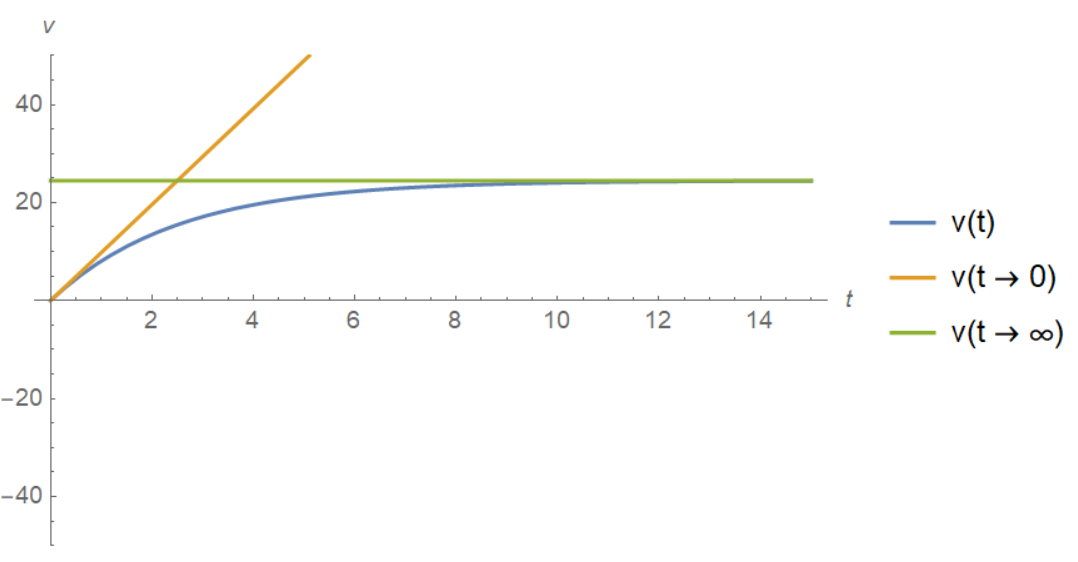
\includegraphics[width=0.7\linewidth]{FluidFriction}
	\caption[Figura 1:]{Grafico "velocità su tempo" con indicate le rette-limite.}
	\label{fig:fluidfriction}
\end{figure}
\subsection{Generalizzazione del metodo}
Come visto, il moto del pendolo semplice e quello della molla presentano molte somiglianze: entrambi sono periodici, e le relative leggi orarie sono ottenibili dalla risoluzione di un'equazioni differenziali del tutto analoghe. Generalizziamo quanto visto dicendo che, se un corpo si muove a causa di forze del tipo
\begin{align}\label{eq:differenziale}
	F= ma = m \ddot{x} = -K x
\end{align}
dove K è una costante, allora la legge oraria sarà del tipo
\begin{align*}
	x(t) = A\sin(\omega t) \quad \text{oppure} \quad x(t) = A\cos(\omega t)
\end{align*}
la scelta fra le due dipende esclusivamente dalle condizioni iniziali in cui si trova il sistema. Ad esempio nel caso del pendolo sceglieremo il coseno se il pendolo parte da fermo ad un angolo $\theta_{max}$ e il seno se parte dall'angolo zero con una certa velocità iniziale. Una volta fatta questa decisione la risoluzione dell'equazione differenziale (\ref{eq:differenziale}) è sempre la medesima e a questo punto consiste semplicemente nel determinare le costanti A ed $\omega$. Per determinare $\omega$ basterà sostituire l'espressione di x(t) nella (\ref{eq:differenziale}) ed uguagliarla alla derivata seconda di x(t) stesso, \textbf{per semplicità espositiva scelgo il seno ma è chiaro che ciò può cambiare a seconda del caso}. Vediamo:
\begin{align*}
	&\ddot{x} = -\frac{K}{m} x = -\frac{K}{m}(A\sin(\omega t))\\\\
	&x(t) = A\sin(\omega t)\\
	&\dot{x}(t) = A\omega\cos(\omega t)\\
	&\ddot{x}(t) = -A\omega^2 \sin(\omega t)\\\\
	\Rightarrow\ &-\frac{K}{m}(A\cos(\omega t)) =  -A\omega^2 \cos (\omega t)\\
	&\omega = \sqrt{\frac{K}{m}}
\end{align*} 
Mentre per determinare A bisogna sempre tener conto delle condizioni iniziali, ad esempio una velocità iniziale che comporterebbe $\dot{x}(0)= v_0$, che potremmo porre uguale alla derivata di x(t) per t=0 e trovare A.\\
Ciò non si applica solamente a pendoli e molle ma ogni volta che il moto è regolato da una forza che vi si oppone (segno negativo) e quando questa forza è in relazione lineare con lo spostamento. Un esempio potrebbe essere una forza d'attrito che aumenta linearmente lungo il percorso, in questo caso l'espressione sarebbe
\begin{align*}
	F_a = m \ddot{x} = -(\mu_0 x)mg
\end{align*}
Questo caso è del tutto analogo a quello appena visto con la restrizione che la forza d'attrito non può far muovere all'indietro un corpo ($\dot{x}(t)\geq 0$).\\
Anche nel caso dell'attrito viscoso di un fluido su un solido la risoluzione del problema si riduce alla risoluzione di un'equazione differenziale. In generale, in meccanica classica il processo è sempre il medesimo: i fisici trovano l'equazione differenziale che descrive un moto ed i matematici la risolvono (non è sempre scontata la possibilità di una soluzione che non sia solamente numerica). 
\section{Lavoro ed energia meccanica}
\subsection{Il lavoro}
L'approccio usato fin ora nello studio della dinamica, fu quello "vincente" a partire dalla sua introduzione, da parte di Newton, fino alla prima metà del 1800 quando si elaborò un nuovo metodo, più profondo e potente, che implica l'introduzione di nuove grandezze. Cominciamo con il definire il concetto di \textbf{lavoro}.\\
Intuitivamente si è portati a distinguere (come faceva Newton) fra forze di contatto e forze a distanza, oggi sappiamo che in realtà il contatto è solamente un illusione in quanto gli atomi non arrivano mai a toccarsi a causa delle cariche in essi contenute: le forze agiscono sempre a distanza. Ha senso allora introdurre il concetto di \textbf{campo di forze} cioè una determinata porzione di spazio in cui, se posto un corpo al suo interno, esso sperimenta un qualche tipo di forza, con modulo direzione e verso che dipendono dalla particolare posizione del corpo nel campo. Questo concetto è inscrivibile nel più generale ambito dei campi vettoriali. Ricordando che la \textbf{traiettoria} è l'insieme dei punti occupati da un corpo nel suo moto, definiamo il \textbf{lavoro infinitesimo} come il prodotto scalare della forza che il campo di forze associa ad un determinato punto per uno spostamento infinitesimo nella traiettoria. Chiaramente il lavoro è una grandezza scalare con unità di misura $N \cdot m$ detta Joule ($J$).
\begin{align*}
	\delta L \equiv \vec{F} \cdot d\vec{s} = F \cdot ds\cdot cos\theta
\end{align*}
Dove il simbolo "$\delta$" è usato al posto del solito simbolo di differenziale per indicare che non è un differenziale esatto, ovvero che il lavoro totale non è sempre uguale alla somma di tutti i lavori infinitesimi, approfondiremo in seguito questo concetto.\\
Se l'angolo compreso fra il vettore forza e la traiettoria $\theta < 90$\textdegree allora $\delta L < 0$, se $\theta = 90$\textdegree allora $\delta L = 0$ e infine se $\theta > 90$\textdegree allora $\delta L > 0$. Una volta definito il lavoro infinitesimo, possiamo definire il lavoro come l'\textit{integrale su una traiettoria definita da un punto A ad un punto B del lavoro infinitesimo}.
\begin{align*}
L \equiv \int_{A}^{B} \vec{F} \cdot d\vec{s}
\end{align*}
Sostituiamo i due vettori presenti nella definizione di lavoro con le loro componenti
\begin{align*}
&\vec{F} \cdot d\vec{s} = (F_x \hat{i}+F_y \hat{j}+F_z \hat{k})\cdot (dx \hat{i}+dy \hat{j}+dz \hat{k}) = F_x dx+F_y dy+F_z dz\\
&L = \int_{A}^{B} \vec{F} \cdot d\vec{s} = \int_{A}^{B} F_x dx+F_y dy+F_z dz =\\
&\int_{x_a}^{x_b} F_x dx+\int_{y_a}^{y_b} F_y dy+\int_{z_a}^{z_b} F_z dz
\end{align*}
Considerando le forze studiate nella sezione precedente, troviamo il lavoro compiuto da ciascuna di esse.
\subsubsection{Lavoro della forza peso}
Vogliamo calcolare il lavoro fatto da un corpo per muoversi da un punto A ad un punto B, percorrendo una qualsiasi traiettoria da A a B.
\begin{align*}
&\vec{F}_p = (0,0,-mg)\\
&d\vec{s} = (dx,dy,dz)\\
&L = \int_{x_a}^{x_b} 0 dx+\int_{y_a}^{y_b} 0 dy+\int_{z_a}^{z_b} -mg dz = -mg \int_{A}^{B} dz = -mg[z]_{z_a}^{z_b}= mg(z_a-z_b)
\end{align*}
La scelta del punto di partenza $z_0$ è arbitraria quindi se lo scegliamo uguale a zero abbiamo
\begin{align*}
	L = mgz
\end{align*}
Il risultato ottenuto è proprio il lavoro della forza peso. Si noti che figurano solamente posizione iniziale e posizione finale del corpo: il lavoro è totalmente indipendente dal percorso e conta solamente l'altezza a cui viene portato il corpo (la forza peso agisce solo sull'asse z). Se la quota di A è maggiore della quota di B ($z_a>z_b$) allora $L>0$, se ($z_a<z_b$) allora $L<0$. Basandoci sull'esperienza quotidiana, sappiamo che per portare un corpo dal basso verso l'alto c'è bisogno di sforzo (quindi forniamo lavoro) mentre per portare un corpo dall'alto al basso basta semplicemente lasciarlo. Possiamo generalizzare dicendo che ogni volta che il lavoro è positivo il movimento del corpo avviene spontaneamente mentre se il lavoro è negativo bisogna fornire lavoro per permettere lo spostamento.\\
Se però i punti A e B sono alla stessa quota ($z_a=z_b$) il lavoro sarà uguale a zero, in formule
\begin{align*}
-mg \int_{z_a}^{z_a} dz = -mg \oint dz = mg(z_a-z_a)= 0 
\end{align*}
Questa operazione viene anche detta \textbf{circuitazione}, il simbolo $\oint$ indica l'integrale su un percorso chiuso che per la forza peso è sempre uguale a zero. 
\subsubsection{Lavoro della forza elastica}
Si consideri una molla appesa al soffitto che in quiete ha lunghezza pari ad $z_0$ e che sollecitata da una forza, varia la sua lunghezza, che diventa $z_1$. Calcoliamo il lavoro
\begin{align*}
	&\vec{F_e}=(0,0,-kz)\\
	&d\vec{s} = (0,0,dz)\\
	&L = \int_{z_0}^{z_1} -kz \cdot dz = -k[\frac{1}{2}z^2]_{z_0}^{z_1} = \frac{1}{2}kz_0^2-\frac{1}{2}kz_1^2
\end{align*} 
Questa è la formula del lavoro compiuto dalla forza elastica. Si noti ancora una volta che il lavoro dipende solamente dai punti di partenza e di arrivo, il percorso è ininfluente. La scelta del valore $z_0$ è chiaramente arbitraria, per semplicità assumiamo $z_0 = 0$
\begin{align*}
	L = -\frac{1}{2}kz_1^2
\end{align*} 
Si noti che questa quantità è negativa per qualunque $z_1$, vista la presenza della potenza seconda. In termini fisici questo si traduce nel fatto che, sia per allungare che per comprimere una molla bisogna fornire lavoro, nessuna delle due azioni infatti avviene spontaneamente. Se tuttavia a partire da una posizione di allungamento o compressione della molla la si lascia, essa comincerà a muoversi spontaneamente, vediamo in formule, invertendo $z_0$ con $z_1$ (con $z_0=0$)
\begin{align*}
		L = \int_{z_1}^{z_0} -kz \cdot dz = -k[\frac{1}{2}z^2]_{z_1}^{z_0} = \frac{1}{2}kz_1^2-\frac{1}{2}kz_0^2=\frac{1}{2}kz_1^2
\end{align*}
Come volevasi dimostrare, questa grandezza è sempre positiva, il movimento avviene spontaneamente.\\
Infine, calcoliamo la circuitazione della forza elastica (l'integrale che ha come estremi il medesimo punto)
\begin{align*}
	L = \oint-kz \cdot dz = \int_{z_1}^{z_1} -kz \cdot dz = \frac{1}{2}kz_1^2-\frac{1}{2}kz_1^2= 0
\end{align*}
Anche per la forza elastica il lavoro in un percorso chiuso è sempre uguale a zero.
\subsubsection{Lavoro della forza d'attrito per sfregamento}
Consideriamo la forza d'attrito dinamica 
\begin{align*}
	&\vec{F}_a = (-\mu_d\ mg,-\mu_d\ mg,-\mu_d\ mg)\\ 
	&L =  \int_{x_a}^{x_b}(-\mu_d mg) dx +\int_{y_a}^{y_b}(-\mu_d mg) dy+\int_{z_a}^{z_b}(-\mu_d mg) dz
\end{align*}
Per semplicità, consideriamo solamente gli assi x, y. Vogliamo calcolare il lavoro sul percorso (1) e sul percorso (2), che partono entrambi dal punto A per arrivare al punto B ma con percorsi differenti. Supponiamo $A = (0,0),\ B = (x_b,y_b),\ C= (x_c,0)$ con $x_b = x_c$.
\begin{figure}[h]
	\centering
	\includegraphics[width=0.5\linewidth]{"Screenshot 2021-11-12 015249"}
	\label{fig:screenshot-2021-11-12-015249}
\end{figure}
\begin{align*}
L_1 =& L_{AC}+L_{CB} = \int_{0}^{x_c} (-\mu_d mg) dx + \int_{0}^{y_b} (-\mu_d mg) dy=\\
&(-\mu_d mg [x_c-0])+(-\mu_d mg [y_b-0]) = -\mu_d mg(x_c+y_b)\\
L_2 =& L_{AB} = \int_{A}^{B}(-\mu_d mg) (\hat{s} \cdot d\vec{s}) 
\end{align*}
Facciamo alcune considerazioni algebriche per semplificare questo integrale
\begin{align*}
&\hat{s}\cdot d\vec{s}= \hat{s}\cdot \hat{s} ds = ds\\
& ds =\frac{dx}{\cos\theta}\\
&L_2 = \int_{0}^{x_b}(-\frac{\mu_d mg}{\cos\theta}) [x]_{0}^{x_b}=-\frac{\mu_d mg\ x_b}{\cos\theta}
\end{align*}
dalla trigonometria sappiamo che $\cos\theta= \frac{x_b}{\sqrt{x_b^2+y_b^2}}$, sostituiamo
\begin{align*}
&L_2 = -\frac{\mu_d mg\ x_b\ \sqrt{x_b^2+y_b^2}}{x_b} = -\mu_d mg\ \sqrt{x_b^2+y_b^2} 
\end{align*}
Confrontando $L_1$ con $L_2$ ci rendiamo conto che, nonostante i punti di partenza e arrivo siano i medesimi, i lavori compiuti sono diversi. In particolare, il percorso più lungo necessita di un lavoro maggiore, che intuitivamente ha senso considerato che l'attrito è legato allo sfregamento nel percorso compiuto. Possiamo calcolare in modo semplice la circuitazione nel punto B a partire da quanto trovato negli esempi appena svolti
\begin{align*}
&L_{BB} = L_{AB}-L_{BC}-L_{CA}=\\
&(-\mu_d mg\ \sqrt{x_b^2+y_b^2}) - (-\mu_d mg\ x_c) - (-\mu_d mg\ y_b)=\\
&-\mu_d mg(\sqrt{x_b^2+y_b^2}-x_c-y_b)
\end{align*}
Che è diversa da zero. Se ne deduce che l'Integrale su percorso chiuso o circuitazione non è sempre uguale a zero.
\subsection{L'energia meccanica}
Come visto in questi esempi, esistono alcune forze che non dipendono dal percorso, e quindi hanno circuitazione uguale a zero (come la forza peso e quella elastica) ed altre che al contrario dipendono dal percorso e hanno circuitazione diversa da zero (come la forza d'attrito). Possiamo dividere le forze in due gruppi: esistono forze \textbf{conservative} tali che la circuitazione è sempre uguale a zero e forze \textbf{non conservative}, che non rispettano questa proprietà. Le differenze fra questi due tipi di forze sono molto importanti, per apprezzarle introduciamo i concetti di energia cinetica ed energia potenziale.
\subsubsection{Teorema delle forze vive o dell' energia cinetica}
Questo teorema ha valore del tutto generale in quanto si fonda semplicemente sul Secondo Principio della dinamica e sulla definizione di lavoro.
\begin{align*}
	L =& \int_{A}^{B}\vec{F} d\vec{s}= \int_{A}^{B}m\vec{a} d\vec{s}=\\
	&\int_{A}^{B}m\frac{d\vec{v}}{dt} d\vec{s}=\int_{A}^{B}m\frac{d\vec{s}}{dt} d\vec{v}=\\
	&\int_{A}^{B}m\vec{v} d\vec{v}=\int_{A}^{B}m v\cdot dv cos0=\\
	&m\int_{A}^{B} v dv=[\frac{1}{2}mv^2]_{A}^{B}=\\
	&\frac{1}{2}mv_b^2-\frac{1}{2}mv_a^2
\end{align*}
Definendo "\textbf{energia cinetica}" $k \equiv \frac{1}{2}mv^2$ possiamo dire che il lavoro è uguale alla variazione di energia cineica fra due punti
\begin{align*}
	&L = k_b -k_a
\end{align*}
Questo costituisce un valido metodo pratico per il calcolo del lavoro. Essendo partiti da premesse generali questo teorema vale sia per forze conservative che non.
\subsubsection{Energia potenziale}\label{sec:energiapotenziale}
L'analisi matematica dimostra che la condizione necessaria e sufficiente affinché una forza sia conservativa è che l'integrale per il calcolo del lavoro ammetta una funzione primitiva, che definiamo come \textbf{energia potenziale}. 
\begin{align*}
	L = \int_{A}^{B} \vec{F}_c d\vec{s}= f(B)-f(A)\equiv U_A-U_B
\end{align*}
Infatti per il teorema fondamentale del calcolo integrale, il lavoro dipenderà solamente dalla differenza fra le funzioni calcolate nei punti di arrivo e partenza (che è la condizione di conservatività). Si noti che l'energia potenziale è definita come la primitiva calcolata nel punto di arrivo o di inizio cambiata di segno, vedremo seguito il perché di questa convenzione. Per il limite della distanza fra A e B che tende a zero, avremo che
\begin{align*}
\delta L = -dU = -(\frac{\partial U}{\partial x}dx + \frac{\partial U}{\partial y}dy + \frac{\partial U}{\partial z}dz)
\end{align*}
Cioè: una forza è conservativa se e solo se esiste un differenziale esatto del lavoro, che è equivalente alla condizione di esistenza della primitiva appena esposta. Il motivo per cui sin dall'inizio abbiamo usato $\delta$ al posto di $d$ per indicare il differenziale del lavoro è che per forze non conservative tale differenziale non è esatto, se invece esiste la funzione di potenziale, allora il differenziale del lavoro sarà esatto. Infine, un'altra condizione di conservatività di una forza, equivalente a quelle appena enunciate, è che la circuitazione della forza sia uguale a zero per ogni linea chiusa $\gamma$. Questa proprietà discende direttamente da quelle precedenti. Riassumendo:\\
Una forza è conservativa se almeno una di queste condizioni è rispettata (da una seguono le altre)
\begin{align*}
	&&L = -\Delta U&& dL = dU&&_\gamma\oint\vec{F}d\vec{s} = 0  
\end{align*}
Ricordando quanto detto nel teorema delle forze vive, sappiamo che se una forza è conservativa esistono due metodi per calcolarla che chiaramente devono fornire lo stesso risultato
\begin{align*}
	&L = k_b-k_a = U_a-U_b\\
	&k_b+U_b=k_a+U_a \equiv E
\end{align*}
Per forze conservative, la somma dell'energia cinetica e potenziale deve essere uguale in tutti i punti della traiettoria. Se definiamo tale somma come \textbf{energia meccanica} possiamo affermare che l'energia meccanica totale di un sistema in cui agiscono solo forze conservative si conserva. Risulta ora chiara l'utilità della convenzione di cambiare il segno ad U: in questo modo abbiamo che la somma di energia cinetica e potenziale è l'energia meccanica totale (altrimenti avremmo avuto una differenza che sarebbe stata equivalente ma meno intuitiva).
\subsection{Il lavoro di forze non conservative}
Abbiamo visto che per forze conservative l' energia meccanica si conserva ed è uguale alla somma di energia potenziale e cinetica in qualsiasi punto della traiettoria. Consideriamo ora il caso di una forza non conservativa, ricordando il teorema delle forze vive, che è valido anche in forze non conservative
\begin{align*}
	L =& \int_{A}^{B} \vec{F} d\vec{s} = \int_{A}^{B} (\vec{F}_{nc}+\vec{F}_{c}) d\vec{s} = \int_{A}^{B} \vec{F}_{nc} d\vec{s} + \int_{A}^{B} \vec{F}_{c} d\vec{s} =\\
	&(U_A-U_B)-L_{nc} = k_B-k_A\\
	&L_{nc}=(U_A+ k_{A})-(U_B+k_B)=E_{mA}-E_{mB}=\Delta E_m
\end{align*}
Che possiamo vedere come una generalizzazione della formula valida solo per la forze conservative, che si ottiene da quest'ultima se non vi sono forze non conservative o se le forze non conservative non compiono lavoro lungo l'intera traiettoria (per forze conservative $\Delta E = 0$). Si noti inoltre che l'energia iniziale di un sistema non conservativo è sempre maggiore di quella finale, questo avviene perché l'energia meccanica viene trasformata in calore dalle forze non conservative. Si ricordi che vale sempre il principio di conservazione dell'energia, in questo caso l'energia meccanica non si conserva ma viene solamente trasformata in un altro tipo di energia. 
 
\section{Gradiente, divergenza e rotore}
Osserviamo che il vettore forza equivale alla derivata rispetto allo spostamento dell'energia potenziale, visto che l'integrale della forza per lo spostamento infinitesimo è uguale all'energia potenziale. Tuttavia $\vec{F}$ è una grandezza vettoriale mentre U è uno scalare, bisognerà dunque fare la derivata parziale di U rispetto ad ognuna delle componenti che formano $\vec{F}$.  $\vec{F}$ ha tre componenti dovremo fare la derivata parziale rispetto ad ognuna di esse
\begin{align*}
	&\vec{F} = -[\frac{\partial U}{\partial x} \hat{i}+\frac{\partial U}{\partial y} \hat{j}+\frac{\partial U}{\partial z} \hat{k} ] =\\
	&-[\frac{\partial }{\partial x} \hat{i}+\frac{\partial }{\partial y} \hat{j}+\frac{\partial }{\partial z} \hat{k} ]\cdot U
\end{align*}
Possiamo definire un nuovo oggetto matematico: un operatore detto "nabla"
\begin{align*}
	\vec{\nabla} \equiv [\frac{\partial }{\partial x} \hat{i}+\frac{\partial }{\partial y} \hat{j}+\frac{\partial }{\partial z} \hat{k} ]
\end{align*}
Se nabla è moltiplicato ad uno scalare, come nel caso precedente, prende il nome di \textbf{gradiente} ed essendo nabla un oggetto vettoriale, il prodotto fra nabla ed uno scalare sarà a sua volta un vettore. Si dice che il gradiente dell'energia potenziale cambiata di segno è uguale al vettore forza.
\begin{align*}
	-\vec{\nabla} \cdot U \equiv -grad(U) = \vec{F}
\end{align*}
Si noti che la dimensione di nabla è $[L]^{-1}$, da una semplice analisi dimensionale. 
L'operatore nabla è uno strumento matematico molto potente che può essere esteso: l'operazione di moltiplicare scalarmente ad un'altro vettore prenderà il nome di divergenza e, conformemente alle operazioni fra vettori risulterà in uno scalare

\begin{align*}
&\vec{\nabla} \cdot \vec{A} \equiv div(A) = [\frac{\partial A_x}{\partial x} \hat{i}+\frac{\partial A_y}{\partial y} \hat{j}+\frac{\partial A_z}{\partial z} \hat{k}]
\end{align*}
Mentre il prodotto vettoriale fra nabla ed un un vettore è detto rotore e ha come risultato un vettore
\begin{align*}
&\vec{\nabla} \times \vec{A} \equiv rot(A) = det 
\begin{pmatrix}
\hat{i} & \hat{j} & \hat{k}\\
\frac{\partial}{\partial x} & \frac{\partial}{\partial y} & \frac{\partial}{\partial z}\\
A_x & A_y & A_z
\end{pmatrix} = \\
& = (\frac{\partial A_z}{\partial y}-\frac{\partial A_y}{\partial z})\hat{i}-(\frac{\partial A_z}{\partial x}-\frac{\partial A_x}{\partial z}) \hat{j} + \frac{\partial A_y}{\partial x}-\frac{\partial A_x}{\partial y} \hat{k}
\end{align*}
Infine, è utile definire l'operatore "laplaciano" come prodotto scalare fra due operatori nabla
\begin{align*}
\nabla^2 \equiv \vec{\nabla} \cdot \vec{\nabla} = (\frac{\partial }{\partial x} \hat{i}+\frac{\partial }{\partial y} \hat{j}+\frac{\partial }{\partial z} \hat{k} ) \cdot (\frac{\partial }{\partial x} \hat{i}+\frac{\partial }{\partial y} \hat{j}+\frac{\partial }{\partial z} \hat{k} ) = (\frac{\partial^2 }{\partial x^2} +\frac{\partial^2 }{\partial y^2} +\frac{\partial^2 }{\partial z^2} )
\end{align*}	
Si osservi che $div(rot(\vec{A}))=0$ per ogni $\vec{A}$. Per la definizione di prodotto scalare
\begin{align*}
&div(rot(\vec{A})) = \vec{\nabla} \cdot (\vec{\nabla} \times \vec{A}) = |\vec{\nabla}| \cdot |(\vec{\nabla} \times \vec{A})| \cdot \cos90 = 0 
\end{align*}
L'angolo compreso fra i due vettori è di novanta gradi perché, per le proprietà del prodotto vettoriale, la risultante di $\vec{\nabla} \times \vec{A}$ è perpendicolare a $\vec{\nabla}$.\\
Si osservi inoltre che $\vec{nabla} \times (\vec{\nabla} \times \vec{\nabla}) = 0$ perché il prodotto vettoriale è uguale a zero se il seno dell'angolo compreso fra i vettori è zero ed essendo $\vec{\nabla} \times \vec{\nabla}$ un prodotto vettoriale fra il medesimo vettore sarà uguale a zero, il prodotto vettoriale fra zero e qualunque cosa è sempre zero.

\subsection{Esempio di applicazione: le forze centrali}\label{sec:forzecentrali}
Di solito in fisica, conoscendo le forze, si cerca di trovare l'energia potenziale per sapere se tale forza è conservativa o meno. Poniamo di conoscere in partenza il potenziale, che dipende da una distanza r da un punto
\begin{align*}
&\vec{r} = x \hat{i} + y \hat{j} + z \hat{k}\\
&r = \sqrt{x^2+y^2+z^2}\\
&U(r) = -\frac{k}{r}
\end{align*}
Dove k è una costante. Vogliamo trovare la forza, per quanto visto sopra
\begin{align*}
-\vec{F} = \vec{\nabla} \cdot U
\end{align*}
concentriamoci per semplicità sulla componente x
\begin{align*}
-F_x =& \frac{\partial U}{\partial x} =  \frac{d U}{d r}  \frac{\partial r}{\partial x}=\\
&-k \frac{d}{d r}\frac{1}{r}\ \cdot \frac{\partial (x^2+y^2+z^2)^{\frac{1}{2}}}{\partial x} =\\
&kr^{-2} (x^2+y^2+z^2)^{-\frac{1}{2}} x = \frac{kx}{r^2 \sqrt{x^2+y^2+z^2}}= \frac{kx}{r^3}
\end{align*}
Analogamente, per le altre componenti
\begin{align*}
	\vec{F}= -\frac{k}{r^3}(x \hat{i} + y \hat{j} + z \hat{k})=-\frac{k\vec{r}}{r^3} = -\frac{k}{r^2}\hat{r}
\end{align*}
A partire da una particolare espressione di energia potenziale abbiamo ottenuto una forza che ha direzione uguale a quella del raggio che congiunge il punto in cui la forza è sperimentata con il punto da cui la forza scaturisce e verso negativo (quindi la forza tende verso il centro di una ipotetica circonferenza). Le forze di questa tipologia vengono dette \textbf{centrali}, sostituendo la costante k otteniamo diverse forze tra cui quella di gravitazione universale o quella di Coulomb.
\begin{align*}
	&k = G m_1 m_2 && U = -\frac{G m_1 m_2}{r} && \vec{F} = G\frac{m_1 m_2}{r^2}\\
	&k = \frac{Q_1 Q_2}{4 \pi \varepsilon_0} && U =-\frac{Q_1 Q_2}{4 \pi \varepsilon_0\cdot r^2} &&\vec{F} = \frac{1}{4 \pi \varepsilon_0}\frac{Q_1 Q_2}{r^2}
\end{align*}
\subsection{Esempio di applicazione: stabilire se una forza è conservativa}
Abbiamo già visto, nella sezione sull'energia meccanica, tre condizioni equivalenti affinché una forza sia conservativa, tuttavia esiste un ulteriore metodo più pratico per stabilirlo.  Se $\vec{F} = -\nabla U$ (condizione di conservatività) allora $rot(\vec{F}) = \vec{\nabla}\times (-\nabla U)$. Dimostriamo questa uguaglianza, cominciamo considerando il lavoro di una forza conservativa:
\begin{align*}
	L = \int\vec{F}d\vec{s} = U_a-U_b
\end{align*}
Possiamo sempre spostarci in un sistema di riferimento in cui $U_a = 0$
\begin{align*}
	&\int\vec{F}d\vec{s} = -U_b\\
	&\vec{\nabla}\int\vec{F}d\vec{s} = -\vec{\nabla}U_b\\
	&\vec{F} = -\vec{\nabla}U_b\\
	&\vec{\nabla}\times \vec{F} = -\vec{\nabla}\times\vec{\nabla}U_b= 0
\end{align*}
La sola esistenza della funzione di potenziale U comporta l'annullamento del rotore di $\vec{F}$ dunque, se questo si annulla la forza è conservativa perché possiede un potenziale (condizione necessaria e sufficiente alla conservatività).\\
Dimostriamo ora che $rot(grad(U))=0$ per ogni U:
\begin{align*}
&U = f(r)\\
&\vec{\nabla}\cdot U= grad(U) = (\frac{\partial}{\partial x}f(r),\frac{\partial}{\partial y}f(r), \frac{\partial}{\partial z}f(r) )\\
&\vec{\nabla}\times \vec{\nabla}\cdot U = det
\begin{pmatrix}
	\hat{i}& \hat{j}&\hat{k}\\
	\frac{\partial}{\partial x}&\frac{\partial}{\partial y}&\frac{\partial}{\partial z}\\
	\frac{\partial}{\partial x}f(r)&\frac{\partial}{\partial y}f(r)& \frac{\partial}{\partial z}f(r) 
\end{pmatrix}
=\\
&\hat{i}(\frac{\partial}{\partial y}\frac{\partial}{\partial z}f(r) -\frac{\partial}{\partial z}\frac{\partial}{\partial y}f(r))-\hat{j}(\frac{\partial}{\partial x} \frac{\partial}{\partial z}f(r) -\frac{\partial}{\partial z}\frac{\partial}{\partial x}f(r))+\hat{k}(\frac{\partial}{\partial x}\frac{\partial}{\partial y}f(r)-\frac{\partial}{\partial y}\frac{\partial}{\partial x}f(r)) = 0
\end{align*}
Per il teorema di Shwarz l'ordine in cui vengono fatte le derivate parziali miste non cambia il risultato ottenuto, ne segue che ogni componente si annulla, il rotore del gradiente è dunque sempre nullo.\\
In realtà questo approccio ha delle limiti, infatti l'insieme di definizione di $\vec{F}$  deve essere "semplicemente connesso" cioè che per qualunque linea chiusa all'interno dell'insieme, l'area che comprende deve fare tutta parte dell'insieme. Questa restrizione però non ci interessa al momento perché non si presenteranno casi di questo genere.
\section{Dinamica dei sistemi}
Fin ora abbiamo sempre trattato di punti materiali, in cui tutta la massa è concentrata nel punto, questa approssimazione non tiene conto di alcuni fenomeni che diventano rilevanti se le dimensioni del corpo non sono trascurabili rispetto alle dimensioni della traiettoria. Possiamo immaginare due tipi di sistemi più complessi del punto materiale: i \textbf{sistemi discreti}, formati da n punti materiali di massa $m_i$ a distanze fisse fra loro e i \textbf{sistemi continui} che occupano un volume discreto che si può immaginare riempito da un numero infinito di punti materiali di massa infinitesima e a distanza infinitesima. Un sistema è detto \textbf{rigido} se le distanze fra i punti materiali che lo compongono rimangono sempre costanti.\\
In sistemi a molti corpi bisogna introdurre nuove grandezze che tengano conto di nuove variabili prima trascurate, definiamo perciò il \textbf{momento della forza}, la \textbf{quantità di moto} e il \textbf{momento della quantità di moto}.
\subsection{Il momento della forza}
Il momento della forza è definito come
\begin{align*}
\vec{\tau} \equiv \sum_i\vec{r*}_i \times \vec{F}_i
\end{align*}
Dove $\vec{r*}_i$ è la distanza dal polo, che è un punto arbitrario. In generale, ogni grandezza che contiene la parola "momento" nel suo nome si riferisce sempre ad un polo. $\vec{\tau}$ ha modulo $\tau = r^*_i\cdot F_i \sin\theta$ dove $\theta$ è l'angolo compreso fra i due vettori, e direzione perpendicolare sia alla forza che al vettore distanza; il momento della forza è dunque un vettore assiale. Questa grandezza può essere interpretata come il corrispettivo della forza ma per le rotazioni, essa sarà massima quando la distanza dal polo sarà massima e quando l'angolo con cui viene applicata la forza è di 90\textdegree. Un classico esempio è quello della porta: intuitivamente per far ruotare la porta attorno al suo asse (la retta su cui giacciono le cerniere) si sperimenta una fatica minore se si spinge il più lontano possibile dalle cerniere, che costituiranno il polo, inoltre se si spinge la porta con direzione perpendicolare ad essa si sperimenterà la fatica minore. Le dimensioni di questa grandezza sono $N\cdot m$.\\
\'{E} chiaro che se un sistema è continuo il momento della forza sarà
\begin{align*}
	\vec{\tau} \equiv \int \vec{r*} \times d\vec{F}
\end{align*}
\subsection{La quantità di moto}
La quantità di moto è definita come
\begin{align*}
&\vec{p} \equiv m \cdot \vec{v}\\
&\frac{d\vec{p}}{dt} = \frac{d m\vec{v}}{dt} = m\frac{d\vec{v}}{dt}= \vec{F}
\end{align*}
Questa è una grandezza che si è rivelata di importanza capitale nella fisica moderna. Anche nella fisica classica presenta molti vantaggi, eccone un esempio: si vuole considerare la forza di un corpo che non solo varia la sua velocità nel tempo ma anche la sua massa, ad esempio un aereo che in volo diminuisce la sua massa perché consuma grandi quantità di carburante. Calcolare la forza come derivata della quantità di moto permettere di includere la variazione di massa nel calcolo.\\
Consideriamo un sistema chiuso su cui agiscono forze interne ed esterne al sistema
\begin{align*}
&\sum_{i}\vec{F}_i= \sum_{i}\vec{F}_i^{int}+ \sum_{i}\vec{F}_i^{ext}\\
&\vec{p}_i=m_i\vec{v}_i\\
&\vec{p}_{tot}=\sum_{i}m_i\vec{v}_i\\
&\frac{d\vec{p}_{tot}}{dt}=\frac{d}{dt}\sum_{i}m_i\vec{v}_i=\sum_{i}m_i\frac{d\vec{v}_i}{dt}=\sum_{i}\vec{F}_i= \sum_{i}\vec{F}_i^{int}+ \sum_{i}\vec{F}_i^{ext}
\end{align*}
Supponiamo che le forze esterne al sistema siano nulle, in termini pratici, visto che la forza diminuisce con la distanza, basta che il sistema chiuso considerato sia abbastanza lontano da ogni altro sistema che esercita una forza su di esso. In questo caso il sistema si dirà \textbf{isolato}, un ottimo esempio è il sistema solare.
\begin{align*}
	&\frac{d\vec{p}_{tot}}{dt}=\sum_{i}\vec{F}_i^{int}= 0
\end{align*}
Sperimentalmente si è notato che, in qualsiasi sistema isolato, la somma delle forza è sempre nulla. Ciò vuol dire che,
essendo la derivata della quantità di moto nulla, questa non varia nel tempo. Questo è detto \textbf{principio di conservazione della quantità di moto}, una legge fondamentale della fisica indimostrabile dal punto di vista matematico, ma frutto dell'intuizione e suffragato da talmente tante osservazioni sperimentali da essere eretto a principio generale. \'{E} stato inoltre verificato che la somma delle forze interne è sempre uguale a zero anche se la somma delle forze esterne è diversa da zero: le forze interne sono sempre bilanciate.  
\subsection{Il momento della quantità di moto o momento angolare}
Il momento della quantità di moto è definito come
\begin{align*}
	&\vec{L}_i \equiv \vec{r^*}_i \times \vec{p_i}\\
	&\vec{L} \equiv \sum_{i}\vec{L}_i = \sum_{i}\vec{r^*}_i \times \vec{p}_i \quad \text{oppure} \quad \vec{L} \equiv \int \vec{r^*} \times d\vec{p}
\end{align*}
Dove $\vec{L}_i$ è il momento della quantità di moto di un corpo singolo mentre $\vec{L}$ è quella di un sistema. Analogamente al momento della forza, anche questa è il corrispettivo della quantità di moto ma per le rotazioni. Anche questa grandezza dipende dal polo $\vec{r^*}$ ed essendo il risultato di un prodotto vettoriale è un vettore assiale.\\
Calcoliamo la derivata del momento angolare rispetto al tempo
\begin{align*}
	\frac{d\vec{L}_i}{dt} =& \frac{d(\vec{r^*}_i \times \vec{p}_i)}{dt}=  \frac{\vec{r^*}_i}{dt} \times \vec{p}_i + \vec{r^*}_i  \times \frac{d\vec{p}_i}{dt} = \vec{v}_i \times m_i\cdot\vec{v}_i + \vec{r^*}_i \times \vec{F}_i =\\
	& m_i(v_i\cdot v_i\ sin0) + \vec{r^*}_i \times \vec{F}_i= \vec{r^*}_i \times \vec{F}_i = \vec{r^*}_i \times \sum (\vec{F}^{int}_i +\vec{F}^{ext}_i)=\\ &\vec{r^*}_i \times \sum \vec{F}^{int}_i+\vec{r^*}_i \times \sum \vec{F}^{ext}_i = \vec{\tau}_i^{\ int}+\vec{\tau}_i^{\ ext} \\
	\frac{d\vec{L}}{dt} = & \frac{d }{dt}\sum_{i}\vec{L}_i =\sum_{i} \vec{r^*}_i \times \vec{F}_i=\sum_{i} \vec{r^*}_i \times (\vec{F}^{int}_i+\vec{F}^{ext}_i)=\\ 
	&\sum_{i} \vec{r^*}_i \times \vec{F}^{int}_i+\sum_{i} \vec{r^*}_i \times \vec{F}^{ext}_i=\sum_{i}\vec{\tau}_i^{\ int} + \sum_{i}\vec{\tau}_i^{\ ext}
\end{align*}
Come visto per la quantità di moto, se il sistema è isolato si ha che 
\begin{align*}
		\frac{d\vec{L}}{dt} =\sum_{i}\vec{\tau}_i^{\ int}=0
\end{align*}
Anche in questo caso si è verificato sperimentalmente che in un sistema isolato la quantità di moto totale è sempre nulla, questa osservazione, corroborata da grandi quantità di dati, è detta \textbf{principio della conservazione del momento angolare}. \'{E} stato inoltre verificato che anche in presenza di momenti angolari esterni la variazione di quelli interni rimane sempre nulla.\\
\subsection{Il terzo "principio" della dinamica}
Il lettore attento avrà notato che nella sezione sui principi della dinamica ne sono stati esposti solamente due, omettendo il terzo, che formulò lo stesso Newton con il nome di "principio di azione e reazione", l'enunciato è: \textit{Per ogni forza che un corpo A esercita su un altro corpo B, ne esiste un'altra uguale, in modulo e direzione, e contraria in verso, che B esercita su A}. La scelta di omettere il terzo principio è stata fatta perché questo deriva direttamente dai due principi appena esposti di conservazione della quantità di moto e del momento angolare. Infatti, se la somma delle forze di un sistema è sempre uguale a zero, allora applicando una forza, ne dovrà sicuramente esistere un'altra che la annulli (e dunque uguale in modulo e direzione e contraria in verso), in modo da mantenere l'equilibrio. Serve però fare un'ulteriore precisazione. Consideriamo due corpi, ad esempio un grave G e la Terra, che formano un sistema isolato. Il grave, cadendo sulla Terra esercita una forza in direzione del centro del pianeta stesso.Per il principio di conservazione della quantità di moto la somma delle forze è uguale a zero, quindi la Terra dovrà esercitare sul grave una forza uguale e contraria a quella del grave, sempre in direzione verticale. La somma vettoriale delle forze è nulla, in linea con il principio appena esposto. Consideriamo però un sistema grave-Terra in cui il vettore forza peso del grave è inclinato di un'angolo $\theta$ rispetto al suolo e il vettore forza di reazione vincolare ha direzione parallela ma non coincidente a quella della forza peso, modulo uguale e verso opposto.
\begin{figure}[h]
	\centering
	\includegraphics[width=0.5\linewidth]{"Screenshot 2021-11-12 215042"}
	\caption{Entrambi i sistemi rispettano il principio di conservazione della quantità di moto ma il secondo non rispetta il principio di conservazione del momento angolare.}
	\label{fig:screenshot-2021-11-12-215042}
\end{figure}
\'{E} chiaro che uno scenario come il secondo è impossibile in natura, questo perché il principio di azione e reazione non si limita alla conservazione della quantità di moto ma deve tenere conto anche della conservazione del momento angolare. Nel primo caso, visto che il grave cade verticalmente la distanza dal polo è zero e il momento angolare è nullo, il principio è rispettato. Analizziamo ora il secondo caso
\begin{align*}
\begin{cases}
	\vec{F}_p+\vec{F}_r=(mg \cos\theta\ \hat{i} - mg\sin\theta\ \hat{j})+(-mg\cos\theta \hat{i}+mg\sin\theta\ \hat{j})= 0\\
	\vec{\tau}_p+\vec{\tau}_r=(r^* \vec{F}_p\ \sin\theta+r^* \vec{F}_r\ \sin\theta)\hat{\tau}= r^* \vec{F}_p\ \sin\theta\ \hat{\tau}\\
\end{cases}
\end{align*}
Uno dei due momenti angolari può essere sempre annullato per un opportuna scelta del polo tale che $\vec{r}^*=0$. Notiamo che la somma dei momenti delle forze è nulla per $\theta = 0$, siamo così tornati al primo caso, il secondo caso non rispetta il principio di conservazione del momento angolare. Riassumendo, abbiamo ricavato il tradizionale "terzo principio della dinamica" a partire dai principi di conservazione della quantità di moto e del momento angolare. 
\subsection{Il centro di massa}
Per lo studio della dinamica dei sistemi è fondamentale la definizione di un punto particolare : il \textbf{centro di massa}.
In sistemi discreti il centro di massa è un punto geometrico tale che
\begin{align*}
&\vec{r}_c \equiv \frac{\sum_{i = 1}^{n}m_i \vec{r}_i}{\sum_{i = 1}^{n}m_i} = \frac{1}{M} \sum_{i=1}^{n}m_i \vec{r}_i\\
&\vec{r}_c = 
\begin{cases}
	x_c = \frac{1}{M} \sum_{i=1}^{n}m_i x_i\\
	y_c = \frac{1}{M} \sum_{i=1}^{n}m_i y_i\\
	z_c = \frac{1}{M} \sum_{i=1}^{n}m_i z_i
\end{cases}
\end{align*}
Dove M è la massa totale del sistema.\\
Il centro di massa gode della proprietà distributiva, infatti è possibile suddividere un sistema formato da 3 o più punti materiali in sottosistemi formati da sottoinsiemi di punti materiali del sistema totale, trovare il centro di massa di ognuno dei sottosistemi e poi trovare il centro di massa dei sottosistemi, le coordinate del centro di massa risultante sono le medesime del centro di massa calcolato prendendo singolarmente i punti materiali. Supponiamo di dividere il sistema di n punti materiali di massa $m_i$ in 2 sottosistemi rispettivamente di j e k elementi tali che $n = j+k$
\begin{align}\label{eq:motocentrodimassa}
	&\vec{r}_c = \frac{\sum_{i = 1}^{n}m_i \vec{r}_i}{\sum_{i = 1}^{n}m_i} = \frac{\sum_{i = 1}^{j}m_i \vec{r}_i+\sum_{i = j+1}^{n}m_i\vec{r}_i}{\sum_{i = 1}^{j}m_i+\sum_{i = j+1}^{n}m_i} =\frac{M_1 \vec{r}_{c1}+M_2 \vec{r}_{c2}}{M_1+M_2}
\end{align}
Per calcolare il centro di massa di sistemi continui sfruttiamo questa proprietà: suddividiamo il sistema totale in N sottosistemi ciascuno di massa $\Delta m_i$, se calcolassimo in centro di massa basandoci su tale suddivisione otterremmo un'approssimazione tanto migliore quanto più numerosi sono i sottosistemi considerati. Per il limite $N\rightarrow +\infty $ le dimensioni dei sottosistemi e le relative masse diventano infinitesime. Possiamo così sostituire le sommatorie della formula del centro di massa con gli integrali
\begin{align*}
	\vec{r}_{c} \equiv \frac{\int_M \vec{r}dm}{\int_M dm}= \frac{1}{M}\int_M\vec{r}dm
\end{align*}
Il pedice sugli integrali sta ad indicare che devono essere calcolati su tutta la massa del corpo. Per rendere calcolabile questo integrale sostituiamo la massa tenendo conto della densità $\rho = \frac{dm}{dV}$
\begin{align*}
&dm = \rho\ dV\\
&\vec{r}_{c} = \frac{\int_M \vec{r}dm}{\int_M dm}=\vec{r}_{c} = \frac{\int_V \vec{r}\rho\ dV}{\int_V \rho\ dV}=\frac{\int_V \vec{r} dV}{\int_V dV}= \frac{1}{V}\int_V \vec{r} dV
\end{align*}
\subsection{Il moto di un sistema e i gradi di libertà}
Per descrivere il moto di un punto materiale nello spazio è necessario conoscere tre equazioni, una per ogni direzione in cui può avvenire il movimento. Un'equazione vettoriale è composta da tre equazioni, di conseguenza basta un'unica equazione vettoriale per descrivere il moto di un punto materiale nello spazio, questo è il caso dell'equazione del moto $\vec{r}$. Si dice che un punto materiale ha tre \textbf{gradi di libertà} (d.o.f.).\\
Se aggiungiamo un nuovo punto materiale, slegato dal primo, necessitiamo di $3+3=6$ equazioni per descrivere il moto di questi due oggetti. Se però imponiamo che i due punti materiali hanno una distanza fissa fra loro, avremo creato un sistema di due punti materiali i cui gradi di libertà sono intuitivamente diminuiti perché minori sono le possibilità di movimento. In particolare risulta che i d.o.f sono 5: 6 meno il vincolo stabilito dalla distanza fissata. Riferendoci alla figura, possiamo dire semplicisticamente che il numero dei gradi di libertà è uguale alla somma dei gradi di libertà dei singoli punti materiali, meno il numero di vincoli (i segmenti fra i punti) che si instaurano. \\

\begin{figure}[h]
	\centering
	\includegraphics[width=0.4\linewidth]{"Screenshot 2021-11-13 161007"}
	\includegraphics[width=0.15\textwidth]{"Screenshot 2021-11-13 161243"}
	\label{fig:screenshot-2021-11-13-161007}
	\includegraphics[width=0.15\linewidth]{"Screenshot 2021-11-13 161431"}
	\label{fig:screenshot-2021-11-13-161431}
\end{figure}
Notiamo che tutti i sistemi formati da più di tre punti materiali hanno lo stesso numero di gradi di libertà (6) perché per aggiungere un punto materiale a distanza fissa da tutti gli altri (3 o più) basta stabilire altri tre vincoli e allora i gradi di libertà aggiunti saranno uguali a quelli sottratti. Ne deriva che per descrivere il moto di un corpo complesso (tutti quelli reali) servono 6 equazioni.
\subsection{Le proprietà del centro di massa}
Sappiamo quindi che per descrivere un sistema fisico occorrono 6 equazioni scalari, che deriveranno da due equazioni vettoriali (3 ciascuna). Per descrivere il moto di un sistema rigido in cui non avvengono rotazioni (moto di traslazione), è sufficiente studiare il moto del suo centro di massa che, essendo un punto materiale, ha 3 d.o.f. Questa equazione vettoriale, come vedremo, deriva dal principio di conservazione della quantità di moto applicato ai sistemi di corpi. Se però sono presenti rotazioni, entrano in gioco i momenti della forza e angolare, non sarà più possibile ridurre il moto del sistema a quello di un punto materiale e si torneranno ad avere 6 d.o.f. Le 3 ulteriori equazioni scalari derivano dal principio di conservazione del momento angolare applicato ai sistemi.\\
Studiamo ora le proprietà del centro di massa in relazione ai sistemi dinamici al fine di ottenere le equazioni della dinamica dei sistemi
\subsubsection{Prima proprietà}
Calcoliamo la velocità del centro di massa come la derivata della sua posizione $\vec{r}_c$
\begin{align*}
&\vec{v}_c = \frac{d\vec{r}_c}{dt}=\frac{\sum_{i}\frac{d}{dt}(m_i \vec{r}_i)}{M}=\frac{\sum_{i}(m_i \vec{v}_i)}{M}=\frac{\vec{p}}{M}\\
&\vec{p} = M \cdot \vec{v}_c
\end{align*}
Per calcolare la quantità di moto di un sistema di punti materiali è possibile trattare l'intero sistema come un unico punto materiale che coincide con il centro di massa, avente massa pari alla massa dell'intero sistema. Da ciò si deduce l'estensività della quantità di moto, cioè l' essere proporzionale alla massa del sistema.
\subsubsection{Seconda proprietà}
Ricaviamo l'accelerazione del centro di massa derivando la velocità
\begin{align*}
&\vec{a}_c = \frac{d\vec{v}_c}{dt}=\frac{\sum_{i}\frac{d}{dt}(m_i \vec{v}_i)}{M}=\frac{\frac{d}{dt}\vec{p}}{M}\\
&\frac{d}{dt}\vec{p} = M \cdot \vec{a}_c = \sum_{i}\vec{F}_i
\end{align*}
Sappiamo però che la somma delle forze che agiscono su un sistema è data dalle forze interne più quelle esterne, ma sappiamo anche che la somma di quelle interne è sempre nulla, quindi
\begin{align*}
&\sum_{i}\vec{F}_i=\sum_{i}\vec{F}^{int}_i+\sum_{i}\vec{F}^{ext}_i=\sum_{i}\vec{F}^{ext}_i\\
\end{align*}
\begin{align}\label{eq:cardinale1}
&\vec{F}^{ext} = M \cdot \vec{a}_c = {\frac{d}{dt}\vec{p}}
\end{align}
Abbiamo così riscritto il secondo principio della dinamica ma questa volta in relazione ad un sistema di punti materiali. Ne deduciamo che il centro di massa di un sistema di punti materiali si muove come un punto materiale in cui è concentrata tutta la massa del sistema, soggetto a forze esterne. Si noti il grande vantaggio che sta nella possibilità di studiare un sistema di corpi con solamente tre equazioni che tengono conto unicamente delle forze esterne. 
\subsubsection{Terza proprietà}
Immaginiamo di avere un sistema di punti materiali posto in un S.R.I. di centro O con quantità di moto $\vec{p}$. Per la prima proprietà, la quantità di moto $\vec{p'}$ del sistema rispetto ad un S.R.I. con centro nel centro nel centro di massa è
\begin{align*}
&\vec{p'} = \sum_{i}m_i \cdot \vec{v}'_i
\end{align*}
Vogliamo ottenere la stessa grandezza espressa questa volta rispetto al S.R.I. con origine in O (sfruttando la relatività galileiana), in termini matematici vogliamo esprimere $\vec{p'}$ in funzione di $\vec{p}$\\
\begin{align*}
&\vec{r}_i =\vec{r'}_i+\vec{r}_c\\
&\vec{v}_i=\frac{d\vec{r}_i}{dt}=\frac{d\vec{r'}_i}{dt}+\frac{d\vec{r}_c}{dt}=\vec{v'}_i+\vec{v}_c\\
&\vec{v'}_i=\vec{v}_i-\vec{v}_c\\
&\vec{p'}=\sum_{i}m_i\cdot (\vec{v}_i-\vec{v}_c)= \sum_{i}m_i\vec{v}_i - \sum_{i}m_i\vec{v}_c = \vec{p} - M \vec{v}_c=\vec{p}-\vec{p}=0
\end{align*}
In cui nell'ultimo passaggio è stata applicata la seconda proprietà del centro di massa.\\
Abbiamo dimostrato che la quantità di moto di un sistema di punti materiali è nulla se calcolata da un S.R.I. esterno al sistema, in altre parole la somma delle quantità di moto interne dei punti materiali di un sistema è sempre uguale a zero.
Si noti che nel passare da un sistema ad un altro si da per scontato che le masse non cambino da un sistema di riferimento ad un altro, ciò sarà smentito dalla relatività einsteiniana ma è una perfetta approssimazione per la fisica classica, che non tratta di velocità relativistiche.\\
\subsubsection{Quarta proprietà}\label{sec:quartaprop}
Ripetiamo la stessa operazione per il momento angolare: vogliamo calcolare $\vec{L'}$ (momento angolare rispetto al centro di massa) rispetto ad un S.R.I. di centro O, e quindi in funzione di $\vec{L}$. Da ora in poi si ometterà il simbolo "*" per indicare il polo ma si da per scontato che sia chiaro il suo significato. Sappiamo che il momento angolare del sistema rispetto al suo centro di massa è
\begin{align*}
	\vec{L'}=& \sum\vec{r'}_i \times \vec{p'}_i
\end{align*}
Effettuiamo il cambio di coordinate, tenendo conto delle proprietà viste nei punti precedenti
\begin{align*}
	\vec{L'}=& \sum\vec{r'}_i \times \vec{p'}_i= \sum [(\vec{r}_i-\vec{r}_c) \times (m_i\vec{v}_i-m_i\vec{v}_c)]=\\
	&(\sum\vec{r}_i\times m_i \vec{v}_i)-(\sum\vec{r}_i\times m_i \vec{v}_c)-(\sum\vec{r}_c\times m_i \vec{v}_i)+(\sum\vec{r}_i\times m_i \vec{v}_c)=\\
	&\vec{L}-(M \vec{r}_c \times \vec{v}_c)-(\vec{r}_c \times M \vec{v}_c)+(M \vec{r}_c \times \vec{v}_c)=\vec{L}-(\vec{r}_c \times M \vec{v}_c)=\vec{L}-(\vec{r}_c \times \vec{p})\\
	\Rightarrow \vec{L} =& \vec{L'}+ (\vec{r}_c \times \vec{p})
\end{align*}
Abbiamo dedotto che il momento angolare totale di un sistema calcolato da un S.R.I non solidale al centro di massa è formato da una componente di rotazione del sistema $(\vec{r}_c \times \vec{p})$ più una intrinseca ($\vec{L'}$) anche detta \textbf{momento orbitale angolare}. Quest'ultima assume una grande importanza nella fisica atomica, in cui prende il nome di \textbf{spin} e viene indicata con $\vec{\sigma}$. Per avere un'idea più chiara di cosa siano queste due componenti si pensi ad una pietra che viene lanciata, questa può muoversi in una traiettoria curvilinea, ad esempio di moto parabolico, dunque tutto il sistema pietra avrà un momento angolare $(\vec{r}_c \times \vec{p})$. La pietra però potrà anche avere delle rotazioni rispetto al suo asse (è molto difficile lanciare una pietra senza farla ruotare su se stessa), anche questa rotazione avrà associato un momento angolare ($\vec{\sigma}$), detto intrinseco perché proprio della pietra, indipendentemente dalla sua traiettoria. Un altro modo di vederla è che la componente $(\vec{r}_c \times \vec{p})$ è il momento angolare del corpo visto da lontano, approssimato ad un punto materiale che non può ruotare su se stesso mentre la componente intrinseca è una precisazione, che tiene conto del fatto che il corpo è un sistema e non un punto materiale. Vedremo in seguito come calcolare $\vec{L}'$. 
 
\subsubsection{Quinta proprietà}
 Sappiamo per definizione che il momento della forza rispetto ad un polo è uguale alla somma dei singoli momenti della forza rispetto al polo: $\vec{\tau}=\sum \vec{\tau}_i$. Scegliamo come polo il centro di massa, i singoli momenti della forza rispetto al polo saranno
 \begin{align*}
 &\vec{\tau'}_i=\vec{r'}_i \times \vec{F}_i
 \end{align*}
Effettuiamo il cambio di coordinate per esprimerli rispetto al S.R.I. con centro in O
\begin{align*}
	&\vec{\tau'}_i=\vec{r'}_i \times \vec{F}_i=(\vec{r}_i-\vec{r}_c)\times \vec{F}_i= (\vec{r}_i \times \vec{F}_i)-(\vec{r}_c \times \vec{F}_i)
\end{align*}
Dunque il momento della forza totale è
 \begin{align*}
 &\vec{\tau'}= \sum (\vec{r}_i \times \vec{F}_i)- \sum(\vec{r}_c \times \vec{F}_i)=\vec{\tau}-(\vec{r}_c\times \vec{F})
\end{align*}
\begin{align} \label{eq:forcemomentum}
&\Rightarrow \vec{\tau}=\vec{\tau '}+(\vec{r}_c\times \vec{F})
\end{align}
Calcoliamo ora il momento della forza rispetto al CM derivando il momento angolare $\vec{L}'$ trovato nella quarta proprietà
\begin{align*}
\frac{d\vec{L'}}{dt}= \frac{d}{dt}(\vec{L}-(\vec{r}_c \times \vec{p}))= \frac{d\vec{L}}{dt}- (\frac{d \vec{r}_c}{dt}\times \vec{p}+ \vec{r}_c\times \frac{d \vec{p}}{dt}) = \vec{\tau} - \vec{r}_c \times \vec{F}
\end{align*}
Dove è stato possibile eliminare il primo addendo all'interno della parentesi visto che 
\begin{align*}
&\frac{d \vec{r}_c}{dt} = \vec{v}_c \newparallel \vec{p}= m \cdot \vec{v}_c\\
&\frac{d \vec{r}_c}{dt}\times \vec{p}=\frac{d r_c}{dt} \cdot p \cdot sin 0 = 0
\end{align*}
Infine, sostituendo la (\ref{eq:forcemomentum}) a quanto trovato, otteniamo
\begin{align*}
\frac{d\vec{L'}}{dt} = \vec{\tau '}+ (\vec{r}_c\times \vec{F}) - (\vec{r}_c\times \vec{F})= \vec{\tau'}
\end{align*}
Per quanto detto sul principio di conservazione del momento angolare, sappiamo che il momento della forza totale è uguale alla somma dei momenti della forza interni ed esterni, sappiamo inoltre che la somma dei momenti della forza interni è sempre uguale a zero, possiamo quindi riscrivere 
\begin{align}\label{eq:cardinale2}
	\frac{d\vec{L'}}{dt} = \vec{\tau'}^{ext}
\end{align}
\subsubsection{Sesta proprietà}
Vediamo ora come diventa l'energia cinetica se cambiamo S.R.I. scegliendolo solidale al centro di massa (ricordiamo che $ \vec{v'}_i= \vec{v}_i-\vec{v}_c$).
\begin{align}\label{eq:sestaproprietà}
k &= \sum_i \frac{1}{2}\ m_i {v}^{ 2}_i= \sum_i  \frac{1}{2}\ m_i (\vec{v'}_i+\vec{v}_{cm})^{2} =\\ \nonumber
& \sum_i \frac{1}{2}\ m_i {v'}_i^2 + \frac{1}{2} M v_{c}^2 + \sum_i m_i \vec{v'}_i \cdot \vec{v}_c = k' + \frac{1}{2} M \vec{v}^{2}_c\\ \nonumber
\Rightarrow k = k' + \frac{1}{2}M v_c^2
\end{align}
Il termine $- \sum_i m_i \vec{v'}_i \cdot \vec{v}_c$ si elimina perché, come visto nella terza proprietà, $ \sum_i m_i \vec{v'}_i = 0$.\\
Abbiamo ricavato che l'energia cinetica del sistema calcolata in un generico punto del S.R. è uguale a quella calcolata rispetto al CM più l'energia cinetica del punto materiale CM. Da ciò deriva un fatto fondamentale: se si calcola l'energia cinetica rispetto ad un S.R. solidale a CM la velocità di questo punto risulterà nulla e si avrà $k_c= k'$. In seguito vedremo come calcolare l'energia $k'$. Questa proprietà viene anche detta \textbf{Teorema di K\"{o}nig}.

\subsection{Le equazioni cardinali}
Le equazioni (\ref{eq:cardinale1}) e (\ref{eq:cardinale2}) vengono anche dette \textbf{cardinali} e sono le leggi che regolano la dinamica dei sistemi. Essendo due equazioni vettoriali, abbiamo in tutto sei equazioni scalari, come previsto dalla teoria dei gradi di libertà.
\begin{align*}
\begin{cases}
	\vec{F}^{ext} = {\frac{d\vec{p}}{dt}}\\
	\vec{\tau}^{ext} =\frac{d\vec{L}}{dt}
\end{cases}
\end{align*}
Trattando sistemi isolati, in cui le forze e i momenti della forza esterni sono trascurabili, queste equazioni diventano
\begin{align*}
	\begin{cases}
	\vec{p} = costante\\
	\vec{L} = costante
	\end{cases}
\end{align*}
\subsection{Gli urti}
Cominciamo con lo studio della forma più semplice dei sistemi dinamici: i sistemi di punti materiali discreti. In particolare vediamo la dinamica di due punti materiali che urtano fra loro e che quindi non hanno una distanza fissa. Per la teoria dei d.o.f. sappiamo che avremo 6 gradi di libertà e dunque due equazioni vettoriali regoleranno questi fenomeni (se al posto di due punti materiali avessimo due corpi con un'estensione discreta avremmo 6 d.o.f. per corpo e quindi 12 in totale). L'elettrone è un esempio di punto materiale, essendo una particella fondamentale infatti non ha strutture interne (stando alle conoscenze odierne). Per un certo periodo si pensò che anche neutroni e protoni non avessero strutture interne (e quindi non fossero sistemi di punti materiali ma solamente punti) ma si scoprì che negli urti di queste particelle l'energia e la quantità di moto non si conservano, questo, si scoprì, è dovuto al fatto che esistono i quark, sottostrutture dei neutroni e protoni.\\
Consideriamo due punti materiali di massa $m_1$ ed $m_2$ e scegliamo il S.R.I. in modo che $v_2$ = 0. L'urto fra questi due corpi dovrà avvenire sicuramente lungo una retta e non potranno rimbalzare sfalzati di un angolo poiché, essendo punti materiali, si urteranno sempre nel loro centro. Le palle da biliardo urtando formano sempre angoli perché sono corpi discreti ed è improbabile che si urtino esattamente nel loro centro. Le due equazioni vettoriali per descrivere questo fenomeno fisico sono, come detto, due: la conservazione della quantità di moto e la conservazione di energia cinetica. 
\begin{align*}
\begin{cases}
	m_1 v_1 = m_1 u_1 + m_2 u_2\\
	\frac{1}{2}m_1 v_1^2 = \frac{1}{2} m_1 u_1^2 + \frac{1}{2} m_2 u_2^2
\end{cases} \quad
\longrightarrow
\begin{cases}
	u_1 = \frac{m_1 - m_2}{m_1 + m_2} v_1\\
	u_2 = (1 + \frac{m_1 - m_2}{m_1 + m_2})v_1 = \frac{2m_1}{m_1+m_2} v_1
\end{cases}
\end{align*}
Studiamo ora tre casi limite interessanti:
\begin{align*}
	1:
	\begin{cases}
		m_1 = m_2\\
		u_1 = 0\\
		u_2 = v_1
	\end{cases}\quad
2:
	\begin{cases}
		m_1 >> m_2\\
		u_1 = v_1\\
		u_2 = 2v_1
	\end{cases}\quad
3:
	\begin{cases}
		m_1 << m_2\\
		u_1 = -v_1\\
		u_2 = 0
	\end{cases}
\end{align*}
Un'osservazione interessante è che cambiando S.R.I. l'energia cinetica totale cambia, $k$ dipende infatti dal sistema, ciò che si conserva è l'energia cinetica iniziale del sistema. La dipendenza di $k$ dal sistema di riferimento è fastidiosa per un fisico in quanto l'obiettivo di questa disciplina è trovare leggi generali, non influenzate dall'arbitrio della scelta dell'osservatore. Per ovviare a ciò possiamo rifarci alla (\ref{eq:sestaproprietà}), ne deduciamo che se la velocità del centro di massa del sistema è nulla allora l'energia cinetica non cambia al variare di S.R.I. scelto. \'{E} utile pertanto studiare gli urti in un sistema di riferimento solidale al centro di massa in modo da annullarne la velocità. Ricordiamo che la velocità del centro di massa $\vec{v}_{CM}$ non è altro che la derivata della (\ref{eq:motocentrodimassa}).
\begin{align*}
 &\vec{v}_{CM} = \frac{m_1\vec{v_1}+m_2\vec{v_2}}{m_1+m_2}= \frac{m_1}{m_1+m_2}\vec{v}_1\\
 &\vec{v'}_1 = \vec{v}_1 - \vec{v}_{CM} =  \vec{v}_1 - \frac{m_1}{m_1+m_2}\vec{v}_1 = \frac{m_2}{m_1 + m_2}\vec{v}_1\\
 &\vec{v'}_2 = 0 - \vec{v}_{CM} = -\frac{m_1}{m_1+m_2}\vec{v}_1\\
  &k = \frac{1}{2}(m_1 v_1'^2+m_2 v_2'^2) = \text{costante}
\end{align*}
Negli urti visti abbiamo considerato unicamente punti materiali che, non avendo sottostrutture, conservano sempre l'energia cinetica. Urti con questa caratteristica si dicono elastici. Nel mondo macroscopico non esistono urti perfettamente elastici poiché parte dell'energia viene sempre trasformata ad esempio in calore dalla forza d'attrito o viene usata per deformare i corpi che urtano. Un esempio di urto evidentemente anelastico è quello che può effettuare una palla di pongo che, essendo molto deformabile, consuma buona parte dell'energia dell'urto per farlo.
\section{Dinamica di sistemi di riferimento non inerziali}
Le leggi di Newton valgono solamente nei sistemi di riferimento inerziali. Forze ed accelerazioni, se si passa da un sistema inerziale ad un altro, rimangono invariate, ciò però non succede per sistemi di riferimento non inerziali.\\
Immaginiamo di avere un sistema di riferimento inerziale fisso di origine O e uno mobile di origine M. Definiamo come $\vec{R}$ il vettore distanza OM, $\vec{r}$ il vettore distanza OP ed $\vec{r'}$ il vettore distanza MP. Le coordinate del punto P rispetto ad O sono rappresentate dal vettore $\vec{r}$ mentre rispetto ad M dal vettore $\vec{r'}$. 
\begin{align*}
	&\text{rispetto ad O}:
\begin{cases}
	O = (0 ,0 ,0)\\
	M = (x_M, y_M, z_M)\\
	P = (x, y, z)
\end{cases} \quad
	\text{rispetto ad M}:
\begin{cases}
	O = (x_O, y_O, z_O)\\
	M = (0 ,0 ,0)\\
	P = (x', y', z')
\end{cases}\\\\
	&\text{Da ora in poi ogni coordinata sarà espressa rispetto ad O}\\
	&\vec{R} = x_M \hat{i}_O + y_M \hat{j} + z_M \hat{k}\\
	&\vec{r} =  x \hat{i} + y \hat{j} + z \hat{k}\\
	&\vec{r'} =  x' \hat{i}_M + y' \hat{j}_M + z' \hat{k}_M\\
	\Rightarrow &\vec{r} = \vec{R} + \vec{r'}
\end{align*}
Sapendo che l'accelerazione del punto P rispetto ad O è $\vec{a}$, ci prefiggiamo di trovare un modo per esprimere questa accelerazione rispetto ad M (che chiameremo $\vec{a'}$). Cominciamo con l'esprimere la velocità di P (che è $\vec{v}$ rispetto ad O) rispetto ad M. 
\begin{align*}
\vec{v} &\equiv \frac{d\vec{r}}{dt} = \frac{d(\vec{R} + \vec{r'})}{dt} = \frac{d\vec{r'}}{dt}+\frac{d\vec{R}}{dt} = \frac{d(x' \hat{i}_M + y' \hat{j}_M + z' \hat{k}_M)}{dt} + \vec{v}_M=\\
&\vec{v}_M + (\frac{dx'}{dt}\hat{i}_M + x'\frac{d\hat{i}_M}{dt}) + (\frac{dy'}{dt}\hat{j}_M + y'\frac{d\hat{j}_M}{dt}) +(\frac{dz'}{dt}\hat{k}_M + z'\frac{d\hat{k}_M}{dt}) = \vec{v}_M + \vec{v'} +  x'\frac{d\hat{i}_M}{dt} + y'\frac{d\hat{j}_M}{dt} + z'\frac{d\hat{k}_M}{dt}
\end{align*}
In quest'ultima riga, al primo membro è stata svolta la derivata di prodotto. Per semplificare ulteriormente ci avvaliamo delle formule di Poisson, che permettono di calcolare la derivata di vettori a norma costante (quali sono i versori) in rotazione. 
\begin{align*}
	&\text{Formule di Poisson}:
	\begin{cases}
		\frac{d\hat{i}_M}{dt} = \vec{\omega} \times \hat{i}_M\\
		\frac{d\hat{j}_M}{dt} = \vec{\omega} \times \hat{j}_M\\
		\frac{d\hat{k}_M}{dt} = \vec{\omega} \times \hat{k}_M
	\end{cases}\\
\vec{v} =& \vec{v}_M + \vec{v'}+x'(\vec{\omega} \times \hat{i}_M) + y'(\vec{\omega} \times \hat{j}_M) + z'(\vec{\omega} \times \hat{k}_M) =\\
 &\vec{v}_M + \vec{v'}+\vec{\omega} \times [x'\hat{i}_M + y' \hat{j}_M + z'\hat{k}_M] = \vec{v}_M + \vec{v'} + \vec{\omega} \times \vec{r'}
\end{align*}
Possiamo ora procedere con il calcolo dell'accelerazione
\begin{align*}
	\vec{a} \equiv& \frac{d\vec{v}}{dt}= \frac{d}{dt}(\vec{v}_M+ \vec{v'} + \vec{\omega} \times \vec{r'})= \vec{a}_M + \frac{d\vec{v'}}{dt}+ \frac{d(\vec{\omega} \times \vec{r'})}{dt}
\end{align*}
Svolgiamo queste due derivate separatamente cominciando da $\frac{d\vec{v'}}{dt}$
\begin{align*}
	\frac{d\vec{v'}}{dt} &= \frac{d}{dt}(v_x' \hat{i}+v_y'\hat{j}+v_z'\hat{k}) = (\frac{dv_x'}{dt}\hat{i}_M + v_x'\frac{d\hat{i}_M}{dt}) + (\frac{dv_y'}{dt}\hat{j}_M + v_y'\frac{d\hat{j}_M}{dt})\\ &+(\frac{dv_z'}{dt}\hat{k}_M + v_z'\frac{d\hat{k}_M}{dt}) =  \vec{a'} +  v_x'\frac{d\hat{i}_M}{dt} + v_y'\frac{d\hat{j}_M}{dt} + v_z'\frac{d\hat{k}_M}{dt}
\end{align*}
Operiamo un'altra sostituzione avvalendoci delle formule di Poisson
\begin{align*}
		\frac{d\vec{v'}}{dt} =&\vec{a'} + v_x'(\vec{\omega} \times \hat{i}_M) + v_y'(\vec{\omega} \times \hat{j}_M) + v_z'(\vec{\omega} \times \hat{k}_M) =\\
	&\vec{a'}+\vec{\omega} \times [v_x'\hat{i}_M + v_y' \hat{j}_M + v_z'\hat{k}_M] = \vec{a'} + \vec{\omega} \times \vec{v'}
\end{align*}
Deriviamo ora $\frac{d(\vec{\omega} \times \vec{r'})}{dt}$
\begin{align*}
\frac{d(\vec{\omega} \times \vec{r'})}{dt} = \dot{\vec{\omega}}\times \vec{r'}+ \vec{\omega}\times (\vec{v'} + \vec{\omega}\times\vec{r'}) 
\end{align*}
Possiamo esprimere infine l'accelerazione di P rispetto ad M:
\begin{align*}
	\vec{a} &= \vec{a}_M + \vec{a'} + \vec{\omega} \times \vec{v'} + \dot{\vec{\omega}}\times \vec{r'}+ \vec{\omega}\times (\vec{v'} + \vec{\omega}\times\vec{r'}) \\
	\vec{a'} &= \vec{a} -\vec{a}_M - 2\vec{\omega} \times \vec{v'} - \dot{\vec{\omega}}\times \vec{r'}- \vec{\omega}\times \vec{\omega}\times\vec{r'}
\end{align*}
Le rispettive forze si otterranno moltiplicando entrambe i membri per la massa del corpo P.
\begin{align}\label{eq:pseudoaccelerazioni}
\vec{F'} = m\vec{a'} = m\vec{a} -m(\vec{a}_M + 2\vec{\omega} \times \vec{v'} + \vec{\omega}\times \vec{\omega}\times\vec{r'}+ \dot{\vec{\omega}}\times \vec{r'})= \vec{F} - \vec{F}_{Fittizie}
\end{align}
Si noti che oltre la prima forza, che è quella della seconda legge di Newton, le altre dipendono unicamente da caratteristiche del sistema di riferimento non inerziale scelto e non derivano da vere forze, per questo motivo vengono dette fittizie o \textbf{pseudo-forze}. In ordine, sono dette: forza di trascinamento, di Coriolis, centrifuga, l'ultima non ha nome poiché è quasi sempre trascurabile. Per capire al meglio il significato fisico di queste forze è utile fare alcuni esempi.
\subsection{Esempi di forze in sistemi di riferimento non inerziali}
\subsubsection*{Il caso banale}
Se il sistema M non ruotasse e non accelerasse si avrebbe che $\vec{\omega} = 0$ e $\vec{a}_M=0$, la formula si ridurrebbe a 
\begin{align*}
	\vec{F'} = \vec{F}
\end{align*}
Che equivale a dire che il sistema M è inerziale.
\subsubsection*{Il treno in moto rettilineo accelerato}
Se invece $\vec{a}_M \neq 0$ si  rientrerebbe nel caso, ad esempio, di un sistema solidale ad un treno che si muove in linea retta e con accelerazione $\vec{a}_M$. Basandosi sull'esperienza quotidiana, stando dentro un treno, se non si guarda l'esterno e il treno accelera, ci si sentirà sbilanciati da una forza che sembra non avere alcuna sorgente, questa è proprio la forza di trascinamento data dall'accelerazione del sistema a cui siamo solidali: il treno.\\
Consideriamo un pendolo semplice di massa m fissato al tetto del treno, questo formerà con la perpendicolare rispetto al suolo un angolo $\theta$. Possiamo calcolare l'angolo di inclinazione: le uniche forze in gioco sono la forza peso $\vec{F}_P$ e la tensione esercitata dal filo $\vec{T}$. Se il pendolo forma un angolo $\theta$ ciò vuol dire che la risultante delle forze sul pendolo produce un'accelerazione orizzontale $-\vec{a}_M$, prodotta da una forza apparentemente assente per un osservatore solidale al treno. Questa forza è data dall'accelerazione del treno (\textbf{pseudo-forza di trascinamento} $\vec{F}_\tau=-m\vec{a}_M$), essa avrà modulo e direzione uguale ma verso opposto. 
\begin{align*}
&\begin{cases}
	T\sin\theta-\vec{F}_\tau=0\\
	T\cos\theta-\vec{F}_P=0
\end{cases}\quad
\begin{cases}
	(mg\cos\theta)\sin\theta-ma_M=0\\
	(mg\cos\theta)\cos\theta-mg=0
\end{cases}\\\\
\Rightarrow &\tan\theta=\frac{a_M}{g}
\end{align*}
\subsubsection*{Moto circolare uniforme e moto terrestre}
Si consideri un corpo di massa m in moto circolare uniforme, come sappiamo, per far avvenire questo tipo di moto è necessaria l'esistenza di una forza centripeta che produce un'accelerazione $a_c=-\omega^2r$ sul corpo verso il centro della circonferenza su cui ruota. Per un'osservatore solidale al corpo in rotazione tuttavia questa forza risulterà essere diretta verso l'esterno, dunque sentirà un'accelerazione di modulo $a'=-a_c=\omega^2r$. Questa forza fittizia percepita dipende solamente dal sistema di riferimento adottato e non è altro che la \textbf{forza centrifuga} di cui sopra.\\
L'accelerazione centrifuga è percepibile per l'uomo sulla terra se ha valori dell'ordine di grandezza della forza di gravità, visto che la terra ruota attorno al suo asse di moto approssimabile a quello circolare uniforme, è possibile calcolare l'entità di questa accelerazione. 
\begin{align*}
	&\omega = \frac{2\pi}{T}= \frac{2\pi}{24\ h} = \frac{2\pi}{86400}= 7.272\cdot 10^{-5}\ s^{-1}\\
	&a'=\omega^2 R_T=7.272\cdot 10^{-5}\cdot 6378000 = 0.033\ \frac{m}{s^2}
\end{align*}
Che quindi è impercettibile ai sensi umani. 
\subsubsection*{Moto terrestre e forza di Coriolis}
Già Aristarco da Samo (III secolo a.C.) ipotizzò il moto rotatorio della  terra, il primo esperimento (1790) che lo dimostrò fu quello di Giovanni Battista Guglielmini (1760-1817) che calcolò l'accelerazione di Coriolis ($\vec{a}_{co}$) che modifica la traiettoria di un corpo in caduta libera. In particolare, fece cadere un grave dalla Torre degli Asinelli, a Bologna (latitudine 45\textdegree N), alta 97 m. Scelse un sistema di riferimento che ha nell'asse x la direzione sud-nord, nell'asse y est-ovest e nell'asse z basso-alto. Scriviamo la velocità di caduta del grave e la velocità angolare della rotazione terrestre (in funzione della latitudine $\lambda$) e calcoliamo l'espressione dell'accelerazione di Coriolis:
\begin{align*}
\vec{v} (t)=&
\begin{cases}
	v_x = 0\\
	v_y = 0\\
	v_z = -gt
\end{cases} \quad 
\vec{\omega} = 
\begin{cases}
	\omega_x=\omega\cos \lambda\\
	\omega_y=0\\
	\omega_z=\omega\sin\lambda
\end{cases}\\\\
\vec{a}_{co} =& -2(\vec{\omega} \times \vec{v}) =
 -2\ det\begin{bmatrix}
	\hat{i}           & \hat{j} & \hat{k}\\
	\omega\cos\lambda & 0       &\omega\sin\lambda\\
	0                 & 0       & -gt 
\end{bmatrix}
= -2gt\omega\cos(\lambda) \hat{j}
\end{align*}
Dove è stata applicata la formula per l'accelerazione di Coriolis trovata in (\ref{eq:pseudoaccelerazioni}). Ne deduciamo che la forza di Coriolis agisce solamente in direzione dell'asse y con verso negativo, ovvero da ovest verso est. Una volta conosciuta la funzione che descrive questa accelerazione, per sapere la funzione traiettoria basterà risolvere un'equazione differenziale.
\begin{align*}
	&(a_{co})_y= \frac{d^2y}{dt^2} = -(2g\cos(\lambda)\omega)\cdot t = -kt\\
	&y(t) = -\frac{1}{6}kt^3
\end{align*}
Questo spostamento è misurabile, infatti l'equazione del moto di un corpo in caduta libera ha solamente la componente in $\hat{k}$ non nulla, mentre lo spostamento di Coriolis agisce solamente sulla componente $\hat{j}$. Per misurare questo spostamento basterà misurare di quanto devia dalla perpendicolare la posizione finale (posizione di atterraggio) di un grave. Il tempo di caduta di un grave dalla Torre degli Asinelli è 
\begin{align*}
	t^* = \sqrt{\frac{2h}{g}} = 4.45\ s
\end{align*}
Dunque la deviazione che subisce un corpo in caduta dalla Torre degli Asinelli in caduta libera è di
\begin{align*}
	y_{max} = -\frac{2g\cos(\lambda)\omega}{6} t^{*3} = -0.015\ m
\end{align*}
La deviazione misurata da Guglielmini era proprio di 1.7 cm. Chiaramente anche la forza centrifuga opera una modifica di traiettoria ma è tanto piccola da essere trascurabile, poiché l'incertezza sulla traiettoria è maggiore della deviazione per forza centrifuga.\\
\'{E} interessante notare che la forza di Coriolis va verso est nel sistema di riferimento adottato fintanto che ci troviamo nell'emisfero boreale, in questa metà della terra dunque masse d'aria e correnti d'acqua ruoteranno in senso antiorario. Se però ci spostiamo nell'emisfero australe, la forza di Coriolis ha senso opposto e quindi genererà rotazioni in senso orario, banalmente, questo è il motivo per cui l'acqua dello scarico gira in sensi opposti se si cambia emisfero. 
\section{La gravitazione universale}
\subsection*{Excursus storico}
Una delle prime testimonianze di un sistema del mondo che tenti la descrizione dei movimenti dei pianeti è il "De caelo" di Aristotele (-384, -322) in cui espone una teoria che avrebbe dominato per più di un millennio e mezzo sul mondo occidentale e su quello arabo. Aristotele credeva che la Terra fosse immobile al centro dell'universo e i pianeti ruotassero attorno ad essa grazie a un complesso apparato di divinità e forze angeliche. Un'altra credenza aristotelica che sopravvisse per molti secoli era quella secondo la quale il mondo "sublunare" fosse composto di 4 elementi fondamentali (terra, aria, acqua, fuoco) a differenza di quello "sovralunare", composto da elementi e governato da leggi del tutto differenti e perfette in quanto luogo divino. Visto che il moto circolare uniforme era considerato quello sommamente perfetto, era convinto che i pianeti fossero governati da questo tipo di movimento.\\
Le idee aristoteliche riuscirono a penetrare i secoli anche grazie all' "Almagesto" di Tolomeo (100, 175), un astronomo greco di Alessandria d'Egitto che costituisce un'elegante sistema del mondo in cui alterna dati empirici ad assunti mutuati dai trattati aristotelici. Anche a causa della sua eleganza, questo sistema venne accettato da buona parte del mondo occidentale e poi venne tradotto in arabo diffondendosi anche nei paesi di cultura islamica. Il passaggio dal mondo antico al medioevo avvenne grazie alla trascrizione e traduzione dall'arabo da parte dei monaci medioevali del testo tolemaico. Questo giunse fino al grande padre della chiesa Tommaso D'Aquino (1225, 1274), l'obiettivo della sua opera fu quello di dare al pensiero cristiano una sistematicità filosofica fondendolo a quello aristotelico. Il sistema aristotelico-tolemaico viene dunque reinterpretato in chiave cristiana e viene diffuso nel mondo tardo medioevale e moderno grazie all'autorità del Doctor Angelicus. \\
Il rinascimento è un periodo di grandi cambiamenti per la condizione dell'uomo nel mondo, in particolare da un lato viene scoperta l'America, evento che cambia radicalmente la percezione che l'uomo ha di sè sulla terra, dall'altro avviene la riforma luterana, che divide l'europa intera in due fazioni, scatenando integralismo e intolleranza religiosa che ostacolerà la diffusione di nuove idee. In questo contesto comincia la storia della scienza moderna, proprio con le nuove scoperte sul moto dei pianeti. Niccolò Copernico (1473, 1543) diede il via alla moderna cosmologia con la "rivoluzione copernicana". Nell'opera " De revolutionibus orbium coelestium" teorizza che sia il sole al centro dell'universo e che la terra vi ruoti attorno. La parola di uso corrente "rivoluzione" deriva proprio dal titolo di questo scritto. Tycho Brahe(1546-1601), astronomo di corte del sacro romano impero, tentò per buona parte della sua vita di confutare le tesi copernicane, proponendo un modello cosmologico intermedio fra quello geocentrico e quello eliocentrico. Acquisì una grande mole di dati che però non lo portarono mai a formulare una conclusione di rilievo scientifico. L'11 novembre 1572 esplode una supernova , Tycho la osserva e ne rimane tanto stupefatto da parlarne nei suoi scritti, la fisica aristotelica non prevedeva la nascita o la morte di stelle! Pochi anni dopo, nel 1604, Keplero osservò nuovamente una supernova esplodere, questo evento è estremamente raro e non si è più ripetuto allo stesso modo da quel giorno ad oggi. Jhoannes Keplero (1571-1630) fu il successore di Ttycho come astronomo imperiale, eredita la mole di dati di Tycho e ne desume le 3 celebri leggi di Keplero:
\begin{itemize}
\item[1.] i) Le orbite dei pianeti sono piane(occorre solo asse x ed y per descriverne il moto). \\
ii) Le orbite di tutti i pianeti sono ellittiche.\\
iii) Il sole giace su uno dei fuochi dell'ellisse dell'orbita di ogni pianeta. 
\item[2.]Il raggio vettore che va dal sole al pianeta che vi ruota attorno spazza aree uguali in tempi uguali, essendo l'orbita ellittica si ha che vicino al sole il moto è più rapido (nessuno aveva mai pensato che il moto dei corpi celesti non fosse circolare uniforme). 
\item[3.] dati $a_i$ = semiasse maggiore; $T_i$ = periodo di rivoluzione, caratteristici di ogni pianeta, si ha che $\frac{a_i^3}{T_i^2}$ = costante. (Oggi sappiamo che questa legge è un'approssimazione di una funzione che in realtà dipende dalla massa e diventa rilevante per masse molto elevate).
\end{itemize}
Bisogna precisare che queste leggi derivano da osservazioni empiriche ma non spiegano la causa di questo moto con tali caratteristiche. Keplero scrisse la terza legge poco prima di morire in un libro ben successivo a quello in cui sono contenute le prime due, questo perché la madre fu accusata di stregoneria e per salvarla dovette passare buona parte del suo tempo a preparare una difesa per la madre.\\
Galileo (1564-1642), contemporaneo di Keplero, ebbe il merito di  perfezionare una versione di telescopio già in uso per osservazioni terrestri, e soprattutto di puntarlo verso il cielo per studiarlo. Scopre che attorno a Giove ruotano alcuni satelliti, proprio come la Luna per la Terra, che chiamò "medicei" per accattivarsi le simpatie della corte che lo finanziava. Questa scoperta fu fondamentale per scardinare il pregiudizio che il mondo sublunare sia governato da leggi diverse di quello sovralunare. Il merito più grande di Galileo però fu puramente teorico: egli inventò il metodo scientifico, uno strumento che avrebbe avuto un impatto enorme non solo sulle scienze ma sulla società intera.\\
L'ultimo personaggio della nostra storia è Sir Isaac Newton (1642-1726), uomo singolare, i suoi contemporanei affermavano di non averlo mai visto ridere, rivoluziona la fisica e la matematica, si interessa di alchimia e filosofia (materie per le quali credeva che sarebbe passato alla storia) e diventa presidente della banca centrale inglese, nonché professore al Trinity College.
Scrive i "Principia Mathematica Philosophie Naturalis" durante la stessa quarantena che viene narrata nei "Promessi Sposi" in cui enuncia le 3 leggi della dinamica già menzionate e formula un metodo per lo studio delle orbite dei pianeti. A causa della peste dovette tornare nella sua casa di campagna dove si dice abbia avuto luogo la mitica caduta della mela sul suo capo\\
Nella sezione successiva è descritto il modo in cui Newton pervenne a tali risultati.
\subsection{La forza gravitazionale}
La leggenda della mela è funzionale alla spiegazione di ciò che segue quindi la adotteremo come esempio. Newton ha la grande intuizione che la forza che fa cadere i corpi con moto accelerato verso il centro della terra (e che quindi fa cadere la mela sulla sua testa), sia la stessa che permette alla luna di rimanere in orbita attorno alla terra. Ciò deriva dalle caratteristiche del moto circolare (il moto della luna è approssimabile a quello circolare uniforme): come visto sopra, ogni moto curvo implica la presenza di una forza centripeta. Possiamo calcolare l'accelerazione centripeta della luna
\begin{align*}
	a_L = \omega_l^2 \cdot d_{TL} = (\frac{2 \pi}{2419200})^2 \cdot 3.8\ 10^{8}  = 2.56 \cdot10^{-3}\ \frac{m}{s^2}
\end{align*}
Dove 2419200 sono i secondi contenuti in 28 giorni, cioè il periodo di rivoluzione della luna attorno alla terra e $d_{TL}$ è la distanza terra-luna. Newton ipotizza che questa accelerazione abbia la stessa causa di quella di gravità presente sulla terra ma sia minore a causa della distanza della luna dalla terra. La sorgente di questa forza fisica deve essere la terra visto che sia luna che mela sono attratti verso il suo centro. Ma cosa c'è al centro della terra? Nulla se non il suo centro di massa. Newton ipotizza che nel centro di massa sia concentrata tutta la massa della terra (nonostante non conoscesse il suo valore) e che quindi questa forza dipenda dalla massa del pianeta. Newton però, fautore di un nuovo approccio, non si limita a postulare questo fatto e si propone di dimostrarlo, a questo scopo nasce il calcolo integrale. Questa dimostrazione è per il momento omessa. Da questo risultato ne deriva che ogni corpo sulla crosta terrestre non sta a quota zero ma pari al raggio della terra (di cui già gli antichi forniscono le prime stime), in questo modo si spiega perché in ogni punto della superficie terrestre la gravità sia circa la stessa. (Newton la misurava grazie al pendolo semplice, come già visto).\\
Ora il problema diventa determinare da cosa deriva la costante $g$. Per le considerazioni fatte possiamo scrivere
\begin{align*}
 &g \propto \frac{M_T}{R_T^?};\quad a_L \propto \frac{M_T}{d_{TL}^?}
\end{align*}
Dove il punto interrogativo indica l'esponente ancora ignoto. Per l'analisi dimensionale sorge la necessità di una costante che faccia quadrare le unità di misura: la costante di gravitazione universale G, da determinare. 
\begin{align*}
	&g = G \frac{M_T}{R_T^?};\quad a_L = G \frac{M_T}{d_{TL}^?}
\end{align*}
Determiniamo ora l'esponente al denominatore. 
\begin{align*}
	&g\ R_T^? = G\ M_T\\
	&a_L\ d_{TL}^? = G\ M_T\\
	& g\ R_T^? = a_L\ d_{TL}^?\\
	&\frac{g}{a_L} = (\frac{d_{TL}}{R_T})^?\\
	&log_{\frac{d_{TL}}{R_T}}(\frac{g}{a_L}) = log_{60.317}(3832.031) = 2.012
\end{align*}
Chiaramente, essendo le misure sempre affette da incertezza, l'esponente non risulterà mai esattamente pari a 2, chi garantisce quindi che questo valore dovesse essere ricercato fra i numeri naturali e non, ad esempio, razionali o reali? In realtà Newton prevedeva che l'esponente sarebbe stato 2 grazie alla conoscenza della "propagazione sferica dei flussi". Immaginiamo di avere una sorgente di particelle che emette su tutta la superficie della sfera, il flusso è definito come numero di particelle rilevate per unità di superficie. Si ha che il flusso è costante per ogni sfera concentrica, consideriamo come superficie quella dell'intera sfera:
\begin{align*}
	&\varphi_1 s_1 = \varphi_2 s_2\\
	&\frac{\varphi_1 }{\varphi_2} = \frac{s_2}{s_1} =\frac{4\pi R_2^2}{4\pi R_1^2}= (\frac{R_2}{R_1})^2\\
\end{align*}
Visto che ciò che vale sulla terra per g vale anche per i corpi celesti, la formula dell'accelerazione gravitazionale ha valore del tutto generale. Possiamo ora calcolare il modulo della forza, ricordando il secondo principio della dinamica
\begin{align*}
	&a_g = G \frac{M}{R^2}\\
	&F = m\cdot a = G \frac{M m}{R^2}
\end{align*}
La forza però è una grandezza vettoriale, apportiamo delle modifiche per tenerne conto: la direzione è sicuramente nella retta congiungente i due corpi che si attraggono, definiamo inoltre il verso negativo per sottolineare il fatto che è una forza di tipo attrattivo. Il versore che punta dal corpo attratto verso l'"attrattore", analogamente a quanto fatto per il moto circolare, è indicato con  $\hat{r}$.
\begin{align}\label{eq:forzagravitazionale}
	&\vec{F} = - G \frac{M m}{R^2} \hat{r}
\end{align}
 Questa è la formula della forza di gravitazione universale, la costante G ha unità di misura $\frac{N m^2}{kg^2}$
\subsection{Considerazioni sulla forza di gravitazione universale}
\subsubsection{Massa inerziale e massa gravitazionale}
 Un'altra sottilissima e straordinaria intuizione di Newton fu quella di capire che niente assicura che il termine di massa che compare nella forza di gravitazione universale sia dello stesso tipo di quello che compare, ad esempio, nella seconda legge della dinamica. Ogni grandezza fisica può essere definita mediante il suo metodo di misurazione, ad esempio la massa inerziale è definita come quella grandezza che si oppone alla variazione di velocità di un corpo mentre la massa gravitazionale è definita come una grandezza che genera interazione gravitazionale (accelerazione). Queste due definizioni non sembrano definire la stessa cosa. Con le conoscenze moderne sappiamo che nel mondo atomico se si uniscono protoni e neutroni in un unico corpo, esso non avrà massa pari a quella della somma delle masse di protoni e neutroni ma minore perchè parte della massa si converte in energia di legame, in teoria nessuno garantisce che anche l'energia di legame produca interazione gravitazionale o si opponga alla variazione di moto. \'{E} dunque una domanda lecita e di estremo interesse.\\
 Nel paragrafo \textbf{\ref{sec:pendulum}}, equazione (\ref{eq:pendulum}), abbiamo un'equazione con al primo membro una massa inerziale e al secondo una gravitazionale, che sono state semplificate nel passaggio successivo presupponendo la loro identità. Newton si propone di non semplificarle e calcolare eventuali variazioni del periodo calcolato rispetto a quello previsto con la formula in cui viene operata la semplificazione.
 \begin{align*}
  T = 2\pi \sqrt{\frac{l}{g} (\frac{m_i}{m_g})}
 \end{align*}
In particolare, effettua misure del periodo al variare della masse del pendolo provando con vari materiali di densità diverse come piombo e platino. Se i due tipi di massa fossero effettivamente uguali si verificherebbe la seguente condizione
\begin{align*}
	 &T_{pb} = 2\pi \sqrt{\frac{l}{g} (\frac{m_i}{m_g})_{pb}}\ ; \quad  T_{pt} = 2\pi \sqrt{\frac{l}{g} (\frac{m_i}{m_g})_{pt}}\\
	 &\frac{T_{pb}^2-T_{pt}^2}{T_{pt}^2}=\frac{(\frac{m_i}{m_g})_{pb}-(\frac{m_i}{m_g})_{pt}}{(\frac{m_i}{m_g})_{pb}}=0
\end{align*}
 Da queste misure a Newton risulta che le masse sono uguali con un'incertezza di $10^-3$, oggi si sa che massa inerziale e gravitazionale sono uguali con una incertezza dell'ordine di $10^{-12}$, Newton fu il primo a sentire la necessità di fare delle misure per dimostrarlo, per farlo si avvalse del pendolo semplice. In tempi più recenti è celebre l'esperimento del fisico Loránd Eötvös che nel 1885 stabilì con ancora maggior precisione la correlazione fra queste due definizioni di massa. Questo lavoro diede spunto ad Einstein per la formulazione del "principio di equivalenza" che fu il punto di partenza della relatività generale.
 \subsubsection{La forza di gravitazione è conservativa?}
Si potrebbe dare una prima rapida risposta affermativa, alla luce di quanto visto per le forze centrali nel paragrafo \textbf{\ref{sec:forzecentrali}}, infatti la forza gravitazionale dipende dalla distanza al quadrato e questo ci assicura che esiste una funzione primitiva del lavoro di questa forza, la funzione energia potenziale, che ne garantisce la conservatività. Tuttavia, adottando un'altra definizione di conservatività, è possibile confermare quanto detto calcolando la circuitazione di questa forza. Analizziamo un caso specifico per poi generalizzare.
\begin{align*}
	&\oint \vec{F_g}d\vec{s}=\oint -G\frac{m_1 m_2}{r^2}\hat{r}d\vec{s} = \oint -\frac{\alpha}{r^2}\hat{r}d\vec{s}\\
\end{align*}\\
Calcoliamo il lavoro nel percorso chiuso di \textbf{Figura \ref{fig:lavoro-gravitazionale}}, il percorso FC è rettilineo, definiamo il versore di questo movimento come  $\hat{r}$
\begin{align*}
	&d\vec{s} = dr \cdot \hat{r}\\
	&L_{FC} = \int_F^C -\frac{\alpha}{r^2}\hat{r}dr\ \hat{r} = \int_F^C -\frac{\alpha}{r^2} dr = \alpha[\frac{1}{r}]_F^C = \alpha(\frac{1}{r_C}-\frac{1}{r_F}) < 0
\end{align*}
Il lavoro lungo il percorso CB segue un arco di circonferenza come traiettoria, definiamo su questa traiettoria il versore $\hat{q}$. I versori $\hat{r}$ e $\hat{q}$ sono perpendicolari, dunque il loro prodotto scalare sarà pari a zero. Visto che $d\vec{s} = r dq \hat{q}$, nel calcolo dell'integrale avremo $\hat{q} \cdot \hat{r}= 0$, che renderà tutto l'integrale pari a zero. Il lavoro lungo il percorso BE, per le proprietà geometriche degli archi di circonferenza, sarà uguale a quello di $L_FC$ ma essendo percorso in senso inverso avrà segno negativo, la somma fra i due si annullerà. Infine, il lavoro lungo BF, svolgendosi su un arco di circonferenza, sarà pari a zero, la somma di questi lavori da 0. \'{E} possibile vedere ogni tipo di moto come composizione di segmenti rettilinei e archi di circonferenze, dunque per ogni possibile cammino la circuitazione è pari a zero, la forza di gravitazione universale è conservativa. Si noti che interpretando fisicamente le formule risulta chiaro perché il lavoro lungo un arco di circonferenza sia sempre zero: come visto la forza dipende dalla distanza dal punto in cui è generata, in questo caso A, e le circonferenza sono per definizione i luoghi geometrici equidistanti dal centro, ovvero il punto A.
Essendo una forza conservativa siamo sicuri dell'esistenza di una funzione di energia potenziale, che abbiamo già trovato nel calcolo del lavoro $L_FC$: 
\begin{align*}
	U(r) = -G\frac{m_1m_2}{r}+B
\end{align*}
Dove B è una costante integrativa che si elimina sempre nel calcolo del lavoro in quanto differenza di energie potenziali. \\
\begin{figure}[h!]
	\centering
	\includegraphics[width=0.35\linewidth]{"lavoro gravitazionale"}
	\caption{Lavoro della forza gravitazionale in un percorso chiuso}
	\label{fig:lavoro-gravitazionale}
\end{figure}\\
\newpage
\subsubsection{Forza di gravitazione e forza peso}
\'{E} intuitivo pensare che forza peso e forza gravitazionale siano identiche ma espresse in forme diverse, conosciamo entrambe le formule di energia potenziale, cerchiamo di ottenere quella potenziale a partire da quella di gravitazione. Dalle considerazioni fatte in precedenza, sappiamo che ogni corpo ha distanza dal centro di massa della terra pari al raggio della terra più l'altezza $z$ a cui si trova, sostituiamo questa quantità ad r nell'energia potenziale appena trovata.
\begin{align*}
U_g(r) = -G\frac{m_T\ m}{R_T+z} = -G\frac{m_T\ m}{R_T(1+\frac{z}{R_T})}
\end{align*}
Visto che la forza peso di cui abbiamo sempre parlato è definita nell'ambito della superficie terrestre e non è valida per distanze dalla terra elevate, possiamo approssimare quest'ultima espressione come
\begin{align*}
&-G\frac{m_T\ m}{R_T}(1-\frac{z}{R_T})=\\
&-G\frac{m_1\ m_2}{R_T} + (G\frac{m_1\ m_2}{R_T^2})z = -G\frac{m_1\ m_2}{R_T} + mg z
\end{align*}
Vediamo come una nuova teoria non possa mai eliminare una teoria precedente che si provava corretta, succede invece che la teoria precedente risulta essere un caso particolare di quella nuova, più ampia. 
\subsubsection{Velocità di fuga e buchi neri}
 Per lanciare un razzo nello spazio non è possibile usare la forza peso: serve quella di gravitazione universale. Possiamo subito eliminare la costante di integrazione B poiché sappiamo che a distanze sufficientemente grandi dalla sorgente di gravità l'energia potenziale di un corpo tende a zero e quindi deve essere $B=0$. Vogliamo ora sapere qual è la velocità iniziale minima che bisogna fornire ad un razzo per farlo uscire dal campo di forza gravitazionale della terra (e quindi mandarlo sullo spazio). Visto che la forza di gravitazione è conservativa il lavoro è uguale alla variazione di energia meccanica fra un punto A e uno B. Il punto B è lo spazio, in cui, essendo abbastanza distanti dalla terra, l'energia potenziale è pari a zero e quella cinetica, visto che vogliamo trovare la velocità iniziale minima, sarà anch'essa nulla (se così non fosse il razzo avrebbe ancora velocità e quindi esisterebbe una velocità iniziale minore che porterebbe ugualmente il razzo in orbita). Il punto A è la superficie della terra in cui l'energia meccanica è la somma di energia potenziale calcolata in $r =R_T$ e e $v = v_0$. vogliamo che $E_m(A) = E_m(B)$, in questo modo il lavoro da fare sarà nullo e il razzo potrà arrivare. 
 \begin{align*}
 &E_m(B) = 0\\
 &E_m(A) = -G\frac{M_T\cdot m}{(R_T)}+ \frac{1}{2}m v_0^2 = E_m(B) = 0\\
 &v_0 = \sqrt{\frac{2GM_T}{R_T}} = 11.2 \frac{km}{s}\\
 &L_{AB} = E_m(B)-E_m(A) = 0
 \end{align*}
Chiaramente, questo ragionamento è valido per qualsiasi corpo. la velocità iniziale necessaria per uscire dal campo gravitazionale di un corpo viene detta \textbf{velocità di fuga}.\\
Le stelle sono ammassi di materia molto densi e massicci, il campo gravitazionale è per questo molto elevato. Al loro interno si verificano condizioni di temperatura e pressione tali da favorire reazioni di fusione nucleare che emettono fotoni. I fotoni, hanno anche caratteristiche corpuscolari e quindi posseggono una massa, viaggiando a velocità estreme essi effettuano urti elastici con la materia di cui è formata una stella generando così una spinta che tende a far espandere la stella (essendo le reazioni numerosissime, la spinta è elevata). Questa forza è bilanciata dalla forza gravitazionale che tende a compattare tutta la materia verso il centro della stella. Quando però gli elementi con cui avvengono le fusioni nucleari finiscono (hanno già tutti compiuto una reazione trasformandosi in un altro elemento), la forza di spinta verso l'esterno diminuisce e la gravità prende il sopravvento facendo diminuire il raggio finché la pressione e temperatura aumenteranno a tal punto da permettere reazioni nucleari fra atomi più pesanti, ristabilendo l'equilibrio. La massa della stella rimane pressoché invariata ma il raggio può ridursi notevolmente, la velocità di fuga dunque aumenterà considerevolmente. Quando la velocità di fuga raggiunge la soglia limite di $c$ (velocità della luce), il raggio associato alla massa della stella viene detto \textbf{raggio di Schwarzschild}
\begin{align*}
	&v_f = c = \sqrt{\frac{2GM}{R_S}}\\
	&R_s = \frac{2GM}{c^2}
\end{align*}
Oltre questa soglia critica la luce non riesce ad uscire dal corpo celeste, questo dunque apparirà totalmente nero, per questo un tale corpo viene detto \textbf{buco nero}. La sfera di raggio pari al raggio di Schwarzschild e con centro il centro del buco nero è detta orizzonte degli eventi, oltre al quale non abbiamo alcuna informazione empirica sulle caratteristiche di tale corpo (anche possibili onde elettromagnetiche di una sonda all'interno del buco nero non riuscirebbero ad uscire). Esiste un teorema, detto \textit{black holes have no hair}, che enuncia che di un buco nero è possibile conoscere solamente massa, carica elettrica e momento angolare. 
\subsection{L'esperimento di Cavendish}
Data la relazione 
\begin{align*}
	g= \frac{G M_T}{R_T^2} 
\end{align*}
conoscendo raggio e massa della terra e la costante di accelerazione gravitazionale è possibile calcolare la costante di gravitazione universale. Newton non riuscì a calcolarla, infatti a quel tempo la massa della terra non era conosciuta. Dovettero passare circa settant'anni dalla sua morte perché lo scienziato Henry Cavendish (1731 - 1810) riuscisse ad ideare un'apparato sperimentale per calcolarla, vediamo come.\\
Sappiamo che lo strumento con cui calcolare le forze è il dinamometro a molla, dunque in teoria potremmo fissargli una massa e porla a piccola distanza da un'altra massa molto maggiore e misurare la forza di attrazione gravitazionale, in questo modo si potrebbe ricavare la costante G, che sarebbe l'unica incognita nella relazione in (\ref{eq:forzagravitazionale}). Tuttavia la costante elastica delle molle dei dinamometri è troppo alta e l'estensione data dalla forza gravitazionale risulta tanto piccola da non essere misurabile. Era necessario ideare un'apparato sperimentale adeguato: \textbf{la bilancia di Cavendish}. Schematicamente, essa era formata da un'asta di lunghezza $l = 1.8\ m$ alle cui estremità erano fissate due sfere di piombo di massa $m_1 = 0.73\ kg$, il tutto sospeso mediante un filo fissato al centro dell'asta.\\
Se si ruota di un angolo $\theta$ il sistema asta-masse rispetto alla sua posizione di equilibrio, si creerà un momento della forza che torcerà il filo, il pendolo comincerà quindi ad oscillare con una velocità angolare $\omega$ misurabile di cui conosciamo la formula analitica dalla teoria sulle forze elastiche. 
\begin{align*}
	&\omega = \sqrt{\frac{k}{m}}\\
	&k = 3.10 \cdot 10^{-5}\ N\cdot m
\end{align*}
Se ora poniamo  due sfere di piombo di massa $m_2 = 158\ kg$ ai lati opposti dell'asta a distanza di $0.23\ m$ dalle due sfere di massa $m_1$, secondo la teoria di Newton, esisteranno delle forze di attrazione gravitazionale di direzione passante per in centro delle masse $m_1$ ed $m_2$. Chiaramente, l'attrazione è reciproca e di modulo uguale da $m_1$ verso $m_2$ e vice versa, tuttavia l'accelerazione generata da questa forza sarà trascurabile in $m_2$ data la sua massa, mentre sarà misurabile per $m_1$. In particolare, misureremo l'angolo $\theta^*$ di cui si sposterà l'asta fino a tornare in una posizione di equilibrio, in cui $\tau_{tot} = 0$. Cominciamo con il calcolare il momento della forza iniziale, in questa situazione il filo non è torto ($\tau_f= 0$) mentre il momento torcente dovuto alle forze è massimo
\begin{align*}
	\tau_{tot} =& \tau_g = \tau_1 + \tau_2 = (r_1 \times F_1) +  (r_2 \times F_2) =\\
	& 2 (r_1 \times F_1)= 2(\frac{l}{2} F_1\cdot \sin(\varphi_0)) =   F_1\cdot \sin(90 \textdegree) = l F_1 =l \cdot G \frac{m_1 m_2}{R_0^{2}}
\end{align*} 
Dove r è la distanza fra il punto i cui è applicata la forza e il polo, che in questo caso è il centro dell'asta (ovvero l'asse di rotazione), mentre $\varphi$ é l'angolo compreso fra i vettori $\vec{r}$ e $\vec{F}$ (diverso dall'angolo $\theta$ che è lo spostamento dell'intera asta) che all'istante iniziale è impostato a 90\textdegree.\\
Questo momento torcente farà ruotare l'asta, torcendo il filo, che quindi produrrà una torsione (momento della forza) di verso contrario a quello dovuto alla forza di attrazione gravitazionale. Quando il sistema giungerà all'equilibrio si avrà che il filo produrrà una torsione uguale e contraria a quella generata dalla forza di attrazione gravitazionale: la sommatoria dei momenti delle forze è uguale a zero e l'asta è in quiete. Sappiamo, dalla teoria sulle forze elastiche, che il momento della forza generato dalla torsione del filo è $\tau_f = -k \theta$. Inoltre, $\tau_g$ sarà diminuita perché l'angolo $\varphi$ sarà aumentato, a causa del cambio di posizione dell'asta, diventando $\varphi^*=\varphi_0+\theta^*=90.55\textdegree$ (per semplici considerazioni geometriche). Anche la distanza fra le masse sarà ora minore rispetto a quella iniziale, raggiungendo il valore di $R^*$, che è sempre misurabile sperimentalmente.
\begin{align*}
	&\tau_ {tot} = \tau_f+\tau_g = 0 \\
	&-\tau_f = \tau_g \\
	& k \theta^* = l F_1\cdot \sin(\varphi^*) = l \cdot G \frac{m_1 m_2}{R^{*2}}\cdot \sin(\varphi^*)\\
	&G = \frac{k\cdot \theta^* R^{*2}}{m_1 m_2\cdot l\cdot \sin(\varphi^*)} \simeq \frac{k\cdot \theta^* R^{2}}{m_1 m_2\cdot l}
\end{align*}
Dove $R$ è la distanza fra il centro della massa $m_1$ e quello della massa $m_2$, quest'ultima approssimazione è possibile perché l'asta si sposta talmente poco che la distanza dalle masse e l'angolo variano di quantità trascurabili, che, tra l'altro, tendono ad annullarsi visto che la diminuzione di R al numeratore è compensata dall'aumento dell'angolo al denominatore. Si misura che $\theta* = 0.55\textdegree$, la costante G è molto piccola e per questo difficilmente misurabile. In quest'ultima relazione l'unica incognita è G, che Cavendish calcolò per la prima volta. L'articolo dello scienziato però si proponeva come obiettivo principale di misurare la massa terrestre, che ora è ricavabile dalla relazione scritta ad inizio paragrafo. Le misure attuali di queste due grandezze sono
\begin{align*}
& G = 6.67408\cdot 10^{-11}\ \frac{N m^2}{kg^2}\\
&M_T = 5,972 \cdot 10^{24} kg
\end{align*}
\subsection{Deduzione delle leggi di Keplero}
Le leggi di Keplero sono fatti sperimentali di cui non si conosce una motivazione profonda del perché si verifichino. Se l'apparato teorico di Newton è corretto, allora a partire da esso si devono poter dedurre le leggi che si osservano sperimentalmente: la teoria si deve confrontare con la natura.  Si profila però un problema sin da subito: il sistema solare conosciuto ai tempi di Newton è formato da sei pianeti più il sole, ogni corpo si muove e influenza gli altri a seconda della distanza che li separa che è a sua volta variabile nel tempo. Non è possibile risolvere analiticamente un problema che coinvolga così tante incognite. Oggi con i moderni calcolatori siamo in grado di calcolare con precisione sistemi anche più complessi ma solamente dal punto di vista numerico. In realtà si dimostrò irrisolvibile analiticamente anche un problema analogo che coinvolgesse solamente tre corpi (il celebre \textbf{problema dei tre corpi}). Dal punto di vista fisico, un sistema di questo tipo viene detto \textbf{caotico}. Per questo si pensò di dividere l'intero sistema in tanti sottosistemi formati da solamente due corpi celesti (ogni pianeta e il sole) e poi calcolare le perturbazioni che ognuno di questi sistemi crea sugli altri, questo metodo viene detto "calcolo perturbazionale".\\
Per ora ci concentreremo nel particolare sistema terra-sole, per rendere più comprensibile quanto detto, ma è chiaro che quanto detto è generalizzabile a tutti i pianeti del sistema solare. In seguito verrà effettuata un'ulteriore generalizzazione. Un siffatto sistema a due corpi è risolvibile con un sistema di due equazioni differenziali, la prima delle quali esprimerà la forza con cui la terra è attratta verso il sole e la seconda la forza con cui il sole è attratto verso la terra.
\begin{align*}
\begin{cases}
	m_1\frac{d^2\vec{r}_1}{dt^2} = -G\frac{m_1m_2}{r^2}\hat{r}\\\\
	m_2\frac{d^2\vec{r}_2}{dt^2} = +G\frac{m_1m_2}{r^2}\hat{r}
\end{cases}
\end{align*}
Dove $m_1$ in questo caso rappresenta la massa della terra, $m_2$ quella del sole ed $r$ la distanza terra-sole. $r_1$ ed $r_2$ sono i vettori posizione di terra e sole. Queste due equazioni descrivono il moto di terra e sole intorno al comune centro di massa. \\
Questo sistema, nonostante sia teoricamente risolvibile analiticamente, è estremamente complesso. Bisogna ricordare inoltre che al tempo di Newton ogni calcolo doveva essere svolto a mano, questo impossibilitava la risoluzione di questo sistema che però può essere ulteriormente semplificato
\begin{align*}
	&\begin{cases}
		\frac{d^2\vec{r}_1}{dt^2} = -G\frac{m_1m_2}{r^2}\frac{\hat{r}}{m_1}\\\\
		\frac{d^2\vec{r}_2}{dt^2} = +G\frac{m_1m_2}{r^2}\frac{\hat{r}}{m_2}
	\end{cases}\\\\
&\frac{d^2(\vec{r}_1-\vec{r}_2)}{dt^2} = -G\frac{m_1m_2}{r^2}(\frac{1}{m_1}+\frac{1}{m_2})\hat{r}\\
&\frac{d^2(\vec{r}_1-\vec{r}_2)}{dt^2} = -G\frac{m_1m_2}{r^2}\frac{1}{\mu}\hat{r}\\
&\mu\frac{d^2(\vec{r}_1-\vec{r}_2)}{dt^2} = -G\frac{m_1m_2}{r^2}\hat{r}
\end{align*}
Dove nel secondo passaggio è stata sottratta la seconda equazione del sistema alla prima mentre in quest'ultimo passaggio è stato introdotto il valore di \textbf{massa ridotta} $\frac{1}{\mu} = (\frac{1}{m_1}+\frac{1}{m_2})$. Abbiamo così ridotto il problema ad un unico corpo. Nel caso terra-sole, in cui $m_1<<m_2$ possiamo valutare $\mu$ come
\begin{align*}
	&\frac{1}{\mu} = (\frac{1}{m_1}+\frac{1}{m_2}); \quad \mu = \frac{m_1m_2}{m_1+m_2}\\
	&\mu \simeq \frac{m_1m_2}{m_2} = m_1\\
	&m_1\frac{d^2(\vec{r}_1-\vec{r}_2)}{dt^2} = -G\frac{m_1m_2}{r^2}\hat{r}\\
	&m_1\frac{d^2\vec{r}}{dt^2} = -G\frac{m_1m_2}{r^2}\hat{r}
\end{align*}
Si conclude che il moto di terra e sole intorno al comune centro di massa è equivalente a quello di una particella di massa pari alla massa ridotta ($\mu$) del sistema che ruota intorno ad un’altra particella di massa pari alla massa totale del sistema, ferma nell’origine di un riferimento inerziale. In particolare, nel sistema terra-sole (ma ciò è valido per tutti i pianeti del sistema solare) visto che $m_1<<m_2$ si ha che la massa ridotta del sistema è approssimata alla massa della terra mentre la massa totale del sistema è approssimata alla massa del sole. Ciò che abbiamo fatto con l'introduzione di $\mu$ e la sostituzione di $(\vec{r}_1-\vec{r}_2) = \vec{r}$ (ultimo passaggio) è stato semplicemente un cambio di coordinate per passare ad un S.R.I con centro nel sole. Si noti che l'$r$ al denominatore del secondo membro dell'equazione è proprio il modulo del vettore posizione al numeratore del primo membro. Possiamo ora ricavare le leggi di Keplero.
\subsubsection{Prima legge}
La prima parte della prima legge di Keplero afferma che le orbite dei pianeti sono piane che equivale a dire che tutti i punti della traiettoria della terra attorno al sole giacciono sullo stesso piano, ad ogni istante. Consideriamo il momento della forza del sistema terra-sole, ricordando che la forza di attrazione è di tipo centrale e può essere scritta come nella sezione (\ref{sec:forzecentrali}). Svolgiamo alcune considerazioni:
\begin{align*}
&\vec{\tau} = \frac{d\vec{L}}{dt} = \vec{r}\times \vec{F} = \vec{r}\times (-\frac{\alpha}{r^2}\hat{r}) = -\frac{\alpha}{r^2}r( \hat{r}\times \hat{r}) = 0\\
&\Rightarrow \vec{L} = \text{costante vettoriale}
\end{align*}
Visto che il momento angolare è un vettore assiale per definizione ha direzione perpendicolare sia a quella del raggio vettore che della velocità (a causa del prodotto vettoriale), $\vec{L}$ sarà normale al piano in cui giacciono $\vec{r}$ e $\vec{v}$. Essendo costante vettorialmente $\vec{L}$ sarà sempre perpendicolare allo stesso piano, ciò vuol dire che velocità e raggio vettore giaceranno sempre sul medesimo piano. Ecco dimostrata la prima legge di Keplero.\\
Possiamo ottenere lo stesso risultato studiando il problema in coordinate polari al posto di quelle cartesiane. \\
\begin{figure}[h!]
	\centering
	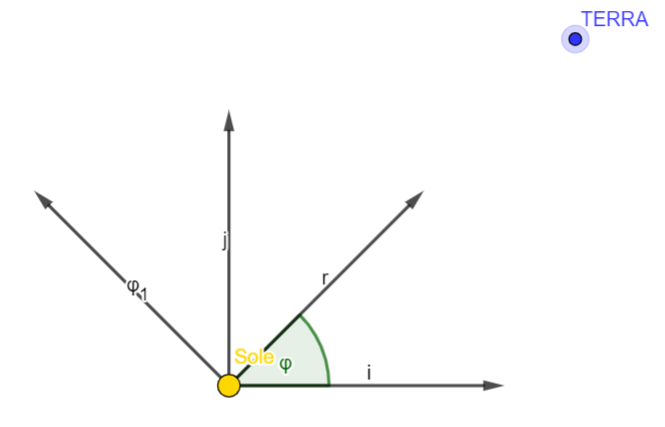
\includegraphics[width=0.4\linewidth]{polarcoordinates}
	\caption{Versori $\hat{i}$ e $\hat{j}$ cartesiani e versori posizione e angolo $\hat{r}$ e $\varphi$}
	\label{fig:polarcoordinates}
\end{figure}\\
In figura il vettore $\hat{\varphi}$, che si dovrebbe trovare applicato sul corpo in movimento, è stato traslato per rendere più chiari i passaggi ma ciò non cambia il livello concettuale di quanto faremo. \'{E} stato inoltre omesso il versore $\hat{k}$, che, come visto, è sempre costante.\\
Effettuare il passaggio in coordinate polari equivale ad esprimere i versori $\hat{r}$ e $\hat{\varphi}$ in funzione dei versori $\hat{i}$ e $\hat{j}$ e dell'angolo $\varphi$ (si noti che l'angolo $\varphi$ è uguale al modulo del vettore $\vec{\varphi}$). Per far ciò, come risulta evidente in figura, basta effettuare una rotazione dei versori $\hat{i}$ e $\hat{j}$ di un angolo $\varphi$. Per far ciò ci avvaliamo della matrice di rotazione
\begin{align*}
		\begin{pmatrix}
		\hat{r}\\
		\hat{\varphi}\\
		\hat{k}
	\end{pmatrix}=
	\begin{pmatrix}
		\cos\varphi&\sin\varphi&0\\
		-\sin\varphi&\cos\varphi&0\\
		0&0&1
	\end{pmatrix}
	\begin{pmatrix}
		\hat{i}\\
		\hat{j}\\
		\hat{k}
	\end{pmatrix}=
	\begin{pmatrix}
	\cos\varphi \hat{i} + \sin\varphi\hat{j}\\
	-sin\varphi \hat{i}+\cos\varphi\hat{j}\\
	\hat{k}
\end{pmatrix}\\\\
\end{align*}
Possiamo ora esprimere $\vec{r}$ e $\vec{v}$ in coordinate polari per poi calcolare il momento angolare.
\begin{align*}
&\frac{d\hat{r}}{dt} = \frac{d\hat{r}}{d\hat{\varphi}}\frac{d\hat{\varphi}}{dt} = \frac{d}{d\varphi}
\begin{pmatrix}
	\cos\varphi\hat{i}\\
	\sin\varphi	\hat{j}\\
	0
\end{pmatrix}
\dot{\varphi} = 
\begin{pmatrix}
	-\sin\varphi\hat{i}\\
	\cos\varphi	\hat{j}\\
	0
\end{pmatrix}
\dot{\varphi} = \dot{\varphi}\hat{\varphi}\\ \nonumber
&\frac{d\hat{\varphi}}{dt} = \frac{d\hat{\varphi}}{d\varphi}\frac{d\varphi}{dt} = \begin{pmatrix}
	-\cos\varphi\hat{i}\\
	-\sin\varphi	\hat{j}\\
	0
\end{pmatrix} \dot{\varphi} = -\dot{\varphi}\hat{r}\\ \nonumber
&\vec{r}= r\hat{r} 
\end{align*}
\begin{align}\label{eq:velocitàgravitazionale}
&\vec{v} \equiv\frac{d\vec{r}}{dt}=\frac{d}{dt}(r\hat{r})=\frac{dr}{dt}\cdot \hat{r} + r\cdot \frac{d\hat{r}}{dt} = \dot{r}\hat{r} + r\dot{\varphi}\hat{\varphi}
\end{align}
\begin{align}\label{eq:momentoangolaregravitazionale}
&\vec{L} = \mu\vec{r} \times \vec{v} = \mu \vec{r} \times (\dot{r}\hat{r}+r\dot{\varphi}\hat{\varphi})=\mu r\dot{r}(\hat{r}\times\hat{r})+ \mu\dot{\varphi}r^2(\hat{r}\times\hat{\varphi}) = \mu\dot{\varphi}r^2 \hat{k} 
\end{align}
Da quanto visto in precedenza, sappiamo che il momento angolare è costante in modulo direzione e verso, dunque non solo il versore $\hat{k}$ è costante nel tempo e quindi le orbite sono piane, ma sappiamo anche che il modulo $\mu\dot{\varphi}r^2$ è costante nel tempo, nonostante sia $r$ che $\dot{\varphi}$ cambino nel tempo. Questo vuol dire che essi variano insieme in modo da mantenere il prodotto $\dot{\varphi}r^2$ costante. Vedremo l'importanza di ciò nella deduzione della seconda legge di Keplero. Per stimare il valore del momento angolare possiamo calcolalo al perielio in cui la componente della velocità è solamente tangenziale; il modulo della distanza terra sole in questo punto è calcolabile con osservazioni astronomiche mentre la velocità semplicemente uguagliando forza centripeta e forza di attrazione gravitazionale in quel punto. \\\\\\
La seconda parte della prima legge di Keplero afferma che le orbite dei pianeti sono ellittiche e il sole giace sempre in uno dei suoi fuochi. Per una breve introduzione alle coniche si veda \ref{app:coniche}. Si ricordi  $\frac{d\hat{\varphi}}{dt} = -\dot{\varphi}\hat{r}$ ed $L = \mu r^2 \dot{\varphi}$.
\begin{align*}
	&\mu\frac{d^2\vec{r}}{dt^2} = \mu\frac{d\vec{v}}{dt} = -\frac{\alpha}{r^2}\hat{r} = \frac{\alpha}{r^2}\frac{1}{\dot{\varphi}} \frac{d\hat{\varphi}}{dt}\\ &\frac{d\vec{v}}{dt} = \frac{\alpha}{\mu r^2\dot{\varphi}} \frac{d\hat{\varphi}}{dt}= \frac{\alpha}{L}\frac{d\hat{\varphi}}{dt}\\
	&\frac{d}{dt}(\vec{v}-\frac{\alpha}{L}\hat{\varphi}) = 0 \\
	& \Rightarrow \vec{v}-\frac{\alpha}{L}\hat{\varphi} = \text{costante vettoriale}
\end{align*}
Dove, nel penultimo passaggio è stato sostituito il modulo del momento angolare, che come già visto è costante. Ricordiamo inoltre che la proprietà di costanza vettoriale implica che modulo, direzione e verso siano costanti nel tempo.\\
Come visto più volte in precedenza, la velocità è sempre perpendicolare alla traiettoria, essendone la derivata sul tempo, nel caso specifico del moto circolare risulta che la velocità è sempre perpendicolare anche al raggio vettore, cosa che però non è sempre vera per le ellissi. In questo caso infatti la velocità è perpendicolare sia al raggio che congiunge sole e pianeta, sia alla traiettoria, solamente in due punti particolari: l'afelio e il perielio, ovvero le intersezioni dell'asse maggiore con l'ellisse. Visto che la grandezza $\vec{v}-\frac{\alpha}{L}\hat{\varphi}$ è costante, potremo calcolarla nel punto della traiettoria in cui risulta più comodo, scegliamo il perielio. 
\begin{align*}
	&\vec{v}-\frac{\alpha}{L}\hat{\varphi} = \frac{L}{\alpha}\vec{v}-\hat{\varphi} = \frac{L}{\alpha}r\dot{\varphi} \hat{\varphi}-\hat{\varphi}= (\frac{L}{\alpha}r\dot{\varphi} -1)\hat{\varphi} = e\hat{j}
\end{align*}
Dove e è una costante con direzione $\hat{j}$ poiché $\hat{\varphi}$ è la direzione della velocità che nel perielio corrisponde con la direzione verticale (e deve rimanere costante). Procediamo ora con alcune manipolazioni algebriche
\begin{align*}
&(\frac{L}{\alpha}r\dot{\varphi} -1)\hat{\varphi}\cdot \hat{\varphi} = (e\hat{j})\cdot\hat{\varphi}\\
&\frac{L}{\alpha}r\dot{\varphi} -1 = e \cdot (-\sin\varphi\hat{i}+\cos\varphi\hat{j})\cdot\hat{j}= e \cos\varphi\\
&\frac{L}{\alpha} r \frac{r}{r} \dot{\varphi} \frac{\mu}{\mu} - 1 = \frac{L^2}{\alpha \mu r}-1 = e \cos\varphi\\
\end{align*}
\begin{align}\label{eq:conica}
	&r = \frac{L^2}{\alpha\mu}\frac{1}{e\cos\varphi+1}\quad \Rightarrow \text{Conica}
\end{align}
Quest'ultima è la forma generale delle coniche, il tipo di conica dipende dalla costante e, che a sua volta, come vedremo nella sezione (\ref{sec:energiasistema2corpi}), dipende dall'energia del sistema. Le osservazioni sperimentali di Keplero sono limitate ai pianeti del sistema solare, in cui e assume valori tali da avere sempre orbite ellittiche. Ciò che abbiamo appena ottenuto non è altro che una generalizzazione di quanto osservò Keplero: possiamo riformulare la terza legge, estendendola, come:\\
\textit{Sotto l'effetto di forza gravitazionale la traiettoria di un corpo attorno ad un altro descrive sempre una conica, in caso di orbita ellittica e se la massa di un corpo è trascurabile rispetto a quella dell'altro, allora il corpo con massa maggiore occupa uno dei fuochi dell'ellisse}.
\subsubsection{Seconda legge}
La seconda legge di Keplero dice che aree uguali sono spazzate in tempi uguali, ciò equivale a dire che la derivata sul tempo dell'area spazzata è costante. Cominciamo con il calcolare la spazzata d'area infinitesima $dA$, l'aera è contenuta in un settore circolare che però può essere visto come un triangolo per aree molto piccole perché un segmento rettilineo approssima bene una sezione di curva infinitamente piccola. L'area infinitesima del triangolo compreso fra i vettori posizione della terra $\vec{r}_1$ e $\vec{r}_2$ in due istanti di tempo infinitamente vicini (e quindi $\vec{r}_1=\vec{r}_2$), e di base $\vec{r}_1-\vec{r}_2 = d\vec{r}$ è calcolabile come 
\begin{align*}
	&dA = \frac{1}{2}|\vec{r}_1\times d\vec{r}|=\frac{1}{2}d\vec{r}(\vec{r}_1 \cdot \sin\theta)
\end{align*}
Dove $\theta$ è l'angolo compreso fra la base e l'altezza; questa formula equivale proprio alla classica $\frac{1}{2}\  base \cdot altezza$.
Sappiamo inoltre che $\vec{v}\equiv \frac{d\vec{r}}{dt}$ dunque $d\vec{r} = \vec{v}\cdot dt$. Calcoliamo ora l'area infinitesima $dA$ operando alcune manipolazioni algebriche e sostituzioni
\begin{align*}
&dA = \frac{1}{2}|\vec{r}\times( \vec{v}\cdot dt)|\\
&\frac{dA}{dt} =\dot{A} = \frac{1}{2\mu}\mu|\vec{r}\times \vec{v}|= \frac{|\mu \vec{r}\times \vec{v}|}{2\mu}= \frac{|\vec{L}|}{2\mu}= \frac{\mu r^2\dot\varphi}{2\mu}=\frac{r^2\dot\varphi}{2} \\
\end{align*}
Abbiamo già visto nella deduzione della prima legge di Keplero, che questa quantità è costante dunque la variazione dell'area spazzata nel tempo è costante: aree uguali sono spazzate in tempi uguali!
\subsubsection{Terza legge}\label{sec:terzalegge}
La terza legge di Keplero afferma che il rapporto fra semiasse maggiore al cubo e periodo di rivoluzione al quadrato è una costante per ogni pianeta del sistema solare:$\frac{a^3}{T^2}$ = costante. Calcoliamo per ora un'approssimazione per orbite circolari (le orbite dei pianeti del sistema solare sono effettivamente sono ellissi con eccentricità molto basse), la forma corretta verrà dedotta in seguito (sezione(\ref{sec:terzaleggerivista})). L'accelerazione centripeta nel caso di moto circolare è proprio la forza di attrazione gravitazionale. Il semiasse maggiore (uguale a quello minore nel cerchio), sarà uguale al raggio: $a = r$.
\begin{align*}
	&\vec{F}_c = \mu\frac{d^2\vec{r}}{dt^2}= -\mu\omega^2 r \hat{r} = -G\frac{Mm}{r^2} \hat{r}=\vec{F}_g\\
	&\omega =\frac{2\pi}{T}\\
	&\mu\frac{4\pi^2}{T^2} r  = G\frac{Mm}{r^2}\\
	&\frac{r^3}{T^2} = G\frac{Mm}{4 \mu \pi^2}= G\frac{Mm}{4 \pi^2 (\frac{Mm}{m+M})}= G\frac{M+m}{4 \pi^2} = \text{costante}
\end{align*} 
Questa legge è molto importante poiché permette di calcolare la massa del sole conoscendo il periodo di rivoluzione della terra (un anno) la costante di gravitazione universale, la massa della terra (già ottenute nelle sezioni precedenti) e la distanza terra-sole, calcolata da Edmond Halley (1656-1742), contemporaneo e conoscente di Newton, con considerazioni sulla prospettiva.
\begin{align*}
	&r_{ts} = 152\ 104\ 285\ 000\ m
	&M_s = \frac{r_{ts}^3\ 4 \pi^2}{T_t^2 G}m_t= 1,989 \cdot 10 ^{30} \ kg
\end{align*}
\subsection{Energia del sistema a due corpi e traiettoria ellittica}\label{sec:energiasistema2corpi}
Dalla geometria sappiamo che un'ellisse è caratterizzata da alcuni parametri:
\begin{itemize}
\item a = semiasse maggiore
\item b = semiasse minore
\item A = area = $\pi a b$
\item e = eccentricità = $\sqrt{1-\frac{b^2}{a^2}}$
\end{itemize}
Nel caso dell'orbita dei pianeti del sistema solare (ma più ingenerale, ogni volta che $M >> m$) risulta che
\begin{align*}
&2a = r_p+r_a\\
&r_p = \frac{L^2}{\alpha\mu}\frac{1}{1+e} \quad r_a = \frac{L^2}{\alpha\mu}\frac{1}{1-e}\\
&a = \frac{L^2}{\alpha\mu}\frac{1}{1-e^2}\\
\end{align*}
Dove $r_p$ è la distanza pianeta-sole all'afelio ed $r_a$ al perielio i cui valori ottenuti provengono dalla (\ref{eq:conica}). Abbiamo già visto che il momento angolare si conserva; la seconda grandezza conservata, essendo il sistema isolato e soggetto solamente a forze conservative, è l'energia meccanica totale (si veda (\ref{sec:energiapotenziale})). L'energia meccanica totale dei sistemi a due corpi appena visti risulta, come sempre, dalla somma di energia cinetica e potenziale
 \begin{align*}
 	E_m=\frac{1}{2}\mu v^2 - U(r) = \frac{1}{2}\mu v^2 -\frac{GMm}{r} = \frac{1}{2}\mu v^2 -\frac{\alpha}{r}
 \end{align*}
Dove U(r), l'energia potenziale, è quella potenziale gravitazionale, come visto in (\ref{sec:forzecentrali}).\\
Ricordando l'espressione della velocità (\ref{eq:velocitàgravitazionale}) sostituiamo
\begin{align*}
	&E_m= \frac{1}{2}\mu (\dot{r}\hat{r}+r\dot{\varphi}\hat{\varphi})^2 -\frac{\alpha}{r}= \frac{1}{2}\mu \dot{r}^2+ (\frac{1}{2}\mu r^2\dot{\varphi}^2 -\frac{\alpha}{r})
\end{align*}
Ricordando il modulo del momento angolare ricavato in (\ref{eq:momentoangolaregravitazionale}) sostituiamo nel secondo addendo
\begin{align*}
	&L = \mu r^2 \dot{\varphi}\\
	&E_m= \frac{1}{2}\mu \dot{r}^2+ (\frac{L^2}{2\mu r^2} -\frac{\alpha}{r})
\end{align*}
Essendo l'energia costante, calcoliamola nel punto in cui ci risulta più facile: il perielio. In questa posizione, come già notato, la componente $\dot{r} = 0$, dunque l'energia si semplifica in
\begin{align*}
	&E_m= \frac{L^2}{2\mu r_p^2} -\frac{\alpha}{r_p}
\end{align*}
Sostituiamo il valore di $r_p$ e svolgiamo alcuni passaggi algebrici
\begin{align}\label{eq:eccentricità}
	&E_m=\frac{L^2}{2\mu (\frac{L^2}{\alpha\mu}\frac{1}{1+e})^2} -\frac{\alpha}{(\frac{L^2}{\alpha\mu}\frac{1}{1+e})} = \frac{\alpha^2 \mu}{2L^2}(e^2-1)\\ \nonumber
	&e = \sqrt{1+\frac{2EL^2}{\mu\alpha^2}}
\end{align}
Ecco ricavata la costante $e$, ne segue che l'eccentricità della conica che descrive la traiettoria dipende dall'energia meccanica del sistema! In particolare, se $E< 0$ si ha un'ellisse, se $E = 0$ una parabola e se $E >0$ un'iperbole. Infatti, essendo l'orbita dei pianeti del sistema solare ellittica, per le proprietà di questa figura geometrica abbiamo $0<e<1$, da cui ne segue che l'energia ha segno negativo. Possiamo dunque scrivere
\begin{align*}
&-|E| = \frac{\alpha^2 \mu}{2L^2}(e^2-1)\\
&|E| = \frac{\alpha^2 \mu}{2L^2}(1-e^2)
\end{align*} 
Ora, conoscendo il valore di a, ricavato a inizio sezione, sostituiamola in quest'ultima espressione dell'energia. 
\begin{align*}
& E = -\frac{\alpha}{2a}\\
& a = \frac{\alpha}{2|E|}
\end{align*}
Ecco ricavato che il semiasse maggiore dipende dall'energia meccanica del sistema. Il semiasse maggiore però non basta per identificare l'ellisse descritta dalla traiettoria, infatti esistono infinite ellissi con il medesimo semiasse maggiore (e quindi con la stessa energia).\\
\begin{figure}[h!]
	\centering
	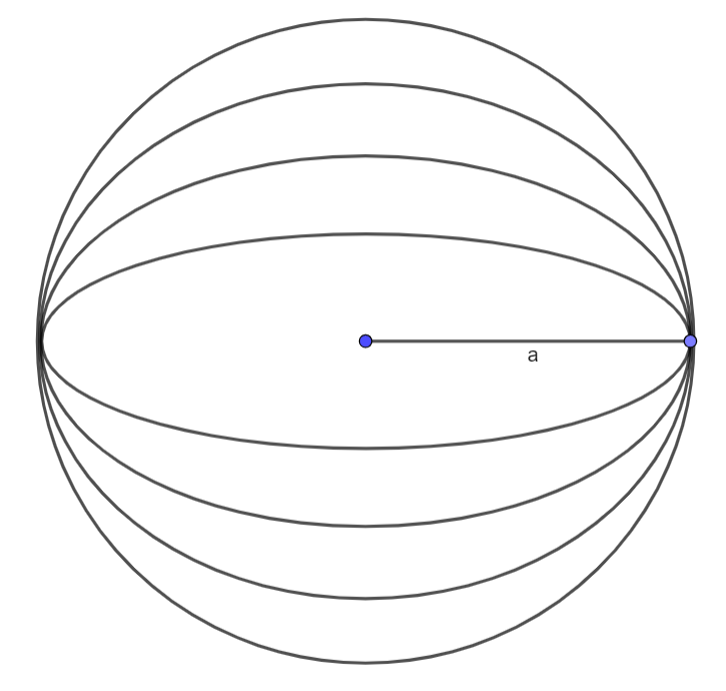
\includegraphics[width=0.3\linewidth]{molte_ellissi}
	\caption{Infinite traiettorie ellittiche sono associate ad un unico valore di energia meccanica totale del sistema. Per individuare un'unica ellisse non basta solamente il semiasse maggiore.}
	\label{fig:molteellissi}
\end{figure}\\
Per individuare un'unica ellisse ci occorre stabilire anche un valore per il semiasse minore $b$.
Per farlo, eguagliamo la (\ref{eq:eccentricità}) con la definizione di eccentricità vista a inizio paragrafo, in cui sostituiamo il valore di $a$ ottenuto.
\begin{align*}
	&e = \sqrt{1-\frac{b^2}{a^2}} = \sqrt{1-\frac{b^24E^2}{\alpha^2}} = \sqrt{1+\frac{2|E|L^2}{\mu\alpha}}\\
	&b = \frac{L}{\sqrt{2\mu|E|}}
\end{align*}
Il semiasse minore dipende sia dall'energia del sistema sia dal suo momento angolare (l'altra grandezza costante) ne deduciamo che per determinare la traiettoria di un pianeta necessitiamo solamente dei valori costanti di energia meccanica e momento angolare. 
\subsection{La terza legge di Keplero rivista}\label{sec:terzaleggerivista}
Una volta acquisite queste conoscenze, possiamo rivedere le tre leggi di Keplero sotto una diversa luce. In particolare vogliamo ricavare la terza legge di Keplero a partire dalle prime due, evitando l'approssimazione ad orbite circolari. Partiamo dalla seconda legge
\begin{align*}
	&\frac{dA}{dt} = \text{costante} = \frac{|\vec{L}|}{2\mu}\\
	&\int\frac{dA}{dt}dt = \int\frac{|\vec{L}|}{2\mu}dt\\
	&\int_0^{2\pi} dA = \int_0^T\frac{|\vec{L}|}{2\mu}dt\\
	&\pi a b = \frac{|\vec{L}|}{2\mu} \cdot T
\end{align*}
Dove il primo membro è l'area dell'ellisse e il secondo il periodo di rivoluzione.\\
Ora eleviamo al quadrato entrambi i membri, sostituiamo b e svolgiamo qualche passaggio algebrico.
\begin{align*}
	&\pi^2 a^2 (\frac{L}{\sqrt{2\mu |E|}})^2  = (\frac{|\vec{L}|}{2\mu})^2 \cdot T^2\\
	&\pi^2 a^2(\frac{\alpha}{2|E|})=\frac{\alpha T^2}{4 \mu}\\
\end{align*}
Sostituiamo il valore di a ottenuto in precedenza. 
\begin{align*}
	&\pi^2 a^3=\frac{\alpha T^2}{4\mu} = \frac{GMm T^2}{4}\frac{M+m}{Mm}\\
	&\frac{a^3}{T^2}=\frac{G(M+m)}{4\pi^2}
\end{align*}
Che è la forma corretta per orbite ellittiche della sezione (\ref{sec:terzalegge}). Notiamo che le due forme sono identiche a meno del raggio, sostituito dal semiasse maggiore.
\subsection{Generalizzazione del rapporto tra energia e traiettoria}
Prendiamo in considerazione l'espressione dell'energia meccanica ottenuta
\begin{align*}
	&E_m= \frac{1}{2}\mu \dot{r}^2+ (\frac{L^2}{2\mu r^2} -\frac{\alpha}{r})
\end{align*}
Notiamo che questa formula presenta un primo addendo che varia con la velocità, mentre un secondo e terzo addendo che dipendono unicamente dalla distanza, caratteristica fondamentale dell'energia potenziale a cui "assomigliano". Diciamo che questi ultimi due formano l'\textbf{energia potenziale efficace} $U_{eff}$.
\begin{align*}
&U_{eff}(r) = \frac{L^2}{2\mu r^2} -\frac{\alpha}{r}
\end{align*}
Questa è formata da un termine repulsivo, con segno sempre positivo (o al massimo nullo per $L=0$) e dipendente da $\frac{1}{r^2}$ (tutto il resto è costante) ed un termine di segno sempre negativo e quindi attrattivo, dipendente da $\frac{1}{r}$. Potendo essere sia negativa che positiva, l'energia potenziale efficace determina il segno dell'energia meccanica.  Risulta utile studiare le proprietà dell'energia potenziale efficace, in riferimento al suo grafico, considerando due casi: $L=0$ ed $L>0$.
\newpage
\subsubsection*{Orbite coniche non degeneri: L > 0}
In questo caso, visto che $L = \mu r^2 \dot{\varphi} \sin(\theta) =  \mu r v \sin(\theta) $ ne deduciamo che $\dot{\varphi}\neq 0$, dunque il moto è affetto da una rotazione e, come dimostrato, descrive una conica. Inoltre possiamo individuare il valore $b$, detto \textbf{parametro d'impatto} che rappresenta la minima distanza tra il sole (corpo di massa M) e la retta che percorrerebbe un corpo di massa m, senza l'influenza dell'attrazione del sole.
\begin{figure}[h!]
	\centering
	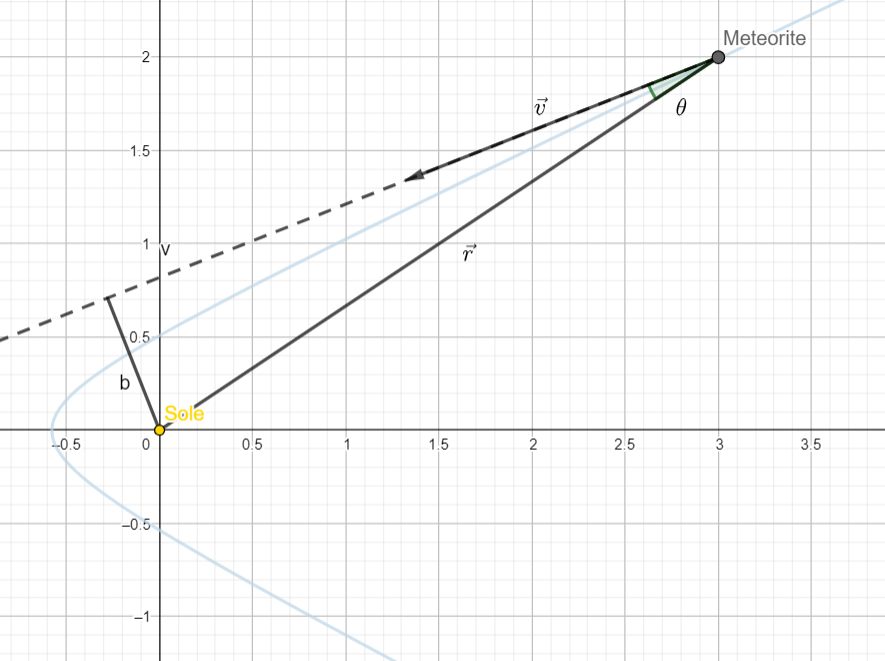
\includegraphics[width=0.5\linewidth]{meteorite}
	\caption{Grafico esplicativo del parametro d'impatto}
	\label{fig:meteorite}
\end{figure}\\
Si noti che, essendo $L$ costante e diverso da zero per ipotesi, il valore di $b$ non può raggiungere zero, a meno che non vi siano forze esterne non conservative come l'attrito (caso che tratteremo più avanti), un meteorite dunque non può cadere sulla terra in una condizione del genere se approssimiamo i corpi come puntiformi. Se invece il corpo ha un raggio diverso da zero avremo che l'impatto avviene se il raggio è maggiore del parametro d'impatto.\\
Ora, riferendoci al grafico, svolgiamo alcune considerazioni sul segno di $U_{eff}$ e quindi su quello di $E_m$, per poi ricavare informazioni generali sul moto del corpo. Visto che l'energia è costante e al perielio è uguale all'energia potenziale efficace, per determinare il segno dell'energia basterà studiare la curva di $U_{eff}$.\\
\begin{figure}[h!]
	\centering
	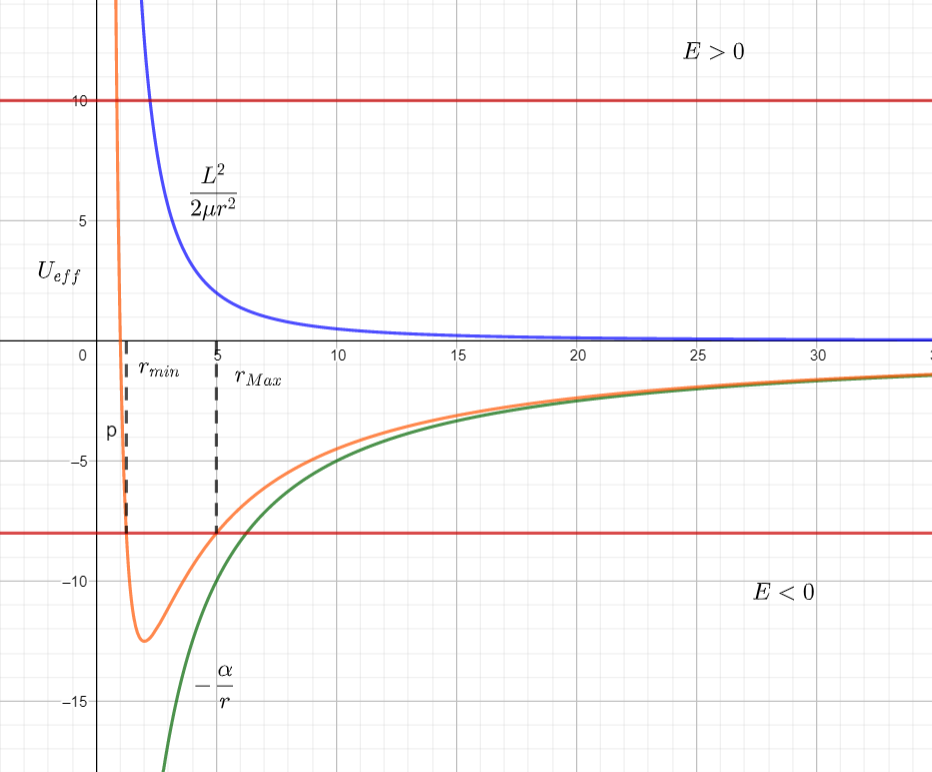
\includegraphics[width=0.5\linewidth]{potenziale_efficace}
	\caption{Grafico qualitativo delle due componenti del potenziale efficace (blu e verde) e del potenziale efficace (arancione). Sull'asse x i valori di r, sulle y $U_{eff}$}
	\label{fig:potenzialeefficace}
\end{figure}\\
Possiamo distinguere tre casi, a seconda del valore che assume l'energia. Per $r$ piccoli, domina il termine positivo, $U_{eff}$ è positiva e dunque $E > 0$. La retta dell'energia (costante)  interseca $U_{eff}$ in un solo punto, che è la distanza minima possibile tra i due corpi. Riferendosi all'espressione dell'eccentricità in funzione dell'energia, si ha che la traiettoria descritta è iperbolica. Se $E = 0$ invece l'orbita è parabolica (il valore minimo di E per cui si interseca una sola volta $U_{eff}$). Se invece l'energia è minore di zero, la retta intersecherà la curva in due punti: $r_{min}$ ed $r_{max}$, ovvero i punti entro i quali è contenuta la traiettoria del corpo, che evidentemente sarà ellittica. Infine, quando la retta $E<0$ interseca $U_{eff}$ nel suo punto inferiore, quando $U_{eff}$ è minima, si ha che $r_{min}=r_{max}$, ovvero un'orbita circolare. 
\subsubsection*{Il caso limite, le orbite degeneri: L = 0}
Se $L=0$, ricordando $L = \mu r^2 \dot{\varphi}$, ne segue che $\dot{\varphi} = 0$ (non ha senso che massa e raggio siano nulli). Ricordiamo che $\dot{\varphi}$ rappresenta la velocità angolare; essendo nulla il moto del corpo è radiale, cioè si muove in linea retta attratto da un'altro corpo.
In questo caso la prima componente si annulla e $U_{eff} = \frac{-\alpha}{r}$.
\begin{figure}[h!]
	\centering
	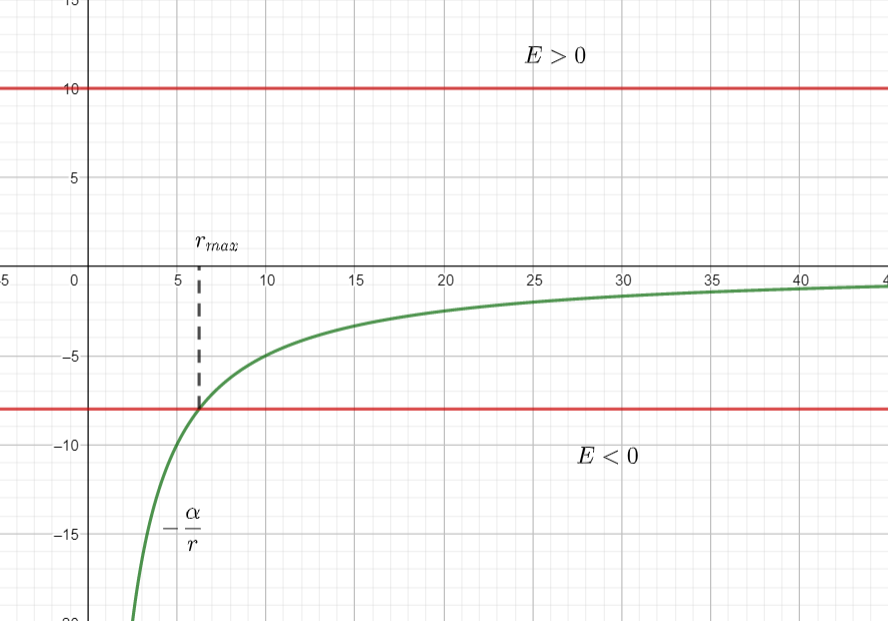
\includegraphics[width=0.5\linewidth]{U_eff1}
	\caption{Grafico qualitativo dell'energia potenziale efficace per $L=0$.}
	\label{fig:ueff1}
\end{figure}
Se l'energia è positiva, il termine $\frac{1}{2}\mu \dot{r}^2$ avrà prevalso su $U_{eff}$, dal grafico notiamo che la retta dell'energia (parallela all'asse x poiché costante) non interseca mai la curva dell'energia potenziale, ciò vuol dire che la distanza $r$ fra i due corpi può assumere qualsiasi valore positivo. In termini pratici, il corpo si muove in linea retta e, se ha velocità negativa (in direzione dell'altro corpo), allora vi si scontrerà, se invece ha velocità positiva (si sta allontanando dall'altro corpo, come se stessimo lanciando un sasso dalla terra verso fuori) allora il corpo si allontanerà all'infinito; in ognuno dei due casi la distanza fra i due corpi può assumere qualsiasi valore positivo.\\
Se l'energia è nulla e la velocità negativa, il corpo cade sull'altro, se invece la velocità è positiva, il corpo ha l'energia minima per allontanarsi dall'altro corpo all'infinito, lo farà dunque con la minima velocità possibile.\\
Se l'energia è negativa, la retta dell'energia interseca in un solo punto la curva di $U_{eff}$, ciò vuol dire che esiste un valore massimo di distanza che il corpo può raggiungere, in termini pratici, se la velocità ha verso positivo il corpo si allontana (sempre il linea retta) fino a raggiungere la distanza $r_{max}$ per poi tornare indietro con velocità cambiata di segno e colpire l'altro corpo. Il caso con energia negativa e verso positivo invece non è fisico perché è come se il corpo proveniente dall'infinito verso la terra la supera (assurdo) arriva ad una distanza massima e poi torna indietro.\\\\

Riassumendo, se $E \geq 0$, l'energia cinetica prevale su quella potenziale e il corpo meno massiccio scappa dall'orbita dell'altro, descrivendo traiettorie ellittiche (se $E \neq 0$), paraboliche (se $E = 0$) o rette, nel caso limite ($L= 0$), in cui come visto si può avere lo scontro dei due corpi. Se invece $E < 0$, prevale l'energia potenziale su quella cinetica, il corpo meno massiccio rimane bloccato nell'orbita dell'altro, descrivendo orbite ellittiche ($L \neq 0$) o, nel caso limite ($L= 0$), un segmento in cui si ha con certezza la collisione dei due corpi. 
\begin{figure}
	\centering
	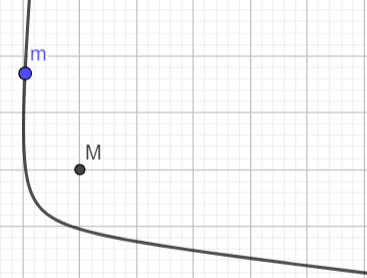
\includegraphics[width=0.175\linewidth, height=0.085\textheight]{iperbole} \quad
	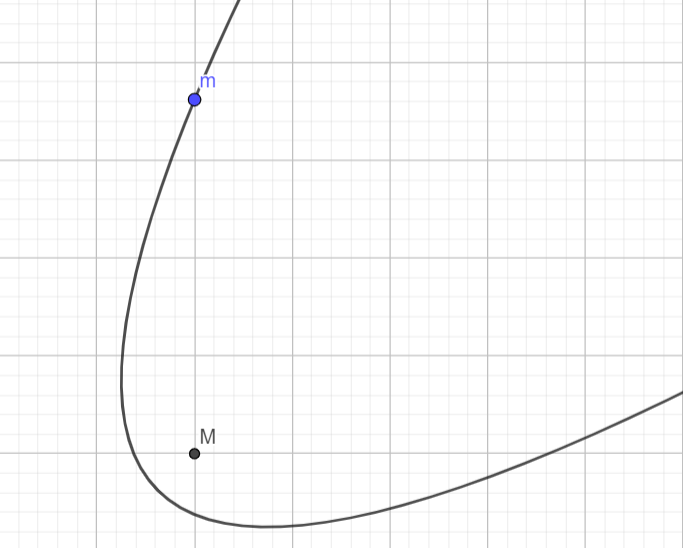
\includegraphics[width=0.175\linewidth, height=0.085\textheight]{parabola} \quad
	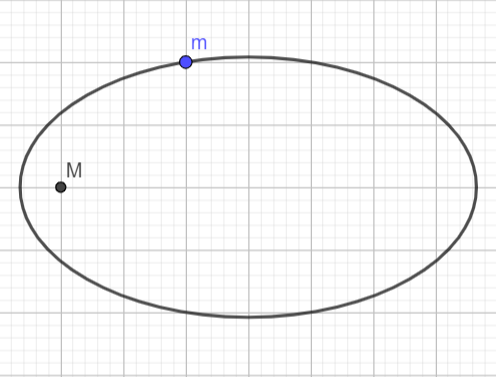
\includegraphics[width=0.175\linewidth, height=0.085\textheight]{ellipse} \quad
	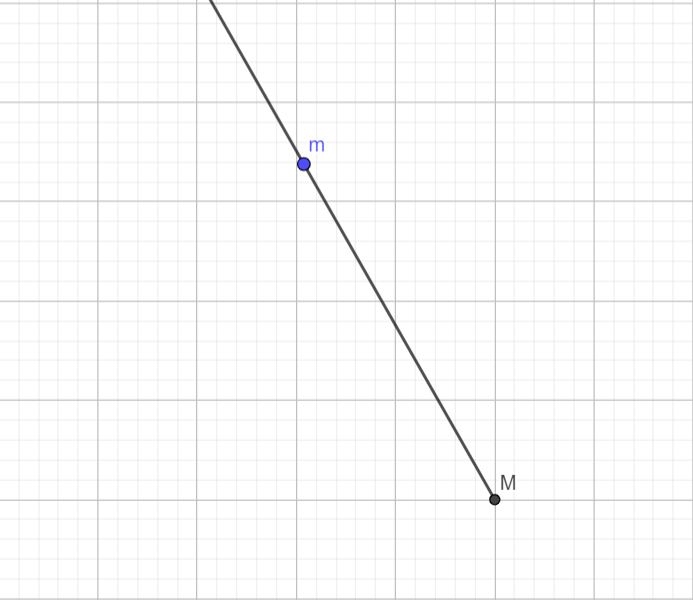
\includegraphics[width=0.175\linewidth, height=0.085\textheight]{semiretta} \quad 
	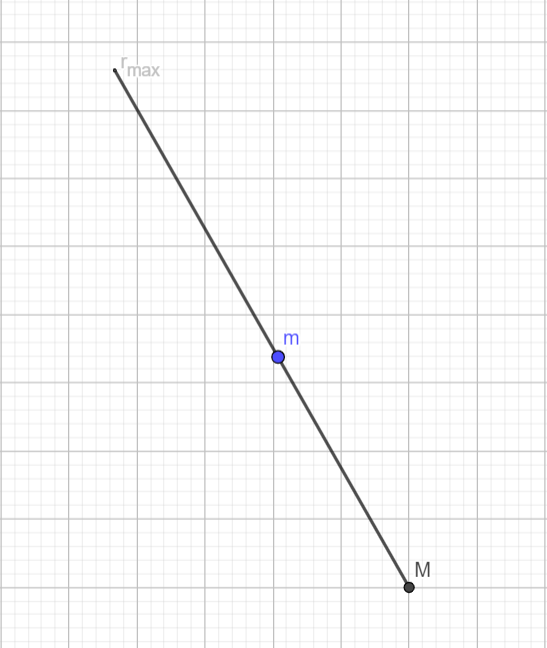
\includegraphics[width=0.175\linewidth, height=0.085\textheight]{Segment}
	\caption{Da sinistra: \newline 
$\begin{cases}
	E > 0\\
	L \neq 0\\
	r \in [r_{min}, +\infty]
\end{cases}$
$\begin{cases}
	E = 0\\
	L \neq 0\\
	r \in [r_{min}, +\infty]
\end{cases}$
$\begin{cases}
	E < 0\\
	L \neq 0\\
	r \in [r_{min}, r_{max}]
\end{cases}$
$\begin{cases}
	E \geq 0\\
	L = 0\\
	r \in [0, +\infty]
\end{cases}$
$\begin{cases}
	E < 0\\
    L = 0\\
   	r \in [0, r_{max}]
\end{cases}$
}
	\label{fig:parabola}
\end{figure}
\subsection{La collisione fra due corpi in orbita}
Abbiamo visto che nel caso in cui $L = 0$ o se il parametro d'impatto è minore del raggio, i due corpi collidono. L'eventualità che un corpo, come un meteorite, colpisca la terra è improbabile visto che il rapporto fra spazio vuoto e superficie terrestre è estremamente alto. Tuttavia esiste un'altro caso in cui due corpi possono collidere dovuto alla presenza di forze non conservative come quella d'attrito. Si consideri la seguente situazione: un corpo di massa m segue un'orbita ellittica attorno ad un'altro di massa M (con $M >> m$), durante la sua traiettoria entra in contatto con polveri e gas che generano attrito, l'energia meccanica è trasformata in calore e, dunque, dissipata ($\frac{dE}{dt}<0$). Inizialmente, essendo l'orbita ellittica e non degenere, abbiamo $E < 0$, $L\neq0$. Se però l'energia diminuisce nel tempo, ricordando la relazione fra energia e semiasse maggiore, avremo che l'energia varia in funzione di a ed a varia in funzione del tempo.
\begin{align*}
	&E(a) = -\frac{\alpha}{2a(t)}\\
	&\frac{dE(a)}{dt} = \frac{dE}{da}\frac{da}{dt} = \frac{\alpha}{2a^2} \frac{da}{dt}<0\\
	&\Rightarrow \frac{da}{dt} < 0
\end{align*}
Da ciò deriva che se l'energia diminuisce, allora il semiasse maggiore diminuisce. Dunque, per il limite $E\rightarrow -\infty$ si ha che $a\rightarrow 0$. Tuttavia, i sistemi reali sono formati da corpi non puntiformi, che hanno un raggio finito, quindi se l'energia tende ad un valore negativo molto basso (ma finito!), allora il semiasse maggiore dell'orbita assume un valore minore o uguale al raggio del pianeta; i due collideranno. 
\subsection{La dinamica di razzi}
Studiamo ora la dinamica dei razzi. per far ciò serve considerare la velocità del razzo rispetto alla piattaforma di lancio ($\vec{v}_{rp}$), la velocità del gas espulso dal razzo rispetto alla piattaforma ($\vec{v}_{gp}$) e rispetto al razzo ($\vec{v}_{gr}$). Bisogna inoltre tener conto che la massa del razzo non è costante nel tempo in quanto grandi quantità di carburante vengono consumate. 
\begin{align*}
	\sum_i &\vec{F}_i^{ext} = \frac{d\vec{p}}{dt}\\
	\vec{p}_i &= m \vec{v}_{rp}\\
	\vec{p}_f &= (m - dM) (\vec{v}_{rp}+d\vec{v}_{rp})+dM\vec{v}_{gp} = (m - dM) (\vec{v}_{rp}+d\vec{v}_{rp})+dM(\vec{v}_{rp}+\vec{v}_{gr})\\
	d\vec{p} &= \vec{p}_f - \vec{p}_i = (m - dM) (\vec{v}_{rp}+d\vec{v}_{rp})+dM(\vec{v}_{rp}+\vec{v}_{gr}) - m \vec{v}_{rp}=\\
	&m \vec{v}_{rp}+md\vec{v}_{rp}-dM \vec{v}_{rp}-dM d\vec{v}_{rp}+dM \vec{v}_{rp} + dM \vec{v}_{gr}-m\vec{v}_{rp}=\\ 
	&m d\vec{v}_{rp}+dM \vec{v}_{gr}-dM d\vec{v}_{rp}
\end{align*}
L'ultimo termine ottenuto contiene due differenziali, è quindi trascurabile rispetto alle altre grandezze: lo eliminiamo. La variazione di massa del gas espulso $dM$ (positiva perché aumenta) è uguale alla variazione di massa del razzo con segno negativo $-dm$ perché diminuisce. Sostituiamo e calcoliamo ora la derivata rispetto al tempo 
\begin{align*}
	dM &= -dm\\
	\frac{d\vec{p}}{dt} &= m \frac{d\vec{v}_{rp}}{dt} - \frac{dm}{dt} \vec{v}_{gr}\\
	\sum_i \vec{F}_i^{ext} &= m \frac{d\vec{v}_{rp}}{dt} - \frac{dm}{dt} \vec{v}_{gr}\\
	m \frac{d\vec{v}_{rp}}{dt} &= 	\sum_i \vec{F}_i^{ext} + \frac{dm}{dt} \vec{v}_{gr}
\end{align*}
La forza esterna che agisce sul razzo è quella di gravità mentre quella interna è la spinta, data dalla variazione della massa espulsa per la velocità a cui viene espulsa. Nello spazio la forza di gravità è trascurabile quindi la somma delle forze esterne è nulla.
\begin{align*}
	&m \frac{d\vec{v}_{rp}}{dt} = \frac{dm}{dt}\vec{v}_{gr} \rightarrow d\vec{v}_{rp} = \frac{dm}{m} \vec{v}_{gr}\\
	&\int d\vec{v}_{rp} = \int \frac{dm}{m} \vec{v}_{gr}\\
	&\vec{v}_{rp}(t)-\vec{v}_{rp}(0) = \vec{v}_{gr} \ln(\frac{m(t)}{m_0})
\end{align*}
Visto che il razzo e il gas si muovono nella stessa direzione ma con versi opposti, possiamo togliere i simboli di vettore ed aggiungere i segni appropriati. definendo come verso positivo quello in cui si muove il razzo otteniamo
\begin{align*}
&\vec{v}_{rp}(t) = \vec{v}_{rp}(0)+ \vec{v}_{gr} \ln(\frac{m(t)}{m_0})\\
&{v}_{rp}(t) = {v}_{rp}(0)- {v}_{gr} \ln(\frac{m(t)}{m_0})\\
&{v}_{rp}(t) = {v}_{rp}(0)+ {v}_{gr} \ln(\frac{m_0}{m_(t)})\\
\end{align*}
Quest'ultima è l'equazione del moto dei razzi nello spazio, da qui deriva una utile considerazione pratica: per aumentare la velocità del razzo è più vantaggioso aumentare la velocità di espulsione del gas o far variare la massa? Da questa equazione notiamo che la velocità del razzo aumenta proporzionalmente alla velocità di espulsione del gas mentre la variazione di massa è dentro il logaritmo, è più vantaggiosa la prima. 
\section{La dinamica dei corpi rigidi}
Come visto un corpo rigido ha 6 d.o.f., per descrivere il suo moto si usano le due equazioni cardinali della conservazione del momento angolare e della quantità di moto. Vogliamo studiare la relazione che sussiste tra $\vec{\omega}$ e $\vec{L}$.\\
Se ci spostiamo nel centro di massa abbiamo, per la quarta proprietà del centro di massa (sezione \textbf{\ref{sec:quartaprop}}), $\vec{L} = \vec{L}'$. consideriamo per semplicità il caso in cui la rotazione avvenga solamente rispetto all'asse z
\begin{align*}
	&\vec{\omega}=\omega \hat{k}\\
	&\vec{L}=\sum_i \vec{r}_i \times m_i \vec{v}_i
\end{align*} 
Quest'ultima espressione del momento angolare è valida solamente se il polo viene preso sull'asse di rotazione,questa forma risulta più semplice perché tutti i punti sull'asse di rotazione sono fermi.\\
\'{E} sempre possibile scrivere il vettore $\vec{r}_i$ come somma di un vettore sull'asse z e uno sull'asse x, perpendicolare a z
\begin{align*}
	\vec{r}_i = z_i \hat{k} + \vec{d}_i
\end{align*}
Qualunque sia la forma del corpo, un generico punto materiale di massa $m_i$ descriverà sempre una circonferenza di raggio $d_i$, si muoverà quindi di moto circolare. Possiamo esprimere il vettore $\vec{v}_i$ e sostituire nel momento angolare $\vec{L}$. 
\begin{align*}
	\vec{v}_i &= \vec{\omega}\times \vec{d}_i\\
	\vec{L} &= \sum_i \vec{r_i} \times m_i \vec{v}_i = \sum_i \vec{r_i} \times m_i (\vec{\omega}\times \vec{d}_i) = \sum_i m_i[\vec{\omega}(\vec{r_i}\vec{d}_i)-\vec{d}_i(\vec{r_i}\vec{\omega})]= \\
	& \sum_i m_i[\vec{\omega}((z_i \hat{k} + \vec{d}_i)\vec{d}_i)-\vec{d}_i((z_i \hat{k} + \vec{d}_i)\vec{\omega})]=\\
	&\sum_i m_i[\omega \hat{k}(d_i z_i (\hat{i} \cdot \hat{k})+d_i^2(\hat{i}\cdot \hat{i}))-d_i \hat{i}(z_i \omega (\hat{k} \cdot \hat{k})+ d_i \omega (\hat{i}\cdot \hat{k}))]=\\
	&\sum_i m_i[\omega \hat{k}(d_i^2)-d_i \hat{i}(z_i \omega)] = \sum_i m_i \omega d_i^2 \hat{k} - \sum_i m_i d_i z_i \omega \hat{i}=\\
	& \sum_i m_i d_i^2 \vec{\omega}- \sum_i z_i m_i \omega \vec{d}_i 
\end{align*} 
Il primo termine di quest'ultima espressione dipende unicamente dalle caratteristiche del corpo (massa e forma) e della velocità angolare, definiamo il \textbf{momento d'inerzia} I come
\begin{align*}
	I \equiv \sum_i m_i d_i^2
\end{align*}
Risulta chiaro che I è una grandezza scalare e la sua unità di misura è $kg \cdot m^2$. Riscriviamo $\vec{L}$
\begin{align*}
&\vec{L} =  I \vec{\omega} - \sum_i z_i m_i \omega \vec{d}_i 
\end{align*} 
Il secondo membro è piuttosto complesso ma è spesso molto minore del primo poiché i $\vec{d}_i$ possono essere sia positivi che negativi, e per questo tendono a cancellarsi. Immaginiamo di calcolare il momento di inerzia di una pietra irregolare presa in spiaggia, il secondo membro tenderà statisticamente a zero. Per le stesse ragioni, il secondo membro si annulla se il corpo presenta una simmetria di rotazione rispetto all'asse di rotazione e quindi rispetto al polo scelto visto che lo abbiamo preso sull'asse.\\
Un corpo gode di \textbf{simmetria di rotazione} se per ogni massa $m_i$ a distanza $\vec{d}_i$ esiste un'altra massa equivalente posta a distanza $-\vec{d}_i$. In questo caso il secondo membro si annulla perché i termini positivi e negativi della sommatoria si eguagliano.\\
Per semplicità consideriamo solamente corpi con simmetria di rotazione e che ruotano attorno all'asse z, il momento angolare si ridurrà a
\begin{align*}
	&L_z = I \omega_z \\
	&\frac{d L_z}{dt} = \frac{d(I \omega_z)}{dt} = I \dot{\omega} = \tau_z
\end{align*}
Si noti la bella analogia fra forza, uguale a massa inerziale per accelerazione lineare e momento della forza, uguale a momento d'inerzia per accelerazione angolare. il momento d'inerzia è l'analogo rotazionale della massa inerziale: è una grandezza che indica quanto il corpo si oppone alle rotazioni.\\
Un classico esempio utile per la comprensione della relazione sussistente tra momento d'inerzia e momento angolare è quello della pattinatrice su ghiaccio che effettua una piroetta. Il corpo umano presenta una simmetria rotazionale (a grandi linee) quindi il momento angolare solamente uguale al momento d'inerzia per la velocità angolare. Sappiamo inoltre che in natura il momento angolare è sempre conservato. Se la ballerina comincia a ruotare attorno al suo asse di simmetria, considerando gli attriti trascurabili, con le braccia distese lungo i fianchi avrà un certo momento di inerzia e una velocità angolare. Se durante la rotazione allarga le braccia, ci sarà della massa che ora è posta ad una distanza maggiore dall'asse di rotazione rispetto alla condizione iniziale, dunque il momento d'inerzia aumenterà. Se il momento angolare deve rimanere costante e il momento d'inerzia aumenta, allora la velocità angolare deve diminuire. Questo è ciò che si ammira spesso durante le gare di pattinaggio di figura. 
\subsection{Teorema di Huygens-Steiner o degli assi paralleli}
Abbiamo visto fin'ora come calcolare il momento d'inerzia di sistemi rispetto al centro di massa, posto sull'asse di rotazione. Grazie a questo teorema è possibile ricavare il momento di inerzia rispetto a qualsiasi asse parallelo a quello calcolato rispetto all'asse passante per il centro di massa. Vediamo come ricavare questo importante risultato. 
\begin{align*}
	I_{cm} &= \sum_i m_i r'^2_i = \sum_i m_i (\vec{r}_i-\vec{r}_{cm})^2 =\\
	& \sum_i m_i r_i^2 + \sum_i m_i r_{cm}^2 -2\sum_i m_i \vec{r}_i\cdot \vec{r}_{cm} =\\
	&I + M r_{cm}^2 -2 \frac{M}{M} \sum_i m_i \vec{r}_i\cdot \vec{r}_{cm} =\\
	&I + M r_{cm}^2 -2 M \vec{r}_{cm}^2 = I - M r_{cm}^2\\
	\Rightarrow & I = I_{cm} +  M r_{cm}^2
\end{align*}
dove M è la massa dell'intero sistema ed $\vec{r}_{cm}$ è la distanza del nuovo asse dal centro di massa. 
\subsection{Il momento d'inerzia di figure semplici}
La definizione data di momento d'inerzia si riferisce a sistemi discreti di punti materiali, se però il nostro corpo è formato da infiniti punti materiali, analogamente a quanto fatto per il centro di massa, è possibile effettuare il passaggio al continuo, sostituendo l'integrale alla sommatoria. 
\begin{align*}
	&I \equiv \int_M r^2 dm
\end{align*}
Come vedremo, per la risoluzione degli integrali specifici si effettua sempre una sostituzione della massa con la densità lineare, di superficie o volumica per la lunghezza, superficie o volume, in modo da poter risolvere l'integrale.
\subsubsection*{Disco}
Per il calcolo di quest'integrale sostituiamo dm con la massa di una corona circolare di spessore infinitesimo.
\begin{align*}
	&\rho_s = \frac{M}{\pi r^2} \quad dm = \rho_s 2 \pi r dr \\
	&I = \int r^2 dm = \int r^2 \rho_s 2\pi r dr = \rho_s 2\pi \int r^3 dr = \frac{M}{\pi r^2} 2\pi \frac{r^4}{4} = \frac{M r^2}{2}  
\end{align*}
\subsubsection*{Cilindro}
Sostituiamo dm con la massa di un toroide di rotazione di spessore infinitesimo.
\begin{align*}
	&\rho_v = \frac{M}{\pi r^2 h} \quad dm = \rho_v 2 h \pi r dr\\
	&I = \int r^2 dm = \int r^2 \rho_v 2 h \pi r dr = \rho_v 2 h \pi \frac{r^4}{4}= \frac{M}{\pi r^2 h} 2 h \pi \frac{r^4}{4} = \frac{M r^2}{2}
\end{align*}
\subsubsection*{Sbarra}
In questo caso vogliamo calcolare sia il momento d'inerzia relativo al centro di massa, sia quello relativo ad un'estremità in quanto in molte applicazioni si trova un'asta vincolata ad un'estremità che ruota. Cominciamo con il calcolo rispetto ad un'estremità, sostituiamo dm con la massa di una porzione infinitesima di sbarra. 
\begin{align*}
	&\rho_l = \frac{M}{r} \quad dm = \rho_r dr\\
	&I = \int r^2 dm = \int r^2 \rho_r dr = \rho_r \frac{r^3}{3} = \frac{M r^2}{3}
\end{align*}
Sfruttiamo ora il teorema di Huygens-Steiner per calcolare $I_{cm}$, il centro di massa si trova a metà della sbarra, quindi $d = r/2$.
\begin{align*}
	&I_{cm} = I - M d^2 = \frac{M r^2}{3} - M (\frac{r}{2})^2 = \frac{M r^2}{12}
\end{align*}
\subsubsection{Esempio di applicazione}
Si consideri una sbarra con momento d'inerzia I, centro di massa C e lunghezza l, sospesa nel vuoto in assenza di attrito. Se si esercita una forza perpendicolare alla sbarra su un punto della sbarra, per un certo intervallo di tempo (impulso), a distanza d dal suo centro di massa si creerà un momento della forza che genererà una rotazione
\begin{align*}
	\vec{\tau} = \vec{d}\times\vec{F} = d \cdot F \hat{k}
\end{align*} 
Notiamo che se l'impulso fosse stato applicato al centro di massa il momento della forza sarebbe stato nullo e la sbarra si sarebbe mossa semplicemente di moto rettilineo uniforme. Sorge spontanea una domanda: attorno a quale punto ruota la sbarra? Supponiamo per assurdo che non ruoti attorno al centro di massa ma attorno ad un qualsiasi altro punto, ne risulterebbe che il centro di massa comincerebbe a rototraslare in modo molto complesso. Questo è assurdo perchè sappiamo che il centro di massa si deve comportare come un punto materiale in cui è concentrata l'intera massa dell'aggetto, un punto materiale a cui viene applicato un'impulso in assenza di altre forze non può muoversi in alcun modo se non in linea retta! La rotazione avviene attorno al centro di massa che si muoverà in linea retta.
\begin{align*}
	&i = m a \Delta t \quad v_c = \frac{i}{m}
\end{align*} 
Dove i è l'impulso. Ne deduciamo un fatto tanto importante quando controintuitivo: la velocità del centro di massa non dipende dalla distanza a cui è applicato l'impulso.\\
Se volessimo calcolare la velocità angolare in funzione dell'impulso e della relativa distanza d'applicazione dal centro di massa basta effettuare alcune considerazioni sul momento angolare.  
\begin{align*}
	L &= d \cdot F \Delta t = I_c \omega = \frac{M l^2}{12} \omega= \frac{M4d^2}{12}\omega= \frac{M d^2}{3}\omega\\
	\omega &= \frac{3 F \Delta t}{M d}
\end{align*}
Si noti che se la distanza dal centro di massa è zero la velcoità angolare è nulla, come previsto. 
\subsection{Il moto di puro rotolamento}
Per semplicità consideriamo solamente corpi rigidi con simmetria rotazionale, ad esempio una sfera, un cilindro o un disco. Cominciamo con una considerazione banale ma controintuitiva: se una superficie non offre attrito e l'unica forze agente è il peso, il moto non può presentare rotazioni. Questo è chiaro perché condizione necessaria e sufficiente alla rotazione è la presenza di un momento delle forze; prendiamo l'esempio di una sfera: se non vi è attrito ogni punto sulla sfera è soggetto alla stessa forza peso quindi
\begin{align*}
	&\vec{\tau} = \sum_i \vec{r}_i \times (\vec{F}_p + \vec{R})\\
	&\tau = \sum_i r_i (mg \cos(\theta))\sin(\alpha_i) = (mg \cos(\theta)) \sum_i r_i\sin(\alpha_i)= (mg \cos(\theta))\cdot 0 = 0
\end{align*} 
Dove $\theta$ è l'inclinazione del piano mentre $\alpha_i$ è l'angolo compreso fra il vettore raggio e il versore $\hat{i}$
La velocità del centro di massa, uguale a quella di tutti i punti sulla sfera sarà
\begin{align*}
	&v(t) = mg \cos(\theta ) t
\end{align*}
Dunque per esistere rotazioni è necessaria la presenza di un'attrito. Nel caso della sfera, tutti i momenti della forza dei punti della sfera si annulleranno vicendevolmente tranne quelli del punto di contatto e del punto più alto della sfera in un dato istante (ciò avviene proprio a causa della forza d'attrito agente sul punto di contatto). Calcoliamo i momenti della forza nel punto più alto ($\vec{\tau}_h$) e quello del punto di contatto ($\vec{\tau}_k$).
\begin{align*}
	\vec{\tau}_k &= \vec{r} \times \vec{F} = \vec{r} \times (\vec{F}_{p} + \vec{F}_{a} + \vec{R}) =\\
	& -r\hat{j} \times (mg \sin(\theta) - \mu_d mg \cos(\theta))\hat{i} =\\
	& -r (mg \sin(\theta) - \mu_d mg \cos(\theta)) \sin(90) \hat{k} =\\
	& -r (mg \sin(\theta) - \mu_d mg \cos(\theta)) \hat{k}\\
	\vec{\tau}_h &= \vec{r} \times (\vec{F}_{p} + \vec{R}) =\\
	& r\hat{j} \times mg \sin(\theta)\hat{i} =\\
	& = r mg \sin(\theta)\sin(90) \hat{k} =\\
	& r mg \sin(\theta) \hat{k}\\
	\vec{\tau} &= \vec{\tau}_k + \vec{\tau}_h = -r (mg \sin(\theta) - \mu_d mg \cos(\theta)) \hat{k} + r mg \sin(\theta) \hat{k} = \\
	& r\mu_d mg \cos(\theta) \hat{k}
\end{align*} 
Diciamo che un corpo rigido si muove di \textbf{moto di rotolamento puro} quando rotola unicamente senza strisciare e quindi quando la velocità del punto di contatto rispetto alla superficie su cui poggia è nulla. Per far avverare questa condizione, posto che se un punto materiale è in quiete la somma delle forze agenti su di esso è nulla, deve accadere che la forza d'attrito (verso l'alto) più la forza di gravità (verso il basso) sia nulla. 
\begin{align*}
	&\sum_i {F_i} = \mu_s mg \cos \theta - mg \sin \theta = 0\\
	&\mu_s = \frac{\sin\theta}{\cos\theta}=\tan\theta
\end{align*}
Per verificarsi il moto di puro rotolamento è necessario che il valore della costante d'attrito statico sia maggiore o uguale a quella del valore critico appena ottenuto.\\
Possiamo vedere il moto istantaneo della sfera come una rotazione attorno al punto di contatto, da questa  osservazione ne segue che 
\begin{align*}
	&v_c = \omega r\\
	&a_c = \dot{\omega} r\\
\end{align*}
Inoltre, visto che il punto di contatto è sempre fermo, la forza d'attrito non contribuisce in nessun modo allo spostamento del corpo (infatti consideriamo l'attrito statico), il lavoro della forza d'attrito sarà dunque nullo.
\begin{align*}
	&L_a = 0
\end{align*}
\subsection{Forze parallele e baricentro}
Un caso particolare di campo di forze è quello in cui tutti i vettori forza sono paralleli, un esempio è il campo gravitazionale terrestre limitatamente alle brevi distanze (trascurabili rispetto alle dimensioni della terra). In un caso del genere è possibile semplificare il sistema di forze agenti su un corpo come semplicemente una forza applicata in un punto opportuno, detto centro delle forze parallele o \textbf{baricentro}. \\
Si consideri un'asta rigida vincolata ad un'estremità attorno a cui può ruotare (solo su un piano). Questo sistema ha solamente un grado di libertà, infatti se conoscessimo il movimento di un solo punto dell'asta, essendo tutti vincolati fra loro rigidamente, conosceremmo il movimento dell'asta intera. Essendo un movimento rotatorio, sfruttiamo la seconda equazione cardinale, limitatamente all'asse ortogonale al piano in cui avviene la rotazione.
\begin{align*}
	\frac{dL}{dt} &= \tau = \frac{d(I\omega)}{dt} = I \dot{\omega}\\
	\vec{\tau} &= \sum_i \vec{\tau}_i = \sum_i \vec{r}_i \times \vec{F}_i = \sum_i \vec{r}_i \times (m_i \vec{g}) =\\
	&(\sum_i m_i \vec{r}_i) \times \vec{g} = \sum_i m_i \vec{r}_i \frac{\sum_i m_i}{\sum_i m_i} \times \vec{g} = \frac{\sum_i m_i r_i }{\sum_i m_i} \times M \vec{g}
\end{align*}
Definiamo ora il baricentro
\begin{align*}
	\vec{r}_b \equiv \frac{\sum_i m_i r_i }{\sum_i m_i}
\end{align*}
Quindi riscriviamo l'espressione per il momento della forza, siamo riusciti nell'intento di ridurre l'intero sistema ad un unico punto. 
\begin{align*}
	&\tau = \vec{r}_b \times M \vec{g} = \vec{r}_b \times \vec{F}
\end{align*}
\'{E} fondamentale ricordare che tale riduzione è possibile esclusivamente nel caso in cui le forze siano parallele, in questa situazione il baricentro coincide con il centro di massa (si noti che la definizione matematica data è la stessa). Se consideriamo un sistema di dimensioni paragonabili a quelli della terra il vettore $\vec{g}$ non sarà più sempre parallelo e $\vec{r}_b \neq \vec{r}_{cm}$. Si noti inoltre che nonostante l'espressione matematica coincida, concettualmente centro di massa e baricentro differiscono: il primo è il punto in cui tutta la massa è concentrata, in secondo è il punto in cui tutte le forze, nel caso di un campo di forze parallele, si concentrano.
\subsubsection{L'asta rigida e il pendolo semplice a confronto}
Ci proponiamo di paragonare lo studio già fatto nella sezione \textbf{\ref{sec:pendulum}} del moto oscillatorio del pendolo semplice con quello dell'asta rigida appena visto.\\
Nel primo caso la massa è tutta concentrata nell'estremità, abbiamo ricavato che 
\begin{align*}
	&\ddot{\theta} = -\frac{g}{l}\sin\theta \simeq -\frac{g}{l} \theta \\
	&\theta(t) = \theta_0 \cos(\omega t)\\
	&\omega = \sqrt{\frac{g}{l}}
\end{align*}
Nel secondo caso sfruttiamo la seconda equazione cardinale insieme alle proprietà del baricentro
\begin{align*}
	&\vec{\tau} = \vec{r}_b \times \vec{F}\\
	&\tau = r_b Mg \sin \theta = \frac{dL}{dt} = I \dot{\omega}\\
	&\omega = \frac{d \theta}{dt} = \dot{\theta} \quad \dot{\omega} = \ddot{\theta}\\
	& I\ddot{\theta} = -r_b Mg \sin\theta
\end{align*}
Questa equazione differenziale non è risolvibile analiticamente ma è possibile approssimare una soluzione numerica con il metodo perturbativo (sfruttando la serie di Taylor come fatto per il pendolo semplice), il caso è del tutto analogo: la derivata seconda dell'angolo è uguale a meno una costante per il seno dell'angolo. Approssimiamo $\sin\theta \simeq \theta$, il primo termine della serie di Taylor del seno. 
\begin{align*}
	&\ddot{\theta} = -\frac{r_b M g \theta}{I}\\
	&\theta(t) = \theta_0 \cos(\omega t)\\
	&\omega = \sqrt{\frac{M g r_b}{I}} 
\end{align*}
Il caso del pendolo semplice è semplicemente il caso particolare di un asta rigida con la massa concentrata nell'estremità (il resto dell'asta ha massa trascurabile). per dimostrarlo ricaviamo $\omega$ del pendolo semplice a partire da quella dell'asta rigida.
\begin{align*}
	&\omega = \sqrt{\frac{M g r_b}{I}} = \sqrt{\frac{M g r_b}{M l^2}} = \sqrt{\frac{g r_b}{l^2}}
\end{align*}
Se la massa dell'asta è concentrata tutta all'estremità il baricentro si troverà proprio nel punto estremo dunque $r_b = l$
\begin{align*}
	&\omega = \sqrt{\frac{g l}{l^2}} = \sqrt{\frac{g}{l}} 
\end{align*}
Che è proprio l'espressione di omega per il pendolo semplice.
\subsection{Energia cinetica di un corpo rigido e calcolo del momento d'inerzia in corpi complessi}
Abbiamo visto come calcolare analiticamente il momento d'inerzia mediante un integrale sul volume. Questo metodo è possibile solamente in corpi semplici, che presentano regolarità tali da semplificare l'integrale. Tuttavia accade spesso che per scopi pratici si presenti la necessità di calcolare il momento d'inerzia di corpi complessi in cui non ci si può avvalere del calcolo integrale, come fare? Basta far oscillare il corpo! Prima però dobbiamo trattare l'energia cinetica di un corpo rigido.\\
L'energia cinetica di un corpo rigido non è data solamente dalla velocità con cui si muove il suo centro di massa. Si consideri la ruota di una bicicletta, il suo centro di massa è lasciato fermo ma la ruota viene fatta girare velocemente, si matte un dito fra i raggi in rotazione e ci si fa male: intuitivamente percepiamo la presenza di una forza. L'energia cinetica di un corpo rigido è
\begin{align*}
	k = \frac{1}{2}M v_{cm}^2 + k'
\end{align*}
Il primo membro è detto energia cinetica di traslazione e tiene conto solamente della velocità lineare del corpo, il secondo è detto energia cinetica di rotazione, è calcolata rispetto al centro di massa e tiene conto della velocità di rotazione di ogni singolo punto del corpo.
\begin{align*}
	k' &= \sum_i k_i'= \sum_i \frac{1}{2}m_i v_i'^2 =\\
	&\sum_i \frac{1}{2} d_i^2 \omega^2 m_i = \frac{1}{2} (\sum_i d_i^2 m_i) \omega^2 = \frac{1}{2} I_{cm} \omega^2
\end{align*}
Se si immette un'energia cinetica nota per far oscillare un oggetto è possibile calcolare il momento di inerzia rispetto al centro di massa poiché tutte le altre grandezze sono misurabili (velocità angolare, velocità del centro di massa e massa dell'oggetto).
\subsection{Equilibrio stabile ed instabile}
Cominciamo con il definire le nozioni di equilibri stabile ed instabile:\\
\begin{itemize}
\item Equilibrio stabile: quando il corpo in posizione $x_0$ viene spostato di una quantità $dx$ e tende a tornare alla posizione iniziale.
\item Equilibrio instabile: quando il corpo in posizione $x_0$ viene spostato di una quantità $dx$ e tende ad allontanarsi indefinitamente.
\end{itemize}
Se il campo di forze agenti è conservativo ed il corpo è in posizione di equilibrio si avrà che la somma delle forze è nulla. 
\begin{align*}
	&\sum_i \vec{F}_i = 0 \quad F = -\frac{dU}{dr}\\
\end{align*}
Quando $F = 0$ la funzione energia potenziale avrà un punto di massimo o di minimo, in particolare se l'equilibrio è stabile avremo un punto di minimo, se instabile un punto di massimo. 
\subsection{Il momento angolare di un corpo in rotazione rispetto ai tre assi}
Fin ora abbiamo considerato solamente rotazioni rispetto ad un unico asse, tuttavia nel mondo reale esistono molti casi in cui i corpi ruotano in modo più complesso. Ogni rotazione è descrivibile come composizione di rotazioni sui tre assi cartesiani. Scriviamo ora il momento angolare tenendo conto di questa complicazione. Si noti che la velocità angolare, a differenza delle volte precedenti, dovrà essere trattata come un vettore in quanto avrà componenti lungo ognuno dei tre assi.  
\begin{align*}
\vec{L} &= \sum_i \vec{r}_i \times \vec{v}_i = \sum_i m_i \vec{r}_i \times (\vec{\omega} \times \vec{r}_i) =\\
&\sum_i m_i[\vec{\omega}\cdot(\vec{r}_i\cdot \vec{r}_i)-\vec{r}_i\cdot(\vec{\omega} \cdot \vec{r}_i)] =\\
&\sum_i m_i[\vec{\omega}\cdot(x_i^2+y_i^2+z_i^2)-\vec{r}_i\cdot(\omega_x x_i+\omega_y y_i+\omega_z z_i)]
\end{align*}
Concentriamoci ora sulla componente x, le altre saranno del tutto analoghe
\begin{align*}
	\vec{L}_x &= \sum_i m_i[\omega_x(x_i^2+y_i^2+z_i^2)-x_i(\omega_x x_i+\omega_y y_i+\omega_z z_i)]= \sum_i m_i [\omega_x(y_i^2+z_i^2)-x_i y_i \omega_y-x_i z_i \omega_z]
\end{align*}
Possiamo esprimere in forma matriciale la componente $\vec{L}$ come prodotto fra la matrice 3x3 dei coefficienti con le sommatorie per la matrice colonna $\vec{\omega}$. 
\[ \vec{L} =
\begin{pmatrix}
	\sum_i m_i (y_i^2+z_i^2) & -\sum_i m_i x_i y_i        & -\sum_i m_i x_i z_i\\
	-\sum_i m_i x_i y_i      &  \sum_i m_i (x_i^2+ z_i^2) & -\sum_i m_i y_i z_i\\
	-\sum_i m_i x_i z_i      & -\sum_i m_i y_i z_i        & \sum_i m_i (x_i^2 + y_i^2)\\
\end{pmatrix}
\begin{pmatrix}
	\omega_x \\
	\omega_y \\
	\omega_z
\end{pmatrix}
= 
\begin{pmatrix}
	I_{xx} & I_{xy} & I_{xz}\\
	I_{yx} & I_{yy} & I_{yz}\\
	I_{zx} & I_{zy} & I_{zz}\\
\end{pmatrix}
\begin{pmatrix}
	\omega_x \\
	\omega_y \\
	\omega_z
\end{pmatrix}
\]
La matrice 3x3 è simmetrica, per il \textbf{teorema spettrale} è sempre diagonalizzabile, esiste sempre un sistema di riferimento (leggi cambio di base) ottenibile con una rotazione del sistema di riferimento iniziale in cui
\begin{align*}
	\vec{L} = I_1 \omega_x + I_2 \omega_y + I_3 \omega_z
\end{align*}
dove ogni I rappresenta il momento d'inerzia rispetto ad ogni asse. Questo ci garantisce che esiste sempre un sistema in cui la descrizione della rotazione complessa diventa semplice!
\section{Principio copernicano esteso}
Il principio copernicano, che scatenò la cosiddetta "rivoluzione copernicana" sta nell'affermare che la terra non sia al centro dell'universo ma che lo sia il sole. Chiaramente oggi è noto che il sole non è al centro dell'universo ma lo spirito di questo principio sta nel dire che non ha senso che ci sia un punto privilegiato nell'universo. Dalle osservazioni astronomiche deduciamo che l'universo è omogeneo ed isotropo (sempre uguale a se stesso). Matematicamente, dal teorema della matematica Emma Noether (1882-1935) si deduce la conservazione della quantità di moto a partire dall'omogeneità dell'universo mentre dall'isotropia ne segue la conservazione di momento angolare; l'invarianza temporale implica la conservazione di energia. Se una di queste leggi di conservazione è negata sperimentalmente allora si negherebbe anche l'isotropia, omogeneità ed invarianza temporale. Verifichiamo quindi che le forze siano invarianti per traslazione, rotazione e riflessione.
\subsection{Invarianza per traslazione e rotazione}
Se scegliamo un sistema di riferimento traslato rispetto ad un altro avremo che le coordinate di un medesimo punto cambiano nel seguente modo:  
\begin{align*}
\vec{r} = \vec{r}'+ \vec{a}\\
\begin{cases}
	&x'\\
	&y'\\
	&z'
\end{cases}
=
\begin{cases}
	&x-a-x\\
	&y-a_y\\
	&z-a_z
\end{cases}
\end{align*}
Se volessimo indicare la distanza fra due punti come sottrazione di vettori, sia che questi vettori partano da un punto O sia da O' traslato rispetto ad O, misureranno sempre la stessa distanza. Visto che le forze dipendono dalla distanza, le leggi fisiche non cambieranno per traslazione. In particolare notiamo che le coordinate variano allo stesso modo in cui varia il sistema di riferimento, si dice quindi che \textbf{covariano}.\\
Lo stesso avviene per trasformazioni di rotazione, ottenibili semplicemente applicando la matrice di rotazione ai versori del sistema di riferimento ed esprimendo ogni vettore rispetto alle nuove coordinate. Notiamo che anche in questo caso le coordinate covariano e la distanza rimane la stessa, le leggi della fisica sono invarianti per rotazione. 
\subsection{La riflessione}
\section{Il decadimento radioattivo}
Alcuni elementi della tavola periodica non sono stabili e dopo un certo periodo di tempo tendono a trasformare la loro materia in energia, emettendo una radiazione e cambiando così la propria struttura chimico-fisica ogni elemento ha un modo ed una velocità specifiche di emettere radiazione e di decadere in altre sostanze. Sia N(t) il numero di elementi presenti in un campione in un dato istante, se l'elemento è stabile avremo
\begin{align*}
	N(t) =  N(t+dt) = costante
\end{align*} 
Se invece il corpo decade avremo
\begin{align*}
	\lim_{dt \to 0}\frac{N(t+dt)-N(t)}{dt} =\frac{dN}{dt} -\lambda N
\end{align*}
Questa è un'equazione differenziale, risolvendola otterremo l'espressione del numero di particelle rimanenti dopo un intervallo di tempo t.
\begin{align*}
&\frac{dN}{dt} = -\lambda N\\
&\frac{dN}{N} = -\lambda dt \rightarrow \int \frac{dN}{N} = \int -\lambda dt\\
&\ln(N(t))-\ln(N(0))=-\lambda t\\
&\ln(\frac{N(t)}{N(0)})=-\lambda t\\
&\frac{N(t)}{N(0)} = e^{-\lambda t}\\
&N(t)=N(0)e^{-\lambda t}
\end{align*}
Dove $\lambda$ è una costante che dipende dal campione scelto. Un'importante applicazione del decadimento radioattivo è quello della datazione al carbonio 14, usata per reperti storici ed archeologici. In natura il rapporto $\frac{C_14}{C_12}$ è costante e viene sempre mantenuto tale da particolari processi biologici, se questi vengono bloccati in qualche modo (ad esempio con la fossilizzazione) questo rapporto tenderà a diminuire nel tempo a causa della radioattività del carbonio 14. Conoscendo la massa del campione e il rapporto costante in natura fra i due isotopi di carbonio e infine misurando la quantità di isotopi di $C_14$ presenti attualmente nel campione, data la costante $\lambda$ tipica del $C_14$ l'unica costante rimasta sarà il tempo trascorso. \'{E} ad esempio in questo modo che venne datata nel 1988 della sacra sindone, che risultò appartenere all'età medievale. 
\newpage
\section{Appendice}
\subsection{Le coniche}\label{app:coniche}
Dato un punto ed una retta, si dice \textbf{conica} il luogo dei punti in cui, in relazione alla figura, vale
\begin{align*}
&\bar{PF} = r\\
&\bar{PQ} = B - \cos\varphi\\
&\frac{\bar{PF}}{\bar{PQ}} = e = \frac{r}{B - r \cos\varphi}\\
\end{align*}
Da cui, con qualche manipolazione, si ottiene l'equazione generale delle coniche
\begin{align*}
	r = \frac{eB}{1+e\cos\varphi}
\end{align*}
Esistono tre casi, a seconda del valore assunto dalla costante e:
\begin{itemize}
	\item $e = 1\ :\  r \in [ \frac{e B}{2}; \infty ) \rightarrow$ parabola
	\item $e > 1\ :\ r \in [ \frac{e B}{i+e}; \infty ) \rightarrow$ iperbole
	\item $e < 1 \ : \ r \in [ \frac{e B}{1 + e}; \frac{e B}{1 - e} ] \rightarrow$ ellisse
\end{itemize}
\end{document}







